%%%%%%%%%%%%%%%%%%%%%%%%%%%%%%%%%%%%%%%%%%%%%%%%%%%
%% LaTeX book template                           %%
%% Author:  Amber Jain (http://amberj.devio.us/) %%
%% License: ISC license                          %%
%%%%%%%%%%%%%%%%%%%%%%%%%%%%%%%%%%%%%%%%%%%%%%%%%%%

\documentclass[11pt]{book}
\usepackage[T1]{fontenc}
\usepackage[utf8]{inputenc}
\usepackage{lmodern}
% \usepackage{geometry}

\usepackage[paperwidth=6in, paperheight=9in, margin=0.75in]{geometry}

% Color package for custom colors
\usepackage[dvipsnames,table]{xcolor}

% Packages to handle empty pages and page styles
\usepackage{emptypage}
\usepackage{fancyhdr}

% Package for customizing chapter/section headings
\usepackage{titlesec}

%%%%%%%%%%%%%%%%%%%%%%%%%%%%%%%%%%%%%%%%%%%%%%%%%%%%%%%%%
% Source: http://en.wikibooks.org/wiki/LaTeX/Hyperlinks %
%%%%%%%%%%%%%%%%%%%%%%%%%%%%%%%%%%%%%%%%%%%%%%%%%%%%%%%%%
\usepackage{hyperref}
\hypersetup{
    colorlinks=true,
    linkcolor=black,
    filecolor=black,
    urlcolor=blue,
    citecolor=black,
    pdfborder={0 0 0}
}
\usepackage{graphicx}
\usepackage[english]{babel}

%%%%%%%%%%%%%%%%%%%%%%%%%%%%%%%%%%%%%%%%%%%%%%%%%%%%%%%%%%%%%%%%%%%%%%%%%%%%%%%%
% Customize table of contents heading                                         %
%%%%%%%%%%%%%%%%%%%%%%%%%%%%%%%%%%%%%%%%%%%%%%%%%%%%%%%%%%%%%%%%%%%%%%%%%%%%%%%%
% Method 1: Simple text replacement
\addto\captionsenglish{\renewcommand{\contentsname}{अनुक्रमणिका}}

% %%%%%%%%%%%%%%%%%%%%%%%%%%%%%%%%%%%%%%%%%%%%%%%%%%%%%%%%%%%%%%%%%%%%%%%%%%%%%%%%
% % Color definitions for different elements                                    %
% %%%%%%%%%%%%%%%%%%%%%%%%%%%%%%%%%%%%%%%%%%%%%%%%%%%%%%%%%%%%%%%%%%%%%%%%%%%%%%%%
% % Define custom colors
% \definecolor{titlecolor}{RGB}{0, 51, 102}        % Dark blue for main title
% \definecolor{subtitlecolor}{RGB}{102, 51, 0}     % Brown for subtitle
% \definecolor{authorcolor}{RGB}{51, 51, 51}       % Dark gray for author
% \definecolor{chaptercolor}{RGB}{68, 142, 228}    % Dark Sky blue for chapters
% \definecolor{sectioncolor}{RGB}{0, 102, 51}      % Dark green for sections
% \definecolor{subsectioncolor}{RGB}{102, 0, 102}  % Purple for subsections

% %%%%%%%%%%%%%%%%%%%%%%%%%%%%%%%%%%%%%%%%%%%%%%%%%%%%%%%%%%%%%%%%%%%%%%%%%%%%%%%%
% % Customize chapter and section headings with colors                          %
% %%%%%%%%%%%%%%%%%%%%%%%%%%%%%%%%%%%%%%%%%%%%%%%%%%%%%%%%%%%%%%%%%%%%%%%%%%%%%%%%
% % Chapter formatting
% \titleformat{\chapter}[display]
  % {\normalfont\huge\bfseries\color{chaptercolor}}
  % {\chaptertitlename\ \thechapter}{20pt}{\Huge\color{chaptercolor}}

% % Section formatting
% \titleformat{\section}
  % {\normalfont\Large\bfseries\color{sectioncolor}}
  % {\thesection}{1em}{}

% % Subsection formatting
% \titleformat{\subsection}
  % {\normalfont\large\bfseries\color{subsectioncolor}}
  % {\thesubsection}{1em}{}

% % Subsubsection formatting
% \titleformat{\subsubsection}
  % {\normalfont\normalsize\bfseries\color{subsectioncolor}}
  % {\thesubsubsection}{1em}{}


%%%%%%%%%%%%%%%%%%%%%%%%%%%%%%%%%%%%%%%%%%%%%%%%%%%%%%%%%%%%%%%%%%%%%%%%%%%%%%%%
% 'dedication' environment: To add a dedication paragraph at the start of book %
% Source: http://www.tug.org/pipermail/texhax/2010-June/015184.html            %
%%%%%%%%%%%%%%%%%%%%%%%%%%%%%%%%%%%%%%%%%%%%%%%%%%%%%%%%%%%%%%%%%%%%%%%%%%%%%%%%
\newenvironment{dedication}
{
   \cleardoublepage
   \thispagestyle{empty}
   \vspace*{\stretch{1}}
   \hfill\begin{minipage}[t]{0.66\textwidth}
   \raggedright
}
{
   \end{minipage}
   \vspace*{\stretch{3}}
   \clearpage
}

%%%%%%%%%%%%%%%%%%%%%%%%%%%%%%%%%%%%%%%%%%%%%%%%
% Chapter quote at the start of chapter        %
% Source: http://tex.stackexchange.com/a/53380 %
%%%%%%%%%%%%%%%%%%%%%%%%%%%%%%%%%%%%%%%%%%%%%%%%
\makeatletter
\renewcommand{\@chapapp}{}% Not necessary...
\newenvironment{chapquote}[2][2em]
  {\setlength{\@tempdima}{#1}%
   \def\chapquote@author{#2}%
   \parshape 1 \@tempdima \dimexpr\textwidth-2\@tempdima\relax%
   \itshape}
  {\par\normalfont\hfill--\ \chapquote@author\hspace*{\@tempdima}\par\bigskip}
\makeatother

\renewcommand{\contentsname}{अनुक्रमणिका}

%% Define watermark
%\AddEverypageHook{%
%  \begin{tikzpicture}[remember picture,overlay]
%    \node[rotate=45, scale=6, text opacity=0.1, font=\sffamily\bfseries] 
%      at (current page.center) {DRAFT};
%  \end{tikzpicture}%
%}

\usepackage{fontspec}
\usepackage{tikz}
\usepackage{everypage}

% Set up fonts
\setmainfont[Script=Devanagari] {Tiro Devanagari Marathi}
\newfontfamily\devanagarifont[Scale=MatchUppercase]{Tiro Devanagari Marathi}
%\setmainfont[Script=Devanagari]{Nirmala Text}
%\newfontfamily\devanagarifont[Scale=MatchUppercase]{Nirmala Text}
% \setmainfont[Script=Devanagari]{Noto Serif Devanagari}
% \newfontfamily\devanagarifont[Scale=MatchUppercase]{Noto Serif Devanagari}
\newfontfamily\devtransl[Mapping=DevRom]{Segoe UI}
\graphicspath{{images/}}


\date{} % Remove date from title page


\title{
    {\Huge \textbf{सहज जीवन}} \\ 
    \vspace{0.5em}
    {\large (मराठीतील पहिले मुक्त-स्रोत, सार्वजनिक, सहकारी आणि अद्ययावत पुस्तक)}
}
\author{\Large\textsc{\ldots आणि डॉ. योगेश हरिभाऊ कुलकर्णी}}

\begin{document}
\frontmatter
\maketitle

%% Copyright page
\thispagestyle{empty}
% \null\vfill

\begin{center}

\includegraphics[width=0.2\linewidth,keepaspectratio]{YHK_Color_OutOfTheBox_tight} \\[1.5em]

\textbf{\Huge सहज जीवन}\\ [0.5em]
{\small(मराठीतील कदाचित पहिले मुक्त-स्रोत, सार्वजनिक, सहकारी आणि सदैव अद्ययावत राहणारे पुस्तक)}\\[0.5em]

अनुवादक-संकलक-लेखक-प्रकाशक: \textbf{{\large डॉ. योगेश हरिभाऊ कुलकर्णी}}\\[1.5em]
\end{center}

\vspace{1.5em}

\begin{flushleft}

प्रकाशक: डॉ. योगेश हरिभाऊ कुलकर्णी (self-published at Notion Press)\\
पत्ता:  पाषाण ,  पुणे ८ \\
फोन:  +91 9890251406\\
ईमेल: yogeshkulkarni@yahoo.com\\[1.5em]

\vspace{0.5em}

प्रथम आवृत्ती: २०२५\\[0.5em]

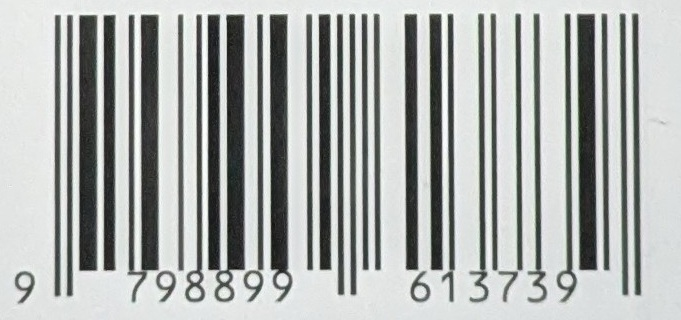
\includegraphics[width=0.3\linewidth,keepaspectratio]{sahajjeevan_isbn} \\ [0.5em]
ISBN-13 ‏ : ‎ XXX-XXXXXXX\\[1.5em]

कॉपीराइट-मुक्त © २०२५ डॉ. योगेश हरिभाऊ कुलकर्णी\\[0.5em]

{\textit{सर्व हक्क सार्वजनिक. या पुस्तकाचा कोणताही भाग प्रकाशकाच्या लेखी परवानगीशिवाय कोणत्याही स्वरूपात पुनर्मुद्रित किंवा पुनर्प्रकाशित करता येईल.}}\\[1.5em]

{\large Legal Notice:}\\
{\textit{This entire work is uncopyrighted. No rights reserved. Any part of this publication may be reproduced, distributed, or transmitted in any form or by any means, including photocopying, recording, or other electronic or mechanical methods, without the prior written permission of the publisher.}}
\end{flushleft}
\vfill\null
\clearpage

\begin{dedication}
मुक्त-स्रोत (`ओपन-सोर्स') चळवळीस  समर्पित  
\end{dedication}

\clearpage

\chapter*{पुस्तकाविषयी}
हे पुस्तक प्रामुख्याने दोन भागात आहे.  पहिल्या भागात लीओ बाबाउटा यांच्या 'द एफर्टलेस लाईफ' या पुस्तकाचा स्वैर अनुवाद आहे.  मूळ पुस्तक जगभरातील वाचकांच्या मदतीने इंग्रजीत सार्वजनिक पद्धतीने लिहिले गेले होते.  मूळ पुस्तकप्रमाणेच  हे भाषांतरसुद्धा  कोणत्याही हक्काधिकाराशिवाय (Uncopyrighted) उपलब्ध ठेवले आहे.  तर दुसऱ्या भागात लेखकासकट इतर सहयोग्यांनी पाठवलेले विचार असणार आहेत.  हा दुसरा भाग प्रवाही (live), सतत अद्ययावत असणार आहे .  
याचा प्रपंचाचा उद्देश मराठी वाचकांना ``सहज जीवन'' जगण्यासाठी मार्गदर्शन मिळावे हा आहे. 

\tableofcontents

\mainmatter
%%%%%%%%%%%%%%%%%%%%%%%%%%%%%%%%%%%%%%%%%%%%%%%
\chapter*{लीओ बाबाउटा यांच्या `द एफर्टलेस लाईफ' या पुस्तकाचा स्वैर अनुवाद}

%%%%%%%%%%%%%%%%%%%%%%%%%%%%%%%%%%%%%%%%%%%%%%%
\chapter*{लीओ बाबाउटा यांच्या `द एफर्टलेस लाईफ' या पुस्तकाचा स्वैर अनुवाद}

%%%%%%%%%%%%%%%%%%%%%%%%%%%%%%%%%%%%%%%%%%%%%%%
\chapter{परिचय}

जीवन कठीण आहे किंवा आपल्याला तसे वाटते तरी. 

पण खरी गोष्ट ही आहे की जीवन तेवढेच कठीण आहे जेवढे आपण ते समजतो-ठरवतो.

आपल्यापैकी बहुतेकजण दररोज अनेक कामांमध्ये आणि धावपळीत असतात, हे काम, त्यानंतर ते काम, काहीतरी  तडजोड अशा अनेक नाट्यमय प्रसंगांना सामोरे जात असतात. तुकोबारायांनी म्हटल्याप्रमाणे ‘रात्रंदिन आम्हा युद्धाचा प्रसंग’. पण नीट लक्ष दिले तर असे दिसेल की या संघर्षांपैकी बहुतेक गोष्टी काल्पनिक आणि उगाचच ओढून ताणून बोलावल्यासारख्या असतात.

आपण खरंतर अगदी साधे प्राणी आहोत. अन्न, वस्त्र, निवारा, आणि नातेसंबंध हे एवढेच आपल्याला आनंदी राहण्यासाठी पुरेसे आहेत. अन्न  नैसर्गिकपणे मिळते. वस्त्र म्हणजे कापड, तेही मिळते. निवारा म्हणजे छत, तेही आता बहुतेक सर्वांच्या डोक्यावर असते. नातेसंबंध म्हणजे अपेक्षांशिवाय एकमेकांच्या सहवासाचा आनंद घेणे. ते पण असतील तर बहारच. पण आपण मात्र या साध्या गरजांच्या पलीकडे, उगाचच काही काल्पनिक गरजा जोडल्या आहेत: करिअर, बॉस-सहकारी; नवीन यंत्रे (गॅजेट्स), सॉफ्टवेअर आणि सोशल मीडिया; गाड्या आणि छान कपडे, पर्स, लॅपटॉप बॅग, परदेशी सहल, आणि बरेच काही. 

मी असे म्हणत नाही की आपण अगदी आदिमानवाच्या काळात परत जावे, पण हे लक्षात ठेवणे महत्त्वाचे आहे की काय अगदी आवश्यक आहे आणि काय काल्पनिक आहे.

जेव्हा आपल्याला कळते की काहीतरी काल्पनिक आहे, तेव्हा आपण त्या गरजेला नाकारण्याचे ठरवू शकतो; जर ती चांगल्या-महत्वाच्या  उद्देशाची पूर्तता करत नसेल. जर ती जीवन अधिक कठीण बनवत असेल, तर ती सोडली-त्यागली जाऊ शकते! जीवन कठीण बनवणाऱ्या गोष्टी काढून टाकल्याने, आपल्याकडे जे उरते ते 'सहज जीवन'.

मला जेव्हा पट्टीचा पोहणारा बनायचे होते तेव्हा मी एक महत्त्वाचा धडा शिकलो.  मला वाटत होते की खूप लांब आणि वेगाने पोहणे यासाठी लागतं ते म्हणजे फक्त अधिक जोर लावणे आणि खूप वेळ तो प्रयत्न कष्टप्रद वाटलं तरी करत राहणे. म्हणून मी पाण्यात वेड्यासारखा हातपायमारत बसायचो, आणि मग थकून जायचो. पण जेव्हा मला हे उमगले की पाणी सुद्धा  तुम्हाला वर ढकलत असते आणि ते तरंगण्यास मदत करू शकते, तेव्हा मात्र त्यातून पोहणे खूप सोपे व्हायला लागले. मी मनात शांत आणि अतिप्रयत्नात शिथिल झालो, गोष्टींना जबरदस्तीने करण्याचा प्रयत्न थांबवला आणि कमी प्रयत्नाने चांगले पोहायला शिकलो, अगदी माशासाऱ्याखे. 
असं बघा, आयुष्य हा पण एक प्रवाह आहे. आयुष्य म्हणजे पाणी, आणि आपण मात्र त्याला हातपाय मारत राहतो, खूप धडपड करतो, जबरदस्तीने पुढे जायचा प्रयत्न करतो. शेवटी पदरात पडते  ती तगमग, आणि फुकाचा संघर्ष. खरं शहाणपण हेच आहे की आपल्याला असे विनाकारण कष्टदायक पोहोण्याची गरजच नाहीये, तर गरज आहे तरंगायला शिकायची. गोष्टींना जबरदस्तीने वळवायचं नाही, तर त्यांना सहजपणे घडू द्यायचं आहे. असं झालं की आपण जास्त आरामात पुढं जातो आणि आयुष्याचा गोडवा अधिक खुलतो. कदाचित ज्ञानोबारायांनीच म्हटले आहे की, ‘सहजी नीटू जाहला’. 
अशी कल्पना करा की तुम्ही सकाळी जागे होता आणि लगेच तुम्हाला आवडणारं काम करता. तुम्ही फक्त जगण्यासाठी नाही, तर जगण्याचा आनंद लुटण्यासाठी जगता. ज्या लोकांना तुम्ही मनापासून आवडता, त्यांच्यासोबत वेळ घालवता, आणि त्या प्रत्येक क्षणाला पुरेपूर जगता. त्या क्षणात तुम्ही इतके रमता की भविष्याची काळजी तुम्हाला बोचत नाही, आणि भूतकाळातील चुका तुमच्यावर ओझ्यासारख्या ओझं बनून राहात नाहीत. कुण्याकाळचे पाणीही डोळ्यात येत नाही (कवी: संदीप खरे). 

कल्पना करा, तुमच्याकडे काही मोजके जवळचे मित्र आणि जिवलग कुटुंबीय आहेत. तुम्ही त्यांच्यासोबत मोकळेपणाने, भरपूर वेळ घालवता. त्यांच्याकडून तुम्हाला कसल्याही अपेक्षा नसतात. म्हणूनच ते तुम्हाला कधी निराश करत नाहीत. उलट, ते जे काही करतात ते तुम्हाला अगदी योग्यच वाटतं. तुम्ही त्यांना त्यांच्या मूळ स्वरूपासाठी प्रेम करता, त्यांचं व्यक्तिमत्त्व जसं आहे तसं मान्य करता. त्यामुळे तुमची नाती कधीच गुंतागुंतीची होत नाहीत.

अजून कल्पना करा, की तुम्हाला एकांताचा आनंद घेता येतो. एकटं राहूनही तुम्ही समाधानी असता, तुमच्या स्वतःच्या विचारांसोबत, निसर्गाच्या सहवासात, एखाद्या पुस्तकात हरवून, किंवा कदाचित काहीतरी नवीन निर्माण करताना. हे सर्व स्वप्नवत, कदाचित आभासी आणि अशक्यप्राय वाटतं  ना? 

हेच खरं साधं, सहज जीवन आहे. आता सहज म्हणजे अजिबात प्रयत्न न करणं असा त्याचा अर्थ नाही. उलट, प्रयत्न होतात पण ते भारासारखे वाटत नाहीत. ते हलके वाटतात, सहजतेने घडतात. आणि शेवटी, हीच सहजतेची जाणीव महत्त्वाची ठरते.

आणि सगळ्यात खास म्हणजे, असं जीवन फक्त कल्पनेत नाही, तर प्रत्यक्ष जगता येणं  पूर्णपणे शक्य आहे.

सहज जीवनाच्या मार्गात जर कोणी अडथळा आणत असेल, तर ते दुसरं कोणी नसून आपलं स्वतःचं मन असतं.


%%%%%%%%%%%%%%%%%%%%%%%%%%%%%%%%%%%%%%%%%%%%%%%
\chapter{सहज जीवनासाठी मार्गदर्शक तत्त्वे}

जीवनात सहजता शोधायची असेल तर त्याचे नियम, तत्वे  कठोर नसावीत, तर काळानुरूप लवचिक आणि प्रवाही-जिवंत असावीत. इथे सांगितलेली तत्त्वे-नियम काही दगडावरची रेघ नाही, तर त्या सौम्य सूचना आहेत. आणि विशेष लक्ष द्यायचं म्हणजे ही तत्त्वे जाणीवपूर्वक ‘नकारात्मक’ स्वरूपात मांडलेली आहेत. कारण इथे कोणीही आपल्याला “काय करावे” हे शिकवायला आलेलं नाही. त्याऐवजी हे मार्गदर्शन फक्त एवढंच सांगतं की “काय करू नये”. कारण बऱ्याच वेळा आपल्या जीवनात जी घाईगडबड, गुंतागुंत आणि थकवा निर्माण होत असतो, तो आपण केलेल्या अनावश्यक प्रयत्नांमुळे असतो. हे प्रयत्न टाळले तरच सहजतेचा मार्ग खुला होतो. आणि मग उरलेला भाग, म्हणजे काय करायचं, कोणत्या दिशेने चालायचं, हे पूर्णपणे तुमच्या हाती आहे.

आयुष्य हा एक जणू नकाशा आहे, त्या नकाशावर चालण्याचा मार्ग तुम्हालाच निवडायचा आहे. वळणाचा की सरळ बरा? (कवी: सौमित्र)

\textbf{मार्गदर्शक तत्त्वे:}
\begin{itemize}
\item इतरांना कोणतीही हानी पोहोचवू नका. कारण दुखावणे म्हणजे आपल्या स्वतःच्याच मनःशांतीवर घाव घालणे होय.
\item कोणतेही लक्ष्य (गोल्स) कठोर, अतिनिश्चित अथवा अपरिवर्तनीय ठेवू नका, तसेच कोणत्याही योजना (प्लॅन्स)  आखीवरेखीव बनवू  नका. आयुष्य नेहमीच बदलत्या वाऱ्यासारखं असतं, त्याच्याशी जुळवून घ्यावं लागतं, लवचिकतेने.
\item अपेक्षा ठेवू नका. कारण अपेक्षा ही निराशेची जननी असते.
\item खोट्या किंवा दिखाऊ गरजा निर्माण करू नका. जे खरेच आवश्यक आहे, ते आपल्यापर्यंत आपोआप येते.
\item ज्या गोष्टी तुम्हाला आवडत नाहीत, त्या जबरदस्तीने करू नका. तिरस्कारातून केलेले काम नेहमीच ओझं बनतं.
\item घाईगडबड करू नका. घाई म्हणजे चुका, आणि चुका म्हणजे पुन्हा दुरुस्त्या.
\item अनावश्यक कृती टाळा. कमी करणे म्हणजेच कधी कधी जास्त साध्य करणे असते.
\end{itemize}


\textbf{काही संभाव्य सकारात्मक मार्गदर्शक तत्त्वे:}
\begin{itemize}
\item दयाळूपणे वागा. दया म्हणजे दुसऱ्याच्या डोळ्यांतून-भूमिकेतून अजमावण्याची-पाहण्याची ताकद.
\item उत्साहाने जगा. आयुष्य हे एका रंगमंचावरील नाटकासारखं आहे, तुम्हालाच रस नसेल तर इतर-प्रेक्षक सुद्धा उठून जातात.
\item समाधान शोधा. कारण समाधान म्हणजे खऱ्या श्रीमंतीचं मोजमाप.
\item हळूहळू चला. सावकाश चालण्यातही एक प्रकारची खोल शांतता असते.
\item संयम ठेवा. थांबण्याची ताकद ही धावण्यापेक्षा जास्त असते.
\item वर्तमान क्षणात जगा. कारण भूतकाळ केवळ आठवण आणि भविष्य फक्त कल्पना आहे.
\item बेरीजेपेक्षा वजाबाकीला प्राधान्य द्या. अनावश्यक गोष्टी काढून टाकल्यावरच आयुष्याचं सौंदर्य दिसतं.
\end{itemize}

ही तत्त्वे म्हणजे जीवन साधं करण्याचा एक सौम्य प्रयत्न आहे. थोडं थांबा, विचार करा आणि मगच पुढचं पाऊल टाका, एवढं पुरेसं आहे सहजतेसाठी.

%%%%%%%%%%%%%%%%%%%%%%%%%%%%%%%%%%%%%%%%%%%%%%%%%%%%%%%
 \chapter{वू वेई आणि निष्क्रियता तत्व}
‘ताओ’वादामध्ये एक संकल्पना आहे, तिचं  नाव ‘वू वेई’. ही आपल्या नेहमीच्या पाश्चिमात्य-आधुनिक विचारपद्धतीला सरळ सोप्या भाषेत पटवून देणे अवघड जाते. साधारणपणे तिचा अर्थ “न-करणे” किंवा “निष्क्रियता” असा आहे. पण मला मात्र (हे एका वाक्यात सांगायचं झालं तर) केव्हा ‘काहीच न करणे’ योग्य ठरते आणि कधी ‘कृती करणे गरजेचे असते’ हे ओळखणे, असा अर्थ अभिप्रेत आहे असे वाटते.
आपल्या आधुनिकजीवनशैलीत मात्र याचा स्वीकार करणे बिलकुल सोपे नाही. कारण आपली संपूर्ण संस्कृतीच काहीतरी सतत “करत राहणे”, ‘बिझी असणे’, कार्यमग्न असणे, या तत्त्वाभोवती फिरत आलेली आहे. आपल्याला नेहमी काहीतरी कृती करत राहिलं पाहिजे असं वाटतं. एखादी कृती न केल्यास किंवा थांबल्यास मनात एक विचित्र अस्वस्थता, चिंतेची रुखरुख जाणवते. या सततच्या “काहीतरी करत राहण्याच्या” सवयीमुळे आपण आयुष्यात बऱ्याच अडचणी उभ्या करतो. आपण फक्त “न-करणे” या साध्या अवस्थेला घाबरतो, आणि त्या भीतीपोटी अनावश्यक श्रम स्वतःवर लादतो.
पण थोडा विचार करा, खरंच काहीच न करणे शक्य आहे का? अक्षरशः म्हणाल तर नाही. आपण काम करत नसू, तरी आपण बसलेले असतो, आडवे पडलो असतो किंवा उभे राहिलो असतो. म्हणजे काहीतरी घडतच असतं. पण साधारणतः “कृती” म्हटल्यावर आपल्याला जे सुचतं ते म्हणजे एखादं काम, जे कोणत्या तरी ध्येयाकडे (लक्ष्य , गोल्स) किंवा हेतूकडे (पर्पझ) नेणारं असतं. जर आपणच तो हेतू किंवा ध्येय बाजूला ठेवलं, तर ती कृती अनावश्यक ठरते. उलट ती केल्यामुळे आयुष्य अधिकच गुंतागुंतीचं होऊ शकतं.
म्हणूनच, जर आपण लक्ष्यं आणि उद्दिष्टं कमी केली, त्यांना सुलभ, सुकर आणि सोपं केलं, तर आयुष्यातील अनेक गोष्टींना आपोआपच करण्याची गरज उरत नाही.
हा विचार मनाशी पक्का करणे मात्र फार कठीण आहे. कारण आपल्याला नेहमी “उत्पादक” (प्रोडक्टीव्ह) राहायची सवय जडलेली असते. “निष्क्रिय” (इनॅक्टिव्ह) या शब्दालाच आपल्या समाजाने इतके नकारात्मक अर्थ-भाव चिटकवले आहेत की आपल्याला काहीच न करणे म्हणजे आळस, अपयश किंवा वेळ वाया घालवणे असेच वाटते. आळशीपणाला आपली संस्कृती नेहमी हिणवते. म्हणून मग आपण नकळत अनावश्यक ध्येयं ठरवतो, कामं करतो, केवळ हे दाखवण्यासाठी की आपण काहीतरी करतोय.
पण जरा कल्पना करा, जर आपण स्वतःची किंमत आपल्या यशापयशाने किंवा कामगिरीवरून मोजणं थांबवलं, तर? आपल्या फक्त “आहे’पणाला” (बीइंग) नेहमीच “करत राहण्यापेक्षा” (डुईंग) अधिक महत्त्व असणार नाही का?
चला, एक छोटा प्रयोग करून बघा. काहीच न करण्याचा प्रयत्न करा. अगदी फक्त पाच मिनिटांसाठी. त्या पाच मिनिटांत आपण कासावीस होतो , बेचैन होतो, मनात येतं की नवीन टॅब उघडावा, ईमेल तपासावा, एखादा लेख वाचावा, कुणाला फोन करावा, किंवा एखादं छोटं काम उरकावं. आणि हे सगळं फक्त पाच मिनिटांत! मग जरा विचार करा, जर पूर्ण दिवस काहीच केलं नाही, तर आपलं काय हाल होईल?
जर आपण खोट्या-काल्पनिक गरजा, कृत्रिम ध्येयं, नुसत्या अपेक्षा आणि बनावट उद्दिष्टं दूर केली, तर आपल्या रोजच्या कृतींपैकी अर्ध्याहून अधिक कृतींचं अस्तित्वच नष्ट होईल. मग आपल्यासमोर एक असं रिकामं स्थान उरेल, जे फक्त खरी गरज, नैसर्गिक प्रवृत्ती आणि खरी सुंदरता यांनी भरून काढता येईल.
अशा त्या “काहीच न करण्याच्या” रिकामेपणातच खरी समृद्धी दडलेली आहे.


%%%%%%%%%%%%%%%%%%%%%%%%%%%%%%%%%%%%%%%%%%%%%%%%%%%%%%%
\chapter{खऱ्या आणि साध्या गरजा}

तर मग खरंच आवश्यक काय आहे? हा प्रश्न विचारताना आपल्याला समजते की माणसाच्या खऱ्याखुऱ्या गरजा अगदी मोजक्या आहेत,  अन्न, कपडे, निवारा आणि नातेसंबंध. या चार गोष्टींपलीकडे उरलेलं बरंचसं केवळ आपल्या समाजाच्या कल्पनेतून, आणि थोडंफार आपल्या अहंकारातून उभं राहिलेलं आहे.

या मूलभूत गरजांपैकी एकही गरज प्रत्यक्षात फारशी क्लिष्ट नाही.

उदाहरणार्थ, अन्न घेऊया. कोणी म्हणेल की अन्न मिळवणे हे फारच गुंतागुंतीचे काम आहे. पण मसानोबू फुकुओकाचे “वन स्ट्रॉ रिव्होल्यूशन” वाचले की डोळे उघडतात. तो दाखवतो की फक्त एक एकर जमिनीवरही एका कुटुंबासाठी पुरेसं अन्न उगवता येतं, आणि त्यासाठी निसर्गात फारसा हस्तक्षेप करण्याची गरजही नाही. तण जसं वाढतं तसं वाढू द्या, कीटकनाशकांचा वापर करू नका, जमिनीची सतत नांगरट करू नका, आणि प्राणी, कीटक, सरडे शेतामध्ये मोकळेपणाने फिरू द्या. हे चित्र बघितलं तर लक्षात येतं,  अन्न उगवणं खरं तर अवघड नाही.

याचा अर्थ असा अजिबात नाही की आपण सगळे उद्या आपापली नोकरी सोडून जमिनीवर शेती करायला लागणार आहोत. पण इतकं लक्षात ठेवायला हरकत नाही की आपल्या अन्नाची खरी गरज समाजाने क्लिष्ट करून टाकली आहे. आज अन्न हे पोषण देणाऱ्या साध्या गोष्टीऐवजी  सामाजिक पत -स्थान-उंची-दर्जा (“स्टेटस सिम्बॉल”) बनलं आहे. अन्न महागडं, ब्रँडेड किंवा दिखाऊ असलं तरच त्याला किंमत आहे असं मानलं जातं. पण खरं म्हणजे साधं अन्न पुरेसं असतं, आणि जीवन साधं करण्याची ताकद इथूनच सुरू होते, जे नको त्यांची वजाबाकी करून.

निवाऱ्याचंही अगदी तसंच झालं आहे. घर ही बहुतांश लोकांसाठी आयुष्यातील सर्वात मोठी गुंतवणूक असते. एक सुंदर, मोठं, सजवलेलं घर सुद्धा आज “स्टेटस सिम्बॉल” मानलं जातं. पण मूळात निवारा म्हणजे एवढंच असतं  की,  हवामान, पाऊस, उन्हापासून आपलं रक्षण करणारी जागा, छत. ते एखाद्या माणसासाठी छोटं शेड असू शकतं किंवा काही कुटुंबांसाठी जरा मोठं आश्रयस्थान. त्याला भव्यतेची गरज नाही. हवं तर ते अगदी साधं असू शकतं.

कपड्यांबद्दलही हेच खरे. एक काळ होता जेव्हा कपडे ही केवळ अंग झाकण्याची गरज होती. पण आज कपडे हे इतके गुंतागुंतीच्या पद्धतीने, पुन्हा, “स्टेटस सिम्बॉल” झाले आहेत की त्यांचा खऱ्या गरजेशी संबंध उरलेलाच नाही. खरेतर आपल्याला फक्त शरीर झाकायला काहीतरी हवे. गांधीजींनी दाखवून दिलं होतं,  हाताने कातलेलं साधं कापड पुरेसं आहे. आपण आता सगळे फक्त पंचा परिधान करायला लागणार नाही, हे खरं. पण किमान हे लक्षात ठेवायला हवं की आपल्या कपड्यांपैकी किती गरजेपुरतं आहे आणि किती फक्त कल्पनेतून निर्माण झालंय.

नातेसंबंध या चारही गरजांमध्ये सर्वात गुंतागुंतीचे आहेत. कारण माणसं हे गुंतागुंतीचे “प्राणी” आहेत. आपल्याला ‘आपलेपण’ हवं असतं, इतरांच्या नजरेत चांगले दिसावं असं वाटत असतं, आपल्याला आकर्षक भासायचं असतं. आणि म्हणूनच नातेसंबंध ही भावनांचा, अपेक्षांचा आणि परस्परसंवादांचा एक असा गुंतागुंतीचा तिढा बनतो की तो सहजासहजी सुटतच नाही.

पण हे सर्व खरंच इतकं कठीण असायलाच हवं असं काही बिलकुल नाही. जेव्हा मी एका मित्राला भेटतो. त्या क्षणी उरलेलं जग बाजूला ठेवून मी फक्त त्या भेटीत उपस्थित राहतो. आम्ही बोलतो, विनोद करतो, आणि एकमेकांकडून काही अपेक्षा बाळगत नाही. मग आम्ही निरोप घेतो तेव्हा मनात कुठलीही कटुता किंवा पुन्हा कधी भेटणार याची चिंता राहत नाही. इतकं साधंही नातं असू शकतं.

नक्कीच, माझं लग्न किंवा माझ्या मुलांबरोबरचे नातेसंबंध इतके सरळ नाहीत. पण मी शिकतोय की अपेक्षा कमी केल्या, मागण्या घटवल्या तर जे उरतं ते म्हणजे प्रत्येक नात्याचं खरं सौंदर्य,  प्रत्येक व्यक्तीला जशी आहे तशी स्वीकृती. अजून मी पूर्णपणे इथे पोचलो नाहीये, पण शिकतोय. अनावश्यक अपेक्षांची वजाबाकी केली की जे उरतं ते म्हणजे नात्याचं सार.

समाजाशी आपलं नातंही असंच असतं. नोकरीच्या माध्यमातून आपलं योगदान ठरवलं जातं. पण ती नोकरी आपल्या आयुष्याचा मोठा भाग खाते, आणि ताण, निराशा निर्माण करते. का? कारण आपण बनावट गरजा पूर्ण करण्यासाठी अधिकाधिक तास काम करतो. जर आपण आपल्याच गरजा कमी केल्या आणि कमी गोष्टींमध्ये समाधान मानायला शिकलो, तर खरं म्हणजे फार थोडं काम केलं तरी जगता येतं.

मग उरतो भरपूर वेळ, समाजासाठी साध्या पण महत्त्वाच्या मार्गाने काहीतरी देण्यासाठी. आपण धर्मादाय संस्थांमध्ये स्वयंसेवक म्हणून काम करू शकतो, आपल्या शेजाऱ्यांना मदत करू शकतो, काहीतरी सुंदर निर्माण करू शकतो. आपल्याला हवं तर आपण चांगलं काम करू शकतो आणि ते केल्यावर लगेच सोडून देऊ शकतो,  बक्षीस, कौतुक किंवा मोबदल्याची अपेक्षा न ठेवता. किंवा फक्त उपलब्ध राहू शकतो, म्हणजे इतरांना गरज असेल तेव्हा आपण सतत आपल्या ध्येयांच्या मागे धावत नसू.

शेवटी गोष्ट अगदी सरळ आहे. आपल्या खऱ्याखुऱ्या गरजा अगदी साध्याच आहेत. बाकीचं सगळं आपण स्वतःहून ओढवून घेतलेलं ओझं आहे.

%%%%%%%%%%%%%%%%%%%%%%%%%%%%%%%%%%%%%%%%%%%%%%%%%%%%%%%
 \chapter{आपल्या गरजा कमी करा}
मी आधीच म्हटल्याप्रमाणे, आपल्या खऱ्याखुऱ्या गरजा फारशा नसतात, त्या अगदी साध्या आणि मर्यादित असतात. पण आधुनिक समाजात आपण स्वतःभोवती नवनवीन गरजा जोडत गेलो आहोत. आलिशान घर हवे, भारी कपडे हवेत, महागडी गाडी हवी, गॅजेट्स-कॉम्प्युटर,उंची शौक, नेहमी बाहेर खाणे, परदेशी सहली, करमणूक (एंटरटेनमेंट), परदेशी शिक्षण आणि अजून बऱ्याच गोष्टींसाठी आपल्याला नोकरीची गरज भासते. म्हणजे, मूलभूत गरजा पूर्ण करण्यापेक्षा अधिकाधिक खर्च करण्यासाठीच आपण आयुष्य झिजवत असतो.
पण जर आपण आपल्या गरजा हळूहळू कमी करायला सुरुवात केली, आणि "कमी मिळालं तरी मी आनंदी राहीन" अशी सवय लावली, तर मग जीवन सोपं होऊ लागतं. गरजा कमी म्हणजे खर्च कमी. खर्च कमी म्हणजे कष्ट आणि धडपडही कमी आणि कमी धडपडीमुळे आयुष्यात थोडा श्वास घ्यायला, हसतखेळत राहायला जास्त वेळ मिळतो.
जेव्हा आपल्याकडे कमी गरजा असतात, तेव्हा यशस्वी व्हायचे दडपणही कमी असते. सतत पुढची उंची गाठण्याची हाव लागत नाही. त्यामुळे मन जास्त शांत राहतं, काळजी कमी होते, कारण काळजी करण्यासारखं फारसं उरतच नाही.
गरजा कमी करण्याची ही प्रक्रिया रातोरात साध्य होत नाही. ही सजगपणे (माइंडफुल) आणि हळूहळू करायची गोष्ट आहे. पहिल्यांदा आपले खर्च नीट पहा. आठवड्यात आपण कोणकोणत्या गोष्टींवर किती-किती पैसे खर्च करतो, कोणत्या सवयी जोपासतो, हे स्वतःला विचारा. आणि मग त्यातील कोणत्या गोष्टी खरंच आवश्यक आहेत याचा विचार करा.
थोडं थोडं करून अनावश्यक गोष्टी बाजूला काढायला लागा. उदाहरणार्थ, रोजच्या रोज ‘सी-सी-डी‘ किंवा ‘स्टारबक्स’ मधली महागडी कॉफी खरंच हवी का? की तुम्ही घरी स्वतः छान कॉफी बनवू शकता, किंवा त्याऐवजी साधं पाणी पिऊनही आनंदी राहू शकता? महागड्या फराळाची (स्नॅक्स) खरंच गरज आहे का? की फळं, सुकामेवा यातून अधिक आरोग्यदायी आनंद घेऊ शकता? महागड्या करमणुकीमध्ये (एंटरटेनमेंट) भाग घ्यायलाच पाहिजे का? की आपल्या मुलांसोबत खेळणं, उद्यानात मित्रांसोबत वेळ घालवणं यातूनही तितकाच खरा आनंद मिळू शकतो. खरंच त्या महागड्या जिमचं सदस्यत्व हवं का? की मग जोडीदारासोबत रोज फेरफटका मारणं, बाहेरच पुश-अप्स करणं, सूर्यनमस्कार घालणं पुरेसं ठरू शकतं?
हळूहळू मोठ्या खर्चांकडे पाहायला लागा. खरंच दोन गाड्यांची आवश्यकता आहे का? मोठ्या गाडी (एस-यू-व्ही) ऐवजी एखादी लहान, कमी किमतीची वापरलेली गाडी पुरेशी ठरू शकत नाही का? गाडी सोडून सार्वजनिक वाहतूक म्हणजे बस-रिक्षा (पब्लिक ट्रान्सपोर्ट) किंवा जवळच्या अंतरांसाठी सायकलने काम भागवता येईल का? इतक्या मोठ्या घराची गरज आहे का? की मग कमी किमतीचं, उष्णतेसाठी वा थंडीसाठी कमी खर्चाचं घर पुरेसं होऊ शकतं? शिक्षणाचा खर्च इतका महाग असायलाच हवा का? की मग स्वशिक्षणाने, मोफत उपलब्ध साधनांचा वापर करून आपण ज्ञान मिळवू शकतो?
मी इथे असं सांगत नाही की या सगळ्या गोष्टी तात्काळ सोडून द्या. माझा हेतू एवढाच आहे की आपण स्वतःला प्रश्न विचारावा, खर्च कुठे होतोय हे ओळखावं, आणि हळूहळू अनावश्यक गोष्टी कापत नेऊन फक्त प्रमुख आणि अत्यावश्यक गोष्टींवर लक्ष केंद्रित करावं.
खरंतर, आयुष्यातला खरा आनंद देणाऱ्या गोष्टींसाठी फार खर्च करावा लागत नाही. माझ्यासाठी गरजेच्या आणि मला खऱ्या अर्थाने सुख देणाऱ्या गोष्टी या अगदी साध्या आहेत :
\begin{itemize}
 \item एक चांगलं पुस्तक, जे सहजपणे ग्रंथालयात मिळतं.
 \item लिहिण्यासाठी वही किंवा साधा कॉम्पुटर-लॅपटॉप
 \item रोजचं बाहेर पायी चालणं.
 \item माझ्या पत्नीसोबतचा साधा, पण मनाला उल्हसित करणारा चहा.
 \item माझ्या मुलांसोबत खेळण्यातला निरागस आनंद.
 \item एखाद्या मित्रासोबत धावायला जाणं.
 \end{itemize}
मूलभूत गरजा, म्हणजे अन्न, कपडे, निवारा यांच्यापलीकडे, खरंतर आनंदी राहायला मला एवढंच लागतं. आणि लक्षात घ्या, या सर्वांची आर्थिक किंमत फारच कमी आहे.
गरजा कमी करा. साधेपणात समाधान शोधा. मग बघा, जीवनासाठी लागणारा प्रयत्न, संघर्ष, धडपड कित्येक पटींनी कमी होतो. आयुष्य हलकंफुलकं आणि सुखद होतं.

%%%%%%%%%%%%%%%%%%%%%%%%%%%%%%%%%%%%%%%%%%%%%%%%%%%%%%%
\chapter{हानी करू नका आणि दयाळूपणे जगा}
हा माझ्या आयुष्याचा मूलभूत नियम आहे. तो अगदी साधा दिसतो, पण त्याने मला आतापर्यंत खूप आधार दिला आहे. खरं सांगायचं तर, या नियमामुळे माझं जीवन जरा हलकंफुलकं झालं, भार कमी झाला. त्याचे परिणाम अगदी रोजच्या जगण्यात दिसतात. उदाहरणार्थ, 
\begin{itemize}
 \item नातेसंबंध अधिक सोपे, सुसंवादी आणि समाधान देणारे झाले.
 \item लोक आपोआपच माझ्याशी थोडं अधिक प्रेमळ, सौम्य आणि दयाळूपणे वागतात.
 \item दयाळू व्यक्ती म्हणून लोकांच्या मनात प्रतिमा निर्माण झाली की, समाजात अनेक दारे आपोआप उघडू लागतात.
 \item माझ्या मनात रोजच्या आयुष्यातील समाधानाची आणि आनंदाची पातळी वाढली.
 \item माझ्या आजूबाजूच्या लोकांच्या चेहऱ्यावरही थोडं अधिक हसू उमटलं, कारण आनंद संसर्गजन्य असतो.
 \end{itemize}
सहज जीवन (एफर्टलेस लाईफ)  या तत्त्वज्ञानाचा पहिला आणि सर्वात महत्त्वाचा नियम म्हणजे,  ‘हानी करू नका’. हा नियम पहिल्यांदा मांडला जातो, कारण तो उरलेल्या सर्व नियमांवर छाप टाकतो. धरून चालू की, “घाई करू नका” हा नियम पाळताना कुणाला हानी होणार असेल, तर अशावेळी तुम्ही “घाई करू नका” या नियमाला मागे सारून “हानी करू नका” या नियमाला अग्रक्रम द्यायला हवा.
कारण, जेव्हा आपण कुणाला हानी पोहोचवतो, तेव्हा समस्या ही फक्त त्या क्षणापुरती मर्यादित राहत नाही. ती पाण्यावर दगड टाकल्यावर उठणाऱ्या वलयांसारखी सर्वत्र पसरते. त्यामुळे तुमचं स्वतःचं जीवन गुंतागुंतीचं होतं, आणि ज्यांना तुम्ही त्रास दिला आहे, त्यांचं जीवनसुद्धा कठीण होतं. त्यानंतर तुम्हाला चुका दुरुस्त करण्याची, भरपाई करण्याची आणि क्षमा मागण्याची वेळ येते. हा प्रवास फार लांबणारा आणि नीरस असतो, आणि खरं तर तो आधीच टाळता येण्यासारखा होता.
दैनंदिन जीवनात हे नियम कसे लागू होतात? काही उदाहरणे अशी, 
\begin{itemize}
 \item इतरांना जाणीवपूर्वक मारू नका किंवा त्यांच्यावर हिंसा करू नका.
 \item प्रदूषण करून इतरांच्या आरोग्यावर परिणाम करू नका.
 \item मद्यपान करून गाडी चालवू नका, किंवा बेफिकीरपणे असे काहीही करू नका ज्यामुळे इतरांना इजा होऊ शकेल.
 \item प्राणी किंवा प्राणिजन्य पदार्थ खाऊ नका, कारण त्यातूनही हानीच होते.
 \item इतरांना अन्यायकारक व दडपशाहीच्या परिस्थितीत कामाला लावू नका, किंवा अशा मजुरांच्या, विशेषतः बालमजुरांच्या, श्रमातून निर्माण झालेल्या वस्तूंचा वापर टाळा.
 \item इतरांना संकटात टाकणारी चुकीची किंवा दिशाभूल करणारी माहिती पसरवू नका.
 \item चोरी करू नका, किंवा इतरांचे हक्काचे सामान बळकावू नका.
 \item कुणाच्या जगण्याला आधार देणारी साधने, संसाधने रोखून धरू नका.
 \item तुमच्या डोळ्यासमोर इतरांना त्रास दिला जात असेल तर शांत राहून किंवा निष्क्रिय राहून पाठींबा देऊ नका.
 \item जसं वागणं तुम्हाला स्वतःला नकोसं वाटेल, तसं इतरांशी करू नका.
 \item तुमचे वैयक्तिक विचार, धार्मिक श्रद्धा किंवा मतं इतरांवर जबरदस्ती लादू नका.
 \item खोटं बोलून विश्वास तोडू नका.
 \item खरी गरज नसताना वस्तू विकत घेऊ नका,  कारण प्रत्येक अनावश्यक खरेदीतून पर्यावरणाला हानी होते.
 \end{itemize}
अनेक वेळा “हानी करू नका” हा नियम सोपा नसतो. तुम्हाला बसून विचार करावा लागतो की कोणती कृती (किंवा कृती न करणे) कमी हानीकारक आहे. योग्य निर्णय काढणं नेहमीच सहज होत नाही, पण प्रयत्न मात्र करावा लागतो.
या तत्त्वाचा उजवा, सकारात्मक पैलू म्हणजे,  ‘दयाळूपणे जगा’ (बी कंपॅशनेट). हा नियम प्रत्यक्षात आपल्या विचार करण्याच्या सवयींचं रूपांतर करायला लावतो. उदाहरणार्थ, इतरांशी न्याय करणे. टीका करणे अथवा दोष काढणे याऐवजी, दयाळूपणा म्हणजे इतरांना समजून घेण्याचा प्रामाणिक प्रयत्न करणे. त्यांच्या मनात शिरून पाहणं, त्यांच्या वेदनांशी सहानुभूती दाखवणं आणि त्यांच्या त्रासात मनापासून दिलासा देणं.
दयाळूपणे जगणं हे एवढे मोठे आणि सखोल तत्व-चिंतन आहे की त्यावर स्वतंत्र पुस्तक लिहिता येईल. दलाई लामांचे “आनंदाची कला” (द आर्ट ऑफ हॅपिनेस) हे पुस्तक मी इथे सुचवेन. थोडक्यात सांगायचं तर, दयाळूपणा म्हणजे समजूतदारपणा, सहानुभूती, इतरांचे दुःख हलकं करण्याची इच्छा आणि त्यांच्या जीवनात आनंद वाढवण्याचा सातत्यपूर्ण प्रयत्न. अंगीकारून तर बघा. 











%%%%%%%%%%%%%%%%%%%%%%%%%%%%%%%%%%%%%%%%%%%%%%%%%%%%%%%
\chapter{कोणतेही लक्ष्य किंवा ठरलेली योजना ठेवू नका}
ठराविक, हातात मावतील अशी साध्य करता येणारी ध्येये असावीत, ही कल्पना आपल्या संस्कृतीत जणू काही जन्मतःच रोवलेली आहे. अगदी लहानपणापासून आपण ऐकत आलो आहोत की “ध्येयाशिवाय जीवन म्हणजे दिशाहीन प्रवास.” मी स्वतः अनेक वर्षे ध्येयांच्या मागे धावत राहिलो. खरं सांगायचं तर माझ्या आधीच्या लिखाणाचा मोठा भाग हा ध्येये कशी ठरवायची, त्यांची आखणी कशी करायची आणि ती पूर्ण करण्यासाठी काय करायला हवं याभोवतीच फिरत होता.
परंतु आजकाल माझं जीवन पूर्णपणे वेगळ्या वाटेने चालतंय. आता मी प्रामुख्याने ध्येयांशिवाय जगतो. आणि गंमत म्हणजे, यात एक विलक्षण स्वातंत्र्य आहे. लोकांना शिकवलं जातं की ध्येये न ठेवल्यास आयुष्य हातातून निसटून जाईल. पण माझा अनुभव अगदी उलट आहे. ध्येये नसली तरी तुम्ही काही साध्य करणं थांबवत नाही; उलट, तुम्ही स्वतःला कृत्रिम मर्यादांमध्ये अडकवणं थांबवता.
लोकप्रिय समजुतीत असं मानलं जातं की,  “जर तुम्हाला कुठे जायचं आहे हे ठाऊक नसेल, तर तुम्ही कुठेच पोहोचणार नाही.” (You’ll never get anywhere unless you know where you’re going). पहिल्यांदा ऐकल्यावर हे अगदी तर्कसंगत वाटतं. पण जर शांत बसून विचार केला, तर ही गोष्ट किती उथळ आहे हे लक्षात येतं. एक साधा प्रयोग करून बघा. घराबाहेर पडा आणि एखाद्या निव्वळ सहज सुचलेल्या दिशेने चालत राहा. चालताना मनात आलं की दिशा बदला. वीस मिनिटं, किवा एखादा तास असे भटकून बघा. तुम्ही नक्कीच कुठेतरी पोहोचाल. फरक फक्त इतकाच की तुम्हाला आधीपासून ठाऊक नसेल की तुम्ही नेमकं कुठे उतरणार आहात.
यातूनच खरा धडा मिळतो. तुमचं मन खुलं ठेवलं, तर तुम्ही कधीच न कल्पिलेल्या ठिकाणी जाऊन पोहोचता. ध्येयांशिवाय जगलात, तर नवीन प्रदेशांची सफर करता. अनपेक्षित शिकवणी मिळते. नवनवीन अनुभवांच्या धबधब्यात तुम्ही स्वतःला झोकून देता. जिथे जायची कधी कल्पना केली नसेल, तिथे स्वतःला गवसलेलं बघता. हे या विचारसरणीचं खरं सौंदर्य आहे. पण खरं सांगायचं तर, हा बदल स्वीकारणं अवघड असतं. कारण ध्येय ठरवण्याची सवय ही आपल्या अंगात पिढ्यान्पिढ्या रुजलेली आहे.
आज मी बहुतेक वेळा ध्येयांविना जगतो. कधीमधी नकळत एखादं ध्येय डोक्यात येतं. पण मी ते धरून बसत नाही; मी त्याला जाऊ देतो. खरं म्हणजे, ध्येयांशिवाय जगणं हे स्वतःमध्ये माझं कोणतं तरी ठरवलेलं ध्येय नव्हतंच. ही तर एक जीवनशैली आहे जी मला चालता चालता सापडली आहे. यात एक गोड दिलासा आहे, एक मुक्तता आहे, आणि सगळ्यात महत्त्वाचं म्हणजे,  यात मला माझ्या आवडीचं काम मनसोक्त करता येतं.

\section*{तीन महत्त्वाच्या नोंदी}

अनेकांना माझ्या \textbf{“लक्ष्य नाही” (\`\`No Goals'')} या प्रयोगाबद्दल आक्षेप असतो. लोकांना हा विचार पटत नाही किंवा फारच अतिरेकी वाटतो. म्हणूनच, या प्रयोगामागचा विचार स्पष्ट होण्यासाठी, आधी तीन महत्त्वाच्या नोंदी मांडतो.

पहिली नोंद ही \textbf{“लक्ष्य”} या शब्दाच्या व्याख्येबद्दल आहे.
मी लक्ष्य म्हणजे \textbf{“काहीही करायची इच्छा” (`anything you want to do'')} असे मानत नाही. इच्छा असणे हे माणसाच्या जगण्याचा नैसर्गिक भाग आहे. इथे माझा मुद्दा हा आहे की आपण आधीच डोक्यात ठरवलेले परिणाम, म्हणजेच \textbf{“पूर्वनिर्धारित outcome” (`predefined outcome'')} किंवा ठराविक गंतव्यस्थान, यांना सोडून द्यावे. उदाहरण घ्या. तुम्ही चालायला लागलात, पण कुठे जायचे हेच माहीत नाही. तरीही तुम्ही म्हणता, \textbf{“मी चालण्याचे लक्ष्य ठेवले आहे!”} (`I have a goal of walking!''). पण खरं पाहता, त्या चालण्यात ठराविक ठिकाण नाही. उलट, जर तुम्ही दुकानात जाण्यासाठी चालायला निघालात, तर तो प्रवास स्पष्ट लक्ष्य असलेला आहे. त्यामुळे जेव्हा लोक म्हणतात, \textbf{“तुम्ही काहीतरी करत आहात, म्हणजे तुमची लक्ष्ये आहेतच!”} (`You’re doing something, so therefore you have goals!''), तेव्हा माझे उत्तर असते, \textbf{“होय, मी करत आहे, पण मला ते कुठे नेईल याची मला कल्पना नाही, आणि प्रामाणिकपणे सांगायचे तर मला त्याची चिंता नाहीसुद्धा.”} (`Yes, but I don’t know or care where it takes me.'')  
आणि हे सांगून ठेवतो,  हे \textbf{“गॉचा सिंड्रोम” (`Gotcha Syndrome'')} नावाच्या वृत्तीचे लक्षण आहे. यात लोक शिफारसी स्वतः वापरून बघण्याऐवजी माझ्या म्हणण्यातल्या लहानमोठ्या विरोधाभासांवर बोट ठेवण्याचा खेळ खेळतात.

दुसरी नोंद अशी की, \textbf{तुम्हाला हा प्रयोग करून पाहण्याची अजिबात गरज नाही.}
जर लक्ष्यांशिवाय जगणे तुम्हाला अगदी हास्यास्पद, अतिरेकी किंवा “जगण्याला अर्थ नाही” असे काहीसे वाटत असेल, तर निश्चिंत रहा,  हा प्रयोग तुमच्यासाठी नाही. याबाबत तुम्ही माझ्याशी असहमत असलात तरी त्यात मला काही फरक पडत नाही. हा प्रयोग माझ्यासाठी काम करतो, पण कदाचित तुमच्यासाठी अजिबात करणार नाही. आणि तेही अगदी ठीक आहे. या पुस्तकात इतर बर्‍याच गोष्टी आहेत ज्या तुमच्यासाठी उपयुक्त ठरू शकतात. आणि कोण जाणे, कदाचित भविष्यात एखाद्या दिवशी तुम्ही या विचाराकडे परत याल, आणि त्याकडे वेगळ्या नजरेने पाहाल.

तिसरी आणि शेवटची नोंद,  \textbf{मला सुरुवातीला लक्ष्यांची खरंच गरज होती का?}
अनेक लोक म्हणतात, “तुला आता लक्ष्यांची गरज नाही, कारण तू आधीच बरंच काही साध्य करून बसला आहेस. जेव्हा माणूस एवढा पुढे गेला, तेव्हाच तो ‘लक्ष्य नाही’ म्हणू शकतो.” हे म्हणणे ऐकायला वाजवी वाटते. तुम्हाला हवे असल्यास तुम्ही हा मुद्दा मान्य करून बसू शकता. पण एक पर्याय असा आहे की,  एकदा स्वतःच प्रयत्न करा. एकदा जगून बघा, काम करून बघा, अगदी लक्ष्ये न ठेवता. आणि मग बघा काय होते ते.
मी स्वतः सुरुवातीला खरंच लक्ष्यांची गरज होती का? हे आता मागे वळून कसे तपासणार? भूतकाळाकडे जाऊन प्रयोग करून बघणे शक्य नाहीच. पण माझा अंदाज असा आहे की जर मी अगदी सुरुवातीपासून हा “लक्ष्यांशिवाय” प्रयोग केला असता, तर मी आज जिथे आहे तिथे पोहोचणार नाही कदाचित. पण याचा अर्थ असा नाही की मी वाईट ठिकाणी असतो. उलट, मी कुठेतरी दुसर्‍या सुंदर, समाधानकारक ठिकाणी असतो. जगण्याच्या प्रवासात शेवटचं ठिकाण मोजण्यापेक्षा चालण्याचा अनुभवच जास्त महत्त्वाचा असतो.


\section*{लक्ष्यांची समस्या}
भूतकाळात, मी वर्षाची सुरुवात होताच एखादे मोठे लक्ष्य किंवा किमान दोन-तीन तरी ठरवायचो. मग त्या वार्षिक ध्येयाला गाठण्यासाठी महिन्यागणिक लहान उप-लक्ष्ये आखली जात. पुढे त्याचे अजून विघटन करून आठवड्यागणिक, आणि शेवटी दिवसागणिक कृतीच्या पायऱ्या तयार होत. त्या कृतींवर माझा दिवस केंद्रित करण्याचा मी जीव तोडून प्रयत्न करायचो.
पण खरे सांगायचे झाले तर हे गणित इतक्या सरळसोटपणे कधीच जुळून येत नाही. हे सगळ्यांनाच ठाऊक आहे. आयुष्यात अचानक काही कामे घुसतात, वेळेचा ताण येतो, कधी टाळाटाळ तर कधी आळस हावी होतो. आणि मग होते काय, मासिक आणि साप्ताहिक लक्ष्ये मागे सरकतात, थांबून राहतात किंवा पूर्णपणे रुळावरून घसरतात. त्यातून मनात निराशा घर करून बसते कारण आपल्यात शिस्त नाही, आत्मसंयम नाही, असे वाटू लागते. मग आपण पुन्हा एकदा बसतो, आपली जुनी ध्येये उघडतो, त्यांचा आढावा घेतो, काहीतरी सुधारणा करून नवी ध्येये ठरवतो. उप-लक्ष्यांची आणि क्रियापद्धतीची ताजी यादी तयार होते.
कधीमधी एखादे ध्येय खरंच गाठले जाते आणि त्या क्षणी आपण स्वतःला हिरो समजतो, अप्रतिम वाटते. पण वस्तुस्थिती अशी की बहुतांश वेळा ध्येये गाठली जात नाहीत आणि त्याचे ओझे आपण स्वतःच्या डोक्यावर घेतो. चूक आपलीच आहे, आपणच निकामी ठरलो, अशी अपराधी भावना वाढत जाते.
खरे गुपित येथे आहे: समस्या तुमच्यात नाही, समस्या या संपूर्ण यंत्रणेच्या (system) रचनेत आहे. \textbf{लक्ष्य-केंद्रित व्यवस्था ही प्रत्यक्षात अपयशासाठीच घडवलेली आहे.}
कारण जरी तुम्ही पुस्तकात लिहिल्याप्रमाणे, नियमाप्रमाणे, अगदी बिनचूक वागलात तरीही ही प्रणाली आदर्श नाही. ध्येये तुमच्या क्षमतेभोवती भिंत उभी करतात, संधी कमी करतात. कधी तुम्हाला एखादी गोष्ट मनापासून करायची इच्छा नसते, पण फक्त ध्येय ठरवल्यामुळे तुम्हाला स्वतःला ओढूनताणून ती करावीच लागते. तुमचा मार्ग आधीच आखलेला असल्याने नवीन संधींचा शोध घेण्याची जागा उरत नाही. योजना ठरवलेली असल्याने तिचे पालन करावेच लागते, जरी त्या क्षणी तुमच्या मनाचा ओढा एखाद्या वेगळ्याच विषयाकडे असेल तरी.
काही ध्येय-प्रणाली लवचिक असतात, यात शंका नाही. पण खरी गोष्ट अशी आहे की ध्येयरहित आयुष्याइतके मोकळे, लवचिक आणि विस्तारासाठी उघडे काहीच नाही.
 \section*{लक्ष्यांशिवाय जगणे}
तर, \textbf{लक्ष्यांशिवायचे जीवन} नक्की कसे दिसते? व्यवहारात ते लक्ष्यांवर आधारलेल्यापेक्षा पूर्णपणे वेगळे असते. साधारणपणे आपल्याला लहानपणापासूनच “वार्षिक लक्ष्य”, “महिन्याचे उद्दिष्ट”, “आठवड्याचे प्लॅन” आणि अगदी “दिवसाचे टू-डू” अशी यादी ठेवायला शिकवले जाते. पण इथे चित्र उलट आहे, तुम्ही वर्षासाठी ध्येय ठरत नाही, महिन्यासाठी मापदंड आखत नाही, आठवड्याचा अजेंडा बांधत नाही आणि रोजची यादी तयार करत नाही.
तुम्ही \textbf{ट्रॅकिंग} \hspace{0.2cm}(Tracking) या संकल्पनेचा मागोवा घेत बसत नाही, प्रत्येक कृतीला टप्प्याटप्प्याने मोजत नाही. अगदी \textbf{टू-डू लिस्ट} \hspace{0.2cm}(To-do list) हवीच असे बंधनसुद्धा नाही. हो, आवडेल तर थोड्या आठवणी वहीत लिहून ठेवल्या तरी काही बिघडत नाही. पण त्या न लिहिल्या, तरी आयुष्य विस्कळीत होत नाही.
मग प्रश्न येतो, असं असताना दिवस कसा गेला म्हणायचा? तुम्ही दिवसभर सोफ्यावर लोळत बसता का? अजिबात नाही. तुम्ही जे काही खऱ्या अर्थाने आतून आवडते, ज्याबद्दल आतून ज्वाला पेटते ते शोधता आणि मग ते करता. “ध्येय नाही” म्हणजे “काहीही काम नाही” असं नव्हे. उलट, यातूनच नव्या निर्मितीला वाव मिळतो. तुम्ही काहीतरी घडवू शकता, नवे तयार करू शकता, आपल्या आवडीच्या दिशेने वाहू शकता.
हे प्रत्यक्ष अनुभवात अधिकच अद्भुत ठरते. सकाळी जागे झाल्यावर नेमके ध्येयाच्या चौकटीत न अडकता तुम्ही थेट आपल्या आवडीकडे वळता. माझ्यासाठी ते बहुधा \textbf{लेखन} असते. पण हे फक्त लेखनापुरते मर्यादित नाही. ते इतरांना मदत करणे असू शकते, अद्वितीय लोकांशी संबंध जोडणे असू शकते, पत्नीबरोबर वेळ घालवणे असू शकते, किंवा मुलांबरोबर खेळण्यात रमणे असू शकते. संधी आणि शक्यता या अमर्याद आहेत, कारण मी मोकळा आहे, बांधलेला नाही.
विस्मयकारक गोष्ट म्हणजे शेवटी मी बहुतेक वेळा लक्ष्य ठरवले असते त्यापेक्षा जास्त साध्य करतो. कारण रोजच मी अशा गोष्टी करत असतो ज्याबद्दल मी उत्साही असतो, जिवंत वाटतो. पण खरं सांगायचं तर “साध्य करणे” हे अंतिम ध्येय नाहीच. खरी गोष्ट म्हणजे मी सतत मला आवडणारे करतोय, हेच मोलाचे आहे.
अशा वाटा मला नेहमीच अप्रतिम, आश्चर्यकारक आणि आनंददायी ठिकाणी पोहोचवतात. गंमत म्हणजे सुरुवातीला मला त्या ठिकाणी पोहोचायचे आहे हे कधीच माहीत नसते. पण शेवटी ते ठिकाण समोर उभे राहते आणि हसू येते, "वा! हे कुठून आलं?"
म्हणून, तुम्ही कोणताही मार्ग धरला, कुठेही पोहोचलात तरी ते सुंदरच असते. कुठलाही मार्ग वाईट नसतो, कुठलाही शेवट निरर्थक नसतो. प्रत्येक मार्ग फक्त वेगळा असतो, आणि \textbf{वेगळेपण म्हणजेच अद्भुतता}.
न्याय करू नका. तुलना करू नका. फक्त त्या क्षणाचा अनुभव घ्या.
आणि शेवटी नेहमी लक्षात ठेवा, \textbf{प्रवास हाच सर्वस्व आहे. गंतव्य हे फक्त तात्पुरते एक थांबे आहे.}

%%%%%%%%%%%%%%%%%%%%%%%%%%%%%%%%%%%%%%%%%%%%%%%%%%%%%%%
 \chapter{कोठल्याही अपेक्षा ठेवू नका}
आपण अनुभवत असलेल्या ताणाचा, चिडचिडीचा, रागाचा, निराशेचा आणि खट्टू मूडचा खरा उगम कुठे आहे, हे आपण थोडे थांबून पाहिले तर लक्षात येईल की हे जवळजवळ सर्व आपल्या मनात निर्माण झालेल्या \textbf{अपेक्षांमुळे}च आहे. आपण एखादी गोष्ट आपल्या मनासारखी व्हावी अशी ठरवून बसतो, पण वास्तव मात्र नेहमी आपल्या हिशोबाने घडत नाही. आणि मग त्या विसंगतीमुळे मनात संताप, उद्वेग, निराशा, खिन्नता अशी भावनांची गर्दी जमते.
आपण डोक्यात चित्र रंगवतो,  अमुक व्यक्तीने असेच करायला हवे, आपले आयुष्य असेच दिसायला हवे, गाडी चालवणारा दुसरा चालक नियम पाळायलाच हवा... पण हे सगळे केवळ कल्पनेचे रंगवलेले स्वप्न असते. ते वास्तव नसते. आणि जेव्हा वास्तव त्या स्वप्नाशी जुळत नाही, तेव्हा मन पुन्हा जग वेगळे असते तर किती बरे झाले असते अशा विचारात रमते.
यावर उपाय अगदी सोपा आहे, पण थोडा धाडसाचा:
 \textbf{आपल्या सर्व अपेक्षा घ्या आणि त्या समुद्रात फेकून द्या.}
स्वतःबद्दल, आपल्या जोडीदाराबद्दल, मुलांबद्दल, सहकाऱ्यांबद्दल, नोकरीबद्दल, संपूर्ण जगाबद्दल, ज्या ज्या अपेक्षा तुम्ही मनात साठवल्या आहेत, त्या डोक्यातून काढून टाका आणि थेट समुद्राच्या अथांग लाटांमध्ये झोकून द्या. समुद्र नसेल तर जवळची नदी किंवा तलाव देखील पुरेसा आहे.
मग त्या अपेक्षांचे काय होते? त्या पाण्यावर तरंगतात. लाटांनी त्यांना इथे-तिथे ढकलले जाते. प्रवाह त्यांना दूरवर वाहून नेतो. आणि अखेर त्या हळूहळू अदृश्य होतात. स्वच्छ पाणी त्या अपेक्षांना वाहून नेते. आपण फक्त त्या सोडून दिल्या पाहिजेत.
आता, अशा अपेक्षांशिवायचे आयुष्य कसे दिसते? हे आयुष्य अधिक हलके, अधिक शांत असते. आपण वास्तव जसे आहे तसे स्वीकारतो. माणसे जशी आहेत तशी पाहतो, त्यांच्या वागण्याला आपल्याच चौकटींमध्ये बसवण्याचा हट्ट करत नाही. जे घडते ते जसंच्या तसं पाहतो. निराश व्हायचं कारणच राहत नाही. राग, चीड, त्रास, हे आले तरी आपण त्यांना पाहतो, मान्य करतो, आणि मग त्यांना देखील जाऊ देतो.
याचा अर्थ असा नाही की आपण कृतीच करायची नाही. उलट, आपल्या मूल्यांनुसार आपण नक्कीच कृती करतो, जगावर परिणाम घडवतो. पण जग आपल्याला कसा प्रतिसाद देईल, हे मात्र आपण कधीच ठरवून धरत नाही.
उदाहरणार्थ, जर आपण काहीतरी चांगले केले, तर आपल्याला \textbf{प्रशंसा} (Praise) किंवा \textbf{कौतुक} (Appreciation) मिळायलाच हवे अशी अपेक्षा ठेवली, तर पुन्हा निराशेचा खेळ सुरू होईल. त्याऐवजी त्या अपेक्षांनाही लाटांवर सोडून द्या. चांगले काम फक्त त्याच्या आनंदासाठी करा. त्यापलीकडे काहीही मागू नका.
आपल्या विचारांकडे लक्ष द्या. जर मनात पुन्हा अपेक्षा आल्या, तर त्याबद्दल स्वतःला दोष देऊ नका. फक्त त्यांना ओळखा. आणि मग हसत-हसत त्यांनाही समुद्रात फेकून द्या.
जर तुम्हाला जाणवले की, “हे असं नसून तसं असावं” असं मनात चाललंय, तर सावध व्हा. समजा एखाद्याने काहीतरी तुमच्या मनाविरुद्ध केले, तर लक्षात घ्या, ही फक्त तुमची अपेक्षा होती. त्या अपेक्षांनाही सोडून द्या. गोष्टी जशा आहेत तशा स्वीकारा आणि पुढे चला.
जगातील वाहते पाणी जसे धूळ, मळ, अशुद्धी धुऊन नेतं, तसंच ते आपल्या अपेक्षांनाही वाहून नेऊ शकतं. फक्त आपण सोडून द्यायला हवं. मग आपण या आधीच सुंदर आणि अद्भुत असलेल्या जगात खूपच हलक्याने, मोकळेपणाने चालू शकतो,  कुठल्याही अवास्तव कल्पनांच्या ओझ्याशिवाय.


%%%%%%%%%%%%%%%%%%%%%%%%%%%%%%%%%%%%%%%%%%%%%%%%%%%%%%%
 \chapter{नियंत्रणाचा भ्रम}
जेव्हा तुम्हाला असे वाटते की \textbf{तुमच्या हातात सगळे नियंत्रण आहे}, तेव्हा प्रत्यक्षात तुम्ही फार मोठ्या गैरसमजात असता. हे खरंच विलक्षण आहे की आपण कितीदा स्वतःला फसवतो, आपणच काहीतरी नियंत्रणात ठेवले आहे, असं समजतो, पण खरी गोष्ट अशी की नियंत्रण हा केवळ \textbf{भ्रम} आहे, मृगजळ आहे.
आपण दररोज योजना आखतो, स्वप्ने रंगवतो, नीट आखीवरेखीव प्लॅन करतो, पण शेवटी काय होतं? गोष्टी आपल्या डोक्यात जशा फिरत असतात तशाच घडतात का? अजिबात नाही. म्हणूनच जुनी म्हण आहे: \textbf{“देवाला हसवायचं असेल, तर योजना करा.”} (Make God laugh, make plans). योजनेवर आपण मेहनत करतो, ध्येय गाठण्यासाठी घाम गाळतो, आणि तरीही ध्येय चुकून जातं. मग आपण कितीदा भविष्यात घडणाऱ्या घटनांना हातात बसवायचा प्रयत्न करतो, जेव्हा की ते भविष्य आपल्या हुकुमात असंच नाही?
पाच वर्षांपूर्वी कुणाला कल्पना होती का की जग असं बदलून जाईल, ओबामा राष्ट्राध्यक्ष होतील, \textbf{स्टॉक मार्केट} (Stock Market) कोसळेल, मंदीचा काळ येईल, प्रचंड भूकंप आणि \textbf{त्सुनामी} (Tsunami) येतील, आणि तुम्ही आज जे करत आहात, तेच करत बसाल? अर्थातच नाही. भविष्य हे आपल्या दृष्टीआडच राहतं, ते जाणून घेणं तर दूरच, ते नियंत्रित करणं तर मुळीच शक्य नाही. आपल्याला मात्र खात्री असते की आपण ते पेलू शकतो, पण प्रत्येक वेळी ते फसतं.
तरीही आपण या \textbf{नियंत्रणाच्या भ्रमाला} घट्ट धरून बसतो. जग गुंतागुंतीचं, अनिश्चित, कधी कधी गोंधळलेलं आहे, आणि आपण त्याला वश करण्यासाठी जी किमया करतो, तीच आपल्याला थकवून टाकते.
आपण हा नियंत्रणाचा हट्ट खालील प्रकारे करतो:
 \begin{itemize}
 \item मुलांना आपल्या मर्जीप्रमाणे घडवायचा आटापिटा, जणू ते मातीचे पुतळे आहेत आणि आपण शिल्पकार. पण खरं तर माणसं किती गुंतागुंतीची असतात, हे आपल्याला कळतच नाही.
 \item आपल्या रोजच्या जगण्यातल्या छोट्यातल्या छोट्या गोष्टींची नोंद ठेवायची धडपड, \textbf{खर्च, व्यायाम, खाणं, केलेली कामं, वेबसाइटवर येणारे अभ्यागत, चाललेली पावलं, धावलेले मैल}… ही यादी संपतच नाही. आणि आपण समजतो की हे सगळं ट्रॅकिंग म्हणजेच खऱ्या परिणामांवर नियंत्रण.
 \item कर्मचाऱ्यांना आपल्या मनासारखं चालवण्याचा हट्ट, जेव्हा की त्यांचे वेगवेगळे स्वभाव, प्रेरणा, लहरी, सवयी आपल्याला कळतातच कुठे?
 \item प्रकल्प, प्रवास, पार्टी, अगदी रोजचा दिवसही वेडसरपणे प्लॅन करणे, जणू कार्यक्रमांचे शेवटचे परिणाम आपल्याच हातात आहेत.
 \end{itemize}
पण खरं सांगायचं तर, हा सगळा खेळ म्हणजे भ्रम. याचा त्याग केला, तर उरते काय? मग या गोंधळात जगायचं कसं?
माशाचा विचार करा. समुद्र हा कितीही वादळी, प्रचंड, अव्यवस्थित असला तरी मासा पोहत राहतो. त्याला हा \textbf{भ्रम} नसतो की तो समुद्राला नियंत्रित करू शकतो, की बाकी माशांना वश करू शकतो. तो फक्त प्रवाहासोबत चालतो, येणाऱ्या लाटेला तोंड देतो. तो खातो, लपतो, प्रजनन करतो, पण कुठे थांबणार किंवा कुठे पोहोचणार याचा अट्टाहास करत नाही.
आपण त्या माशापेक्षा अधिक शहाणे नाही. उलट आपलं विचारचक्रच आपल्याला या नियंत्रणाच्या मृगजळात अडकवतं. म्हणूनच एकच उपाय, तो विचार बाजूला ठेवा. मासा व्हायला शिका.
जेव्हा आपण गोंधळाच्या वावटळीत अडकतो, तेव्हा त्याला वश करण्याची गरजच सोडून द्या. त्यात बुडून जा, त्या क्षणाचा अनुभव घ्या. प्रवाहावर ताबा मिळवायचा प्रयत्न करू नका, फक्त त्याला प्रतिसाद द्या.
असं जगणं म्हणजे पूर्णपणे वेगळं तत्त्वज्ञान:
 \begin{itemize}
 \item ध्येयांच्या मागे धावायचं थांबवा, आणि ज्या गोष्टीत मन रमते, ज्या गोष्टीत हृदय धडधडतं, त्या गोष्टी करा.
 \item प्लॅनच्या फाइल्स न भरा, फक्त कृती करा.
 \item भविष्यातील चित्र रंगवण्यापेक्षा वर्तमान क्षणात जगायला शिका.
 \item इतरांना नियंत्रित करण्याचा हट्ट सोडून द्या. त्याऐवजी प्रेम, दयाळूपणा, आपुलकी दाखवा.
 \item आपण जे मूल्यं जपतो, त्यावर विश्वास ठेवा, परिणामांच्या हव्यासापेक्षा कृतीत मूल्यं जगणं अधिक महत्वाचं आहे.
 \item प्रत्येक पाऊल हलक्या मनाने, संतुलनाने, वर्तमान क्षणात टाका. पुढचे \textbf{हजार पावले} प्लॅन करण्यापेक्षा मनाशी ज्या गोष्टी जुळतात त्याला मान द्या.
 \item जगाला जसं आहे तसं स्वीकारा, त्याच्यामुळे त्रास, राग, ताण न घेता.
 \item कधीही निराश होऊ नका, कारण तुम्ही अपेक्षाच ठेवल्या नाहीत. जे येतंय ते हसत स्वीकारा.
 \end{itemize}
काहींना हा जीवनमार्ग \textbf{निष्क्रिय, सुस्त} वाटेल. आपली संस्कृती आपल्याला आक्रमक, ध्येयवादी, परिणामाभिमुख राहायला शिकवते. म्हणून जर हा मार्ग तुम्हाला पटत नसेल, तर हरकत नाही. बरेच लोक आयुष्यभर या नियंत्रणाच्या भ्रमासोबतच जगतात. अज्ञानामुळे त्यांना जे दु:ख मिळतं, ते त्यांना चालून जातं.
पण जर तुम्ही हे तत्त्व अंगीकारायला शिकलात, तर हा अनुभव जगातील सर्वात मोठा दिलासा आणि खरी \textbf{मुक्ती} ठरतो.



%%%%%%%%%%%%%%%%%%%%%%%%%%%%%%%%%%%%%%%%%%%%%%%%%%%%%%%
 \chapter{गोंधळासोबत जगणे}
आपण आतापर्यंत ध्येये, ठरवलेल्या योजना आणि अगोदरच उभी केलेली अपेक्षा यांना कसे सोडून द्यावे याबद्दल बोललो आहोत. पण खरी गंमत इथेच आहे, माझा अजूनही चाललेला अभ्यास हा आहे की, जेव्हा आपण नियंत्रणाच्या \textbf{भ्रमाला} पूर्णपणे सोडून देतो, आणि फारशी योजना न करता गोष्टी घडू देतो, तेव्हा पुढचे पाऊल कसे टाकायचे?
ध्येय किंवा योजनांशिवायचे जीवन म्हणजे नक्की काय असते? आपण रोज ज्या गोंधळाशी झगडत असतो, त्याच्याशी आपली मैत्री कशी करावी? हा प्रश्न महत्त्वाचा आहे.
माझ्याकडे याची सर्व उत्तरे नाहीत, आणि खरं सांगायचं तर कोणीच ठाम उत्तरे देऊ शकणार नाही. पण एक गोष्ट निश्चित आहे, मी हळूहळू खूप काही शिकतो आहे, अनुभवतो आहे.
अलीकडेच मी \textbf{वर्ल्ड डॉमिनेशन समिट} (World Domination Summit) ला \textbf{पोर्टलँड} (Portland) शहरात गेलो होतो. आश्चर्याची गोष्ट म्हणजे मी तिथे जाताना फारशा योजना करून गेलो नव्हतो. फक्त काही ठराविक गोष्टी होत्या, एक भाषण द्यायचे होते, दोन-तीन छोट्या सत्रांचे संचालन करायचे होते, एक \textbf{बाईक टूर} (Bike Tour) ठरलेला होता, विमानाचे तिकीट आणि हॉटेलची खोली आरक्षित होती. पण याशिवाय संपूर्ण आठवड्याचा मोठा भाग मी \textbf{जाणीवपूर्वक मोकळा} ठेवला होता, कसलाही कार्यक्रम ठरवलेला नव्हता.
आणि बघा, हा अनुभव किती वेगळा ठरला! भाषण देणे मजेशीर होतेच, टूरही मनापासून आवडला, पण खरी जादू घडली ती त्या अनपेक्षित भेटींमध्ये. अगदी अनोळखी लोकांशी अचानक संवाद साधणे, कधीच न भेटलेल्या लोकांसोबत वेळ घालवणे, आणि जिथे गर्दी वाहून जाते तिथेच स्वतःला सोडून देणे, हे सारे एकदम ताजेतवाने करणारे होते. पुढच्या क्षणी काय होणार आहे याचा मला काहीच अंदाज नव्हता, आणि हो, ते थोडंसं भीतीदायक नक्कीच होतं... पण त्याचवेळी \textbf{अजब मुक्तीचा अनुभव} देणारं होतं.
याच धर्तीवर, नुकताच मी \textbf{गुआम} (Guam) या बेटावर एक महिना घालवला. तिथे भेटण्यासाठी असंख्य मित्रमंडळी आणि नातेवाईक होते. राहण्यासाठी जागा सोडली, तर कोणतीही ठोस योजना नव्हती. आम्हाला कसा प्रवास करायचा, दररोज काय करायचे, काहीच माहित नव्हते. पहिल्या काही दिवसात हे सगळं अनिश्चितपणं थोडं भीतीदायक नक्कीच वाटलं. पण दिवसेंदिवस जाणवलं की, आपण काहीही ठरवलं नाही तरीही गोष्टी घडतात, आपण जुळवून घेतो, आणि सगळं शेवटी छान पार पडतं.
मग प्रश्न उरतो, गोंधळासोबत खरंच कसं जगायचं?
 त्याचं उत्तर इतकंच आहे की, आपण त्याला \textbf{आलिंगन देऊन स्वीकारायला शिकतो}.
%%%%%%%%%%%%%%%%%%%%%%%%%%%%%%%%%%%%%%%%%%%%%%%%%%%%%%%
 \chapter{योजनांशिवाय दैनंदिन जगणे}
मी माझं दैनंदिन जीवन शक्य तितकं साधं आणि मोकळं ठेवण्याचा प्रयत्न करतो. दिवसाचे कठोर वेळापत्रक, काटेकोर योजना किंवा अगदी बंधनकारक \textbf{“goals” (गोल्स)} सुद्धा मी ठेवत नाही. सकाळी उठल्यावर माझा पहिला प्रश्न स्वतःलाच असतो,  “आज मला खऱ्या अर्थाने कशामुळे आनंद आणि उत्साह मिळेल?” आणि गंमत म्हणजे या प्रश्नाचं उत्तर प्रत्येक दिवशी वेगळं असतं.
हो, काही जबाबदाऱ्या असतात, ज्या निभावल्याशिवाय पर्याय नसतो. पण त्या सुद्धा बहुतेक वेळा अशाच गोष्टी असतात, ज्या माझ्या आवडीच्या, मला प्रेरणा देणाऱ्या किंवा मनापासून आकर्षक वाटणाऱ्या असतात. अर्थात, काही वेळा अशा गोष्टी कराव्याच लागतात ज्या मनाला फारशा रुचत नाहीत. अशा वेळी मी त्यांना टाळता येत असेल तर टाळतो, आणि न जमल्यास शक्य तितक्या शांत मनाने पूर्ण करतो.
माझा खरा प्रयत्न असतो,  प्रत्येक क्षणी \textbf{“consciously in the moment” (कॉन्शसली इन द मोमेंट)} म्हणजेच जाणीवपूर्वक आणि पूर्ण भान ठेवून जगण्याचा. त्या क्षणाला खऱ्या अर्थाने अनुभवण्याचा. स्वतःला विचारण्याचा की,  “मी कोणत्या गोष्टीबद्दल खरंच उत्कट आहे?” आणि पुढे, “मी माझ्या मूल्यांना खरे राहून या क्षणाला कसं सामोरं जाऊ शकतो?” हेच खरं \textbf{“mindfulness” (माइंडफुलनेस)} आहे. दुर्दैवाने, आपल्यापैकी बहुतांश लोक असं जागरूकतेनं जगत नाहीत.
माझ्या जीवनातील मूळ मूल्य म्हणजे \textbf{“compassion” (करुणा)}. करुणेचे अनेक वेगवेगळे रंग असतात,  प्रेम, दयाळूपणा, सहानुभूती, कृतज्ञता. प्रत्येक वेळी जेव्हा एखादी नवी परिस्थिती समोर उभी राहते, तेव्हा मी स्वतःलाच विचारतो,  “या प्रसंगाला मी करुणेने कसं हाताळू शकतो?” मला वाटतं, हा प्रश्न प्रत्येकाने स्वतःला विचारायला हवा. अशा प्रश्नांमुळे आपण केवळ योग्य कृतीच नाही, तर आपली अंतःकरणाची उबही जपतो.
मी अजूनही या गोष्टी शिकतो आहे. मी असं अजिबात म्हणू शकत नाही की मी हे पूर्णपणे आत्मसात केलं आहे. खरं सांगायचं तर, पुढील अनेक वर्षं मला ह्याचं वेगवेगळ्या मार्गांनी चिंतन आणि प्रयोग करावे लागतील. आणि कदाचित हा प्रवास कधीच थांबणार नाही. कारण जागरूकतेनं आणि करुणेने जगण्याची कला म्हणजे आयुष्यभर चालणारा शोधप्रवास आहे.

%%%%%%%%%%%%%%%%%%%%%%%%%%%%%%%%%%%%%%%%%%%%%%%%%%%%%%%
 \chapter{योजना का भ्रम आहेत}
आपण आपल्या आयुष्यात प्रत्येक गोष्टीसाठी योजना करतो. पण या योजना खऱ्या अर्थाने काय असतात? फक्त \textbf{भ्रम},  नियंत्रणाचा (control) एक गोड पण खोटा भास.
योजनांशिवाय जगणे हे बहुतेक लोकांना अगदी वेडेपणासारखे किंवा अवास्तव वाटेल. कोणी म्हणेल, "अरे, कसले हे भलतेच! योजना नसेल तर सगळं बिघडेल!",  पण खरी गोष्ट अशी आहे की ज्या योजना आपण बनवतो, त्या फक्त आपल्या मनाचे खेळ आहेत.
एक अगदी सोपे उदाहरण घ्या. तुम्ही ठरवले आहे की आज सकाळी तुम्ही एक \textbf{अहवाल} (report), किंवा \textbf{ब्लॉग पोस्ट} (blog post), किंवा पुस्तकाचा एखादा अध्याय लिहिणार. आणि मग ११ वाजता तुम्हाला एखाद्या सहकाऱ्याशी किंवा \textbf{बिझनेस पार्टनर} (business partner) शी भेटायचे आहे.
 छान! कागदावर सगळं व्यवस्थित दिसतंय. लेखनासाठी ९ वाजता वेळ ठरलेला, आणि भेट ११ वाजता.
आता धरून चालू की ह्या गोष्टी खरोखर योजनेप्रमाणेच घडल्या. पण हे लक्षात ठेवा की रोज असं होतंच असं नाही. अनेकदा अचानक एखादं फोन येतं, एखादं नवीन काम डोकं वर काढतं, किंवा एखादा छोटासा अडथळा सगळा प्लॅनच विस्कटतो. म्हणजेच, "नियंत्रण" (control) हा फक्त एक काचेचा बुडबुडा आहे,  क्षणात फुटणारा.
पण काही दिवस आपण नशीबवान असतो, आणि ज्या योजना आखल्या, त्या तशाच पार पडतात. समजा, तुम्ही ९ वाजता लिहायला बसलात. कदाचित तुम्ही आधीच त्याची रूपरेषा (outline) तयार केली असेल. पण जसजसं तुम्ही लिहायला सुरुवात करता, तसतसे नवनवीन विचार डोक्यात उगवू लागतात,  जे कधीही प्लॅनमध्ये नव्हते.
लेखन करताना अशा समस्यांचा सामना करावा लागतो, ज्यांचा अंदाज तुम्हाला सुरुवातीलाच आला नसता. खरं म्हणजे, जर तुम्ही नीट लक्ष दिलंत, तर लक्षात येईल की लेखन हे आधीपासून आखून बसता येत नाही. ते फक्त लिहायला लागल्यावरच पुढे पुढे उलगडत जातं. कारण लिहिताना तुम्ही प्रत्यक्षात विचार करत असता. आणि स्वतःचा विचार कसा होईल हेही कोणी सांगू शकत नाही,  मग दुसऱ्याचा विचार कसा काय कळणार?
यातूनच मजेदार गोष्ट घडते. लिहिता लिहिता असे काही विचार आणि ओघ बाहेर पडतात, ज्यांचा आधी कधीच विचार झाला नव्हता. आणि जर आपण त्यासाठी मन मोकळं ठेवलं, तर अनेकदा काहीतरी विलक्षण, चमकदार (brilliant) लिहून जातो. पण जर आपण "आधी आखलेल्या रूपरेषेला" चिकटून बसलो, तर ह्या नव्या संधींकडे डोळेझाक करण्याची शक्यता जास्त असते.
आता गजर ११ वाजल्याचा वाजतो आणि तुमच्या भेटीची वेळ होते. तुम्ही सहकाऱ्याशी किंवा पार्टनरशी भेटता आणि गप्पा सुरु होतात.
 पण इथेही तीच गोष्ट लागू होते,  \textbf{संभाषण} (conversation) हे कधीही प्लॅनप्रमाणे चालत नाही. तुम्ही कदाचित एखादा \textbf{अजेंडा} (agenda) बनवला असेल, पण बोलताना एक नवा विचार येतो. मग तो विचार दुसऱ्या माणसाच्या मनात दुसरा विचार पेटवतो. अशा रीतीने चिंगारीवर चिंगारी उडत राहतात.
 आणि शेवटी, या भेटीतून असे नवे प्रकल्प, सहकार्ये, कल्पना जन्माला येतात, ज्यांचा आधी कधीही प्लॅन केलेला नसतो. आणि हेच तर सगळ्यात मोठं सौंदर्य आहे.
म्हणजे बघा, दोन "योजनाबद्ध" घटना जरी वेळेवर घडल्या, तरी त्यांचा खरा गाभा पूर्णपणे \textbf{अनियोजित आणि अनियंत्रित} होता.
 जितकं आपण या गोंधळाला (chaos) कवटाळतो, तितक्या नव्या, चमचमीत शक्यता आपल्या वाट्याला येतात. आणि जितकं आपण "प्लॅन" मध्ये स्वतःला अडकवतो, तितकं आपण आपली खरी क्षमता मर्यादित करतो.
शेवटी एकच,  योजना म्हणजे फक्त एक छानशी गोळी, जी आपण स्वतःला गोड लावून खातो. पण खरी जिंदगी ही "अनपेक्षित" च्या रंगमंचावरच नाचते.


%%%%%%%%%%%%%%%%%%%%%%%%%%%%%%%%%%%%%%%%%%%%%%%%%%%%%%%
 \chapter{उलगडणाऱ्या क्षणासाठी मुक्त राहा}
आपण आयुष्य आपल्या मुठीत घट्ट पकडून ठेवू शकतो अशी एक \textbf{भ्रमित धारणा} आपण बाळगून बसतो. “सगळं माझ्या नियंत्रणाखाली आहे” असं आपण स्वतःला पटवून देतो. पण खरं सांगायचं तर जग कधीही आपल्या नियंत्रणात येत नाही. मग जर आपण उलट केलं तर? जर आपण या गोंधळाला, या गतीमान अव्यवस्थेला, या सतत बदलणाऱ्या प्रवाहाला \textbf{उघड्या मिठीत घेतलं} तर?
जर आपण स्वतःला त्या क्षणाच्या उलगडण्यासमोर, त्याच्या बदलत्या रूपासमोर पूर्णपणे मोकळं ठेवलं, तर कितीतरी शक्यता उलगडतात, ज्या शक्यता आपण कितीही काटेकोर \textbf{“प्लॅनिंग” (Planning)} केलं तरी कधी कल्पनाही केल्या नसत्या.
यात एक वेगळीच सुंदरता आहे. खरं तर हे एक नवं सौंदर्य आहे जे फक्त अनुभवताना उमलतं.
एक प्रयोग करून पाहा. पुढच्या एका तासासाठी सगळी आखणी, सगळे \textbf{“टू-डू लिस्ट” (To-do List)} कचरापेटीत फेकून द्या. आणि मग बघा, क्षणाक्षणाला काय उलगडतंय. ज्या गोष्टी तुम्हाला रोमांचित करतात, ज्या गोष्टी तुमच्या \textbf{मूल्यव्यवस्थेशी} जुळतात, त्यांचा विचार करा. आणि मग हे जाणूनबुजून करा.
जेव्हा तुम्ही त्या गोष्टी प्रत्यक्ष करायला लागता, ज्या तुम्हाला उत्साहित करतात, ज्या तुमच्या मूल्यांशी सुसंगत असतात, तेव्हा काहीतरी नवीन तुमच्यासमोर जन्म घेतं. नवीन विचार येतात. लोकांशी गप्पा मारा, पण कोणत्याही \textbf{“एजेंडा” (Agenda)} शिवाय. बघा त्या सहज संवादातून कोणत्या ताज्या कल्पना जन्म घेतात. लोकांशी, कल्पनांशी आणि आपल्या स्वतःच्या विचारांशी संवाद साधताना कितीतरी नवीन संधी उमलतात.
हे ऐकायला थोडं धूसर, थोडं आभाळासारखं वाटेल. पण खरं तर ही गोष्ट तितकीच ठोस आहे जितकी इतर कोणतीही गोष्ट. मी याआधी दाखवून दिलं आहे की आपण जेव्हा \textbf{“प्लॅन” (Plan)} करतो, तेव्हा आपल्याला वाटतं की आपण काहीतरी दगडावर कोरल्यासारखं खात्रीशीर ठरवलं आहे. पण जीवन खरं तर नेहमी प्रवाही असतं, आपण मात्र स्वतःला पटवून देतो की ते \textbf{कॉंक्रिटसारखं (Concrete)} कणखर आहे.
आता जर आपण मान्य केलं की जीवन तरल आहे, सतत बदलणारं आहे, तर आपण त्या तरलतेला आपल्यासाठी ताकद बनवू शकतो. मग आपण वाहतो, प्रवाहासोबत सहज पुढे सरकतो. बदलत्या \textbf{करंट्स (Currents)} समोर उभं राहून त्यांना रोखण्याऐवजी आपण त्यांच्यासोबत खेळतो. आणि अशा वेळी आपण जगाला आपल्या छोट्या छोट्या योजना आणि लक्ष्यांशी जुळवण्याचा हट्ट न धरता, उलट डोळे खरोखर उघडून बघायला शिकतो.
माझ्याकडे सगळी उत्तरं नाहीत. आणि खरं सांगायचं तर, जर मी दावा केला की या पद्धतीने जगल्यावर काय होईल हे मला ठाऊक आहे, तर मी स्वतःच दांभिक ठरेन. कारण कुणालाही ठाऊक नाही की या मोकळ्या प्रवाहासोबत चालल्यावर कोणता क्षण आपल्यासमोर काय घेऊन उभा राहील.
म्हणूनच मी सरळ कबूल करतो, \textbf{“मला माहित नाही काय होईल” (I don’t know what will happen)}. आणि हाच साधा वाक्यांश किती अमर्याद शक्यता घेऊन येतो, याचा विचार करा. कदाचित हीच खरी मुक्तता आहे.
%%%%%%%%%%%%%%%%%%%%%%%%%%%%%%%%%%%%%%%%%%%%%%%%%%%%%%%
 \chapter{खोट्या गरजा निर्माण करू नका}
आपले आयुष्य सतत करायच्या कामांनी, पाळायच्या नियमांनी आणि पाठीशी लागलेल्या अपेक्षांनी भरलेले असते. पण थोडा वेळ थांबून जर आपण या सर्व गरजांकडे जरा बारकाईने पाहिले, तर लक्षात येईल की त्यांपैकी बराचसा भाग हा खराखुरा गरज नसतो, तर फक्त आपणच निर्माण केलेली एक “गरज” असते.
थोडा विचार करा,  तुमच्याकडे कोणत्या गरजा आहेत? कदाचित दर पंधरा मिनिटांनी ईमेल तपासण्याची हुक्की, किंवा इनबॉक्स अगदी कोऱ्याचा कोरा ठेवण्याची हट्टागिरी. कदाचित सर्व \textbf {blogs} (ब्लॉग्स) वाचूनच संपवायचे, काहीतरी नेहमी परफेक्ट नीटनेटके ठेवायचे, किंवा कामावर जाताना फॅशन मासिकातून थेट उतरल्यासारखे कपडे घालायचे.
 कधी मुलांना प्रत्येक छोट्या गोष्टीवर ओरडायची गरज वाटते, कधी सहकाऱ्यांवर नियंत्रण ठेवण्याची. कोणताही भेटू इच्छित असेल तर भेटायलाच हवे अशी बंधने, सतत अधिक पैसा मिळवायचा हव्यास, किंवा महागडी गाडी बाळगायची हौस,  या सगळ्या गोष्टी आपल्याला “गरजा” वाटतात.
पण थोडे थांबा आणि विचारा: या गरजा खरंच कुठून येतात? उत्तर अगदी सोपे आहे,  या गरजा आपल्या मनाने बनवलेल्या आहेत.
कधी कधी समाजच या गरजा तयार करून आपल्यावर लादतो. उदाहरणार्थ, ज्या उद्योगात तुम्ही काम करता तिथे तुम्हाला रात्री नऊपर्यंत काम करावे लागते, किंवा निर्दोष \textbf {suit} (सूट) घालून ऑफिसात जावे लागते. तुमच्या शेजारपाजारात ठरावीक मापदंड असतात,  अंगणात गवताची परफेक्ट हिरवळ नसेल, किंवा ड्राईव्हवेत दोन \textbf {BMWs} (बीएमडब्ल्यू) नसेल, तर लोकांचा न्यायनिवाडा सुरू होतो. नवीनतम \textbf {iPhone} (आयफोन) नसेल, तर तुमचा \textbf {geek cred} (गीक क्रेड) संपतो आणि \textbf {status symbol} (स्टेटस सिम्बॉल) हातचा जातो,  मग आपल्याला ते असलेल्यांचा हेवाच वाटतो.
पण नेहमीच समाज कारणीभूत नसतो. बऱ्याचदा आपण स्वतःच या गरजा उगाच निर्माण करतो. ईमेल, \textbf {RSS feeds} (आरएसएस फीड्स), बातम्या संकेतस्थळे, टेक्स्ट मेसेजेस, \textbf {Twitter accounts} (ट्विटर अकाउंट्स),  हे सारं पुन्हा पुन्हा तपासावंच लागेल असा स्वतःवर लादलेला दबाव आपण निर्माण करतो. जरी हे न केल्याने कोणताही सामाजिक किंवा कामावरचा नकारात्मक परिणाम होत नाही.
 आपल्याला नीट घडी घातलेला, परिपूर्ण पलंग पाहिजेच, जरी घरातल्या इतर कुणाला त्याची पर्वा नसली तरी. आपण आयुष्यभराची उद्दिष्टांची यादी बनवतो, किंवा किमान वर्षभरात साध्य करायच्या गोष्टींचा प्लॅन करतो,  आणि त्यातील प्रत्येक साध्य केल्याशिवाय चैन पडत नाही. पण जर काही साध्य झाले नाही, तरी आयुष्य कोसळत नाही हे विसरतो.
खरं सांगायचं तर या बनावट गरजा आपण इच्छिलं तर सहज दूर करता येतात. सगळं फक्त “सोडून द्यायची” तयारी असण्यावर अवलंबून आहे.
तुमची एक खोटी गरज निवडा आणि स्वतःलाच विचारा,  ती इतकी महत्त्वाची का वाटते? जर तुम्ही ती सोडली, तर काय बदल होईल? तुमच्याकडे अधिक मोकळा वेळ मिळेल का? अधिक एकाग्रतेने नवी कामं करण्याची जागा निर्माण होईल का? तुमचं दैनंदिन ओझं हलकं होईल का? ताणतणाव कमी होतील का?
 किंवा उलट,  काही वाईट घडेल का? घडू शकेल का? आणि जर घडलं, तर ते घडण्याची खरंच किती शक्यता आहे? आणि झालंच तर त्यावर उपाय काय असू शकतो?
या बनावट गरजांच्या मुळाशी एकच गोष्ट असते,  भीती. आणि आपण जशी या भीतींना ओळखतो, त्यांच्यासमोर प्रामाणिकपणे उभे राहतो, तसंच आपण अधिक मुक्त होतो.
 म्हणून छोटासा प्रयोग करा. स्वतःला परवानगी द्या,  ती गरज सोडून द्या, पण अगदी एका तासापुरती. नाही जमलं तर एका दिवसापुरती. अजून आत्मविश्वास आला तर एका आठवड्यासाठी. जर या दरम्यान काहीही वाईट घडलं नाही, तर हळूहळू प्रयोग वाढवत राहा. आणि मग एक दिवस तुम्हाला जाणवेल,  ती गरज अजिबातच गरज नव्हती.
सोडून देणं किती मोकळं करणारं असतं, हे एकदा अनुभवलं की कळतं. सोडण्याच्या या कृतीतूनच तुम्ही स्वतःला खऱ्या अर्थाने मुक्त करत आहात.
 
%%%%%%%%%%%%%%%%%%%%%%%%%%%%%%%%%%%%%%%%%%%%%%%%%%%%%%%
 \chapter{उत्कट राहा आणि नावडत्या गोष्टींपासून स्वतःला दूर ठेवा}
आपल्या आयुष्याचा प्रचंड मोठा भाग असा जातो की आपण सतत आपल्याला न आवडणाऱ्या, जड जाणाऱ्या किंवा कंटाळवाण्या गोष्टींमध्ये अडकलेले असतो. लहानपणापासून आपल्याला हे शिकवले गेलेले असते की \textbf{नावडत्या गोष्टी करणं हेच खरे आवश्यक आहे}, आणि जरी आपण ते करताना कष्टलो तरी ते करणं म्हणजे जणू \textbf{सद्गुण} आहे. पण खरं सांगायचं तर, मी या मताशी अजिबात सहमत नाही.
जर एखादी गोष्ट करताना मनातून तिटकारा वाटत असेल, तर ती गोष्ट थांबवण्यासाठी मार्ग शोधायलाच हवा. काही वेळा तो मार्ग अतिशय सोपा असतो, उद्या पासूनच ती गोष्ट न करण्याचा. पण काहीवेळा, मोठा निर्णय घ्यावा लागतो, जणू आपल्या संपूर्ण जीवनाचा मार्ग बदलावा लागतो. त्या टोकाच्या बदलासाठी धाडस हवे, पण तो बदल करायचा की नाही हे फक्त तुमच्यावर अवलंबून असते.
मी स्वतः अनेकदा अशा गोष्टींना रामराम केला आहे. काही वेळा सरळ थांबवलं, आणि काही वेळा \textbf{“हे तर अनिवार्यच आहे”} असं वाटणाऱ्या गोष्टींचीही सोडचिठ्ठी दिली आहे, \textbf{(माझी नोकरी, गुआममध्ये राहणं वगैरे)}. प्रत्येक वेळी जेव्हा मी अशा कष्टकारक आणि मनाला ओझं वाटणाऱ्या गोष्टी सोडल्या, तेव्हा माझ्या मनावरचा भार हलका झाला आणि मला प्रचंड स्वातंत्र्याची जाणीव झाली.
मी मनाला नावडणाऱ्या नोकऱ्या सोडल्या आहेत. गाडी चालवणं मला अजिबात आवडत नाही, म्हणून मी \textbf{सॅन फ्रान्सिस्को}ला स्थलांतरित झालो, आणि आता माझं कुटुंब, माझी पत्नी आणि आमची सहा मुलं, आम्ही सारे मिळून पूर्णपणे \textbf{गाडी-मुक्त} आहोत. मला \textbf{“बजेटिंग” (Budgeting)} करणे फारसं जमत नाही आणि नावडतंही, म्हणून मी माझे सर्व आर्थिक व्यवहार \textbf{“ऑटोमेटेड” (Automated)} केले. इंटरनेटवर लोकांच्या कॉमेंट्सचे नियंत्रण करताना मला ऊबग यायचा, म्हणून मी कॉमेंट्सच काढून टाकले. \textbf{जाहिराती} माझ्या साइटवर येत होत्या पण त्यांचा त्रास वाढू लागला म्हणून मी त्या जाहिरातीच हटवल्या. एखादं पुस्तक वाचताना कंटाळा आला, तर मी लगेच दुसरं पुस्तक उचललं. अशा रीतीने मी माझ्या आयुष्यातली पुनरावृत्ती करणारी, कंटाळवाणी आणि \textbf{ऊर्जा खाऊन टाकणारी कामं} स्वयंचलित केली किंवा कायमची हटवली.
नावडत्या गोष्टी सोडून दिल्यावर हात मोकळे होतात, आणि त्या हातात मग वेळ आणि उर्जा उरते ती फक्त आवडत्या गोष्टींसाठी. आज मी माझं आयुष्य अशाच गोष्टींनी भरून टाकलं आहे ज्या माझ्या मनाला भिडतात, मला उत्कट करतात. जर एखादा प्रकल्प मी घेतला आणि त्याच्याशी माझं नातं कमी-जास्त झालं, नावड वाढली, तर मी त्याला लगेच सोडून देतो. हो, याचा अर्थ असा होऊ शकतो की मी सुरु केलेली प्रत्येक गोष्ट पूर्ण करत नाही. पण \textbf{“जे सुरू केलं ते पूर्ण केलंच पाहिजे”} ही कल्पनाच खोटी आहे, माझ्या प्रयोगांमधून मला हे उमगलं आहे की \textbf{“आपल्याला जी गोष्ट आवडते, जी आपल्याला सुखावते ती करणं हेच खरं शहाणपण आहे.”}
आज मी मला प्रिय असलेल्या लोकांसोबत वेळ घालवतो. वाचन करतो, धावतो, लिहितो. इतरांना मदत करतो, पण त्याचवेळी स्वतःसाठी एकांतही काढतो. या गोष्टी मला मनापासून प्रिय आहेत, आणि माझं संपूर्ण आयुष्य ह्याच गोष्टींनी रंगलेलं आहे.
हेच मी आरोग्य आणि तंदुरुस्तीच्या बाबतीतही केलं आहे. \textbf{“हेल्दी फूड” (Healthy Food)} म्हणजे काय?, तर मला जे निरोगी पदार्थ आवडतात तेच खातो. \textbf{“फिटनेस” (Fitness)} म्हणजे काय?, तर मी स्वतःसाठी खेळ शोधतो, धावतो, उड्या मारतो, मुलांसोबत खेळतो, चढतो, टेकड्या चढून पळतो, पोहतो, बास्केटबॉल खेळतो. म्हणजेच मी स्वतःला तंदुरुस्त ठेवतो, पण ते करताना मला \textbf{“एक्सरसाईज करतोय” (Exercise)} असा ताण अजिबात वाटत नाही. उलट, मला आनंद वाटतो, खेळताना शरीर आपोआप सक्षम होतं.
आता एक क्षण विचार करा: जर तुम्ही तुमचं आयुष्य सतत नावडत्या गोष्टी करण्यात घालवलं नाही, तर तुमची खरी क्षमता किती झळाळून बाहेर येईल! तुमचं काम किती अधिक \textbf{कुशल}, किती अधिक \textbf{भावपूर्ण} आणि किती अधिक \textbf{उपयुक्त} ठरेल!
%%%%%%%%%%%%%%%%%%%%%%%%%%%%%%%%%%%%%%%%%%%%%%%%%%%%%%%
 \chapter{घाई करू नका, हळू जा आणि उपस्थित राहा}
घाई करू नका. हळूहळू जा. उपस्थित राहा.
 आपल्या दिवसांमधून धावत धावत जाणे म्हणजे स्वतःला अधिक अडचणीत ढकलून देणे आणि उगाचच जादा परिश्रम मागवून घेणे होय.
आपण नेहमीच धावपळ करतो, प्रत्येक गोष्ट शक्य तितक्या पटकन उरकण्याचा प्रयत्न करतो, आणि एका दिवसात जितकी कामे मावू शकतात त्यापेक्षा जास्तच ठासून भरतो. याचा थेट अर्थ असा की आपल्या जवळ फारसा मोकळा वेळ उरत नाही, कामे आणि कार्यक्रम यांच्यामध्ये थोडीसुद्धा मोकळी जागा मिळत नाही, आणि विश्रांती तर अगदीच कमी मिळते. परिणामी आपण जे काही करतो त्यात आपण प्रत्यक्षात उपस्थित राहत नाही. आपण काम करत असलो तरी मनाने तिथे नसतो, आणि त्यामुळेच जीवनाचा, अन्नाचा, माणसांचा खरा आनंद आपल्या हातातून निसटून जातो.
घाई करण्याचा दुसरा अर्थ म्हणजे आपण स्वतःसाठी आणि इतरांसाठी विनाकारण त्रास निर्माण करतो. घाईघाईत वागणे अपघात घडवते. उदाहरणार्थ, वेगाने गाडी चालवणे हे मोटार अपघातांचे सर्वांत मोठे कारण ठरते. कामाच्या ठिकाणी घाईघाईने इकडेतिकडे फिरणे अपघातांना आमंत्रण देते. एखादे काम घाईत केल्याने चुका अपरिहार्य होतात. आपण घाईत असताना सावध राहत नाही, लक्ष केंद्रीत होत नाही, त्यामुळे अनेक गोष्टी डोळ्यांआड होतात, समस्या येऊन ठेपल्यावरच दिसतात, आणि या सगळ्यात आपण स्वतःलाही इजा करतो आणि इतरांनाही हानी पोहोचवतो.
घाई ही केवळ आपल्यालाच त्रासदायक ठरत नाही, तर आपल्या सभोवतालच्याही लोकांना तणावग्रस्त करते. उदाहरणार्थ, जेव्हा मी "लेट होऊ नये म्हणून" माझ्या कुटुंबाला पटकन दारातून बाहेर काढायचा प्रयत्न करतो, तेव्हा माझी पत्नी (जी नेहमी शांतपणे आणि वेळ घेऊन तयारी करते) तणावग्रस्त होते कारण माझ्या घाईमुळे तिच्यावर अनावश्यक दडपण येते. त्याचप्रमाणे, जेव्हा आपण ऑफिसमध्ये कामे वेगाने करतो, तेव्हा आपल्या सहकाऱ्यांनाही आपोआप घाई जाणवते आणि त्यांच्यावरही अतिरिक्त ताण वाढतो. यामुळे आपल्या जीवनातील प्रत्येक गोष्टीला एक जादा आणि पूर्णपणे अनावश्यक दबाव चिकटतो.
म्हणूनच, घाई करण्याऐवजी हळूहळू जगण्याचा प्रयत्न करा. हाच खरं तर "सहज आणि निरागस जीवनाचा ताल" (Effortless Life चा खरा Tempo) आहे. परंतु गंमत अशी की बहुतांश लोकांसाठी हे काही सोपे नाही. ऑफिसमध्ये एका टेबलापासून दुसऱ्या टेबलापर्यंत, किंवा घरात एका खोलीतून दुसऱ्या खोलीत हळू चालणे,  ही गोष्ट आपल्या बहुतेकांसाठी अगदीच अनोळखी संकल्पना आहे.
अन्न खातानासुद्धा हळूहळू खाण्याचा सराव करा. फक्त खाण्यावर लक्ष केंद्रित करा,  म्हणजे खाण्याच्या वेळी "वाचन" (Reading), "इंटरनेट ब्राउझिंग" (Internet Browsing), "टेलिव्हिजन पाहणे" (Watching Television), किंवा इतरांशी गप्पा मारणे नाही. जर हे तुमच्या सवयीविरुद्ध असेल तर सुरुवातीला खूप कठीण वाटेल. पण हळूहळू तुम्हाला लक्षात येईल की या पद्धतीने खाल्ल्यास आपण आपल्या अन्नाच्या प्रत्येक अंगाबद्दल अधिक सजग होतो,  त्याची चव, त्याचा पोत, ते कुठून आले आहे, आपण किती प्रमाणात खात आहोत, आणि आपले पोट किती भरले आहे हे सर्व लक्षात येते. ही एक अशी पद्धत आहे जी वजन कमी करण्यात मदत करते, आपल्या जवळ जे काही आहे त्याबद्दल कृतज्ञता निर्माण करते, आणि आपण जे खात आहोत त्याची खरीखुरी प्रशंसा करण्याची संधी देते.
गाडी चालवतानासुद्धा हळूहळू चालवून बघा. तुम्ही स्वतः अधिक सुरक्षित रहाल, इतरांनाही कमी धोका निर्माण कराल, तुमच्यातील ताणतणाव कमी होईल, आणि सर्वांत महत्त्वाचे म्हणजे प्रवासाचा खरा आनंद घेता येईल.
हळुवार जीवन जगणे म्हणजे स्वतःवर लादलेली अनावश्यक उद्दिष्टे, बेत, आणि क्रिया हळूहळू कमी करणे होय. यामुळे श्वास घेण्यासारखी मोकळीक मिळते. पण ही वजाबाकी एका दिवसात होत नाही. वेळ लागतो. म्हणूनच, ही वजाबाकी सुद्धा हळूहळू, सावकाश करा. स्वतःला हा अधिकार द्या की तुम्ही हळूहळूच अनावश्यक गोष्टी कमी कराल.


%%%%%%%%%%%%%%%%%%%%%%%%%%%%%%%%%%%%%%%%%%%%%%%%%%%%%%%
 \chapter{अनावश्यक कृती टाळा}
आपण दररोज करीत असलेल्या अनेक गोष्टी प्रत्यक्षात गरजेच्या नसतात. हे ऐकायला धाडसी विधान वाटू शकते, परंतु आयुष्यातील अनुभव व निरीक्षण सांगते की हे पूर्णपणे खरे आहे.
उदाहरण घ्या,  मसानोबू फुकुओका, हा एक क्रांतिकारी जपानी शेतकरी, ज्याचा उल्लेख मी आधीच्या अध्यायात केला आहे,  \textbf{“खऱ्या गरजा, साध्या गरजा” (“True Needs, Simple Needs”)}. त्याने पारंपरिक व आधुनिक शेतीचा सखोल अभ्यास केला. वर्षानुवर्षे केलेल्या निरीक्षणानंतर त्याने धाडसी निष्कर्ष मांडला की शेतकरी, मग तो जुना पद्धतीने काम करणारा असो किंवा आधुनिक तंत्रज्ञान वापरणारा असो, अनेक अनावश्यक गोष्टी करतो.
नांगरणी करणे, मशागत करणे, तण काढणे, खत घालणे, छाटणी करणे, कीटकनाशक फवारणे,  या सगळ्या गोष्टींना तो “अनावश्यक” म्हणाला. फुकुओकाने या सगळ्या कृती काढून टाकल्या आणि त्याला जाणवले की प्रत्यक्षात करण्यासाठी खूपच कमी काम उरते.
हे तत्त्व केवळ शेतीत नाही तर आपल्या दैनंदिन जीवनातील प्रत्येक क्षेत्रात लागू होते. आपण जे करतो त्यातील बराचसा भाग आपण परंपरेमुळे, “हे करणे आवश्यक आहे” या गैरसमजामुळे किंवा इतर कृतींनी निर्माण केलेल्या समस्यांचे निराकरण करण्यासाठीच करतो. जर आपण प्रत्येक कृतीकडे नीट लक्ष दिले आणि स्वतःला प्रश्न विचारला की,  “ही गोष्ट खरोखरच आवश्यक आहे का?”,  तर आपण अनेक अनावश्यक कृतींपासून स्वतःला वाचवू शकतो.
फक्त सामान्य बोलण्यापेक्षा उदाहरणे जास्त समजावून सांगतात. चला तर पाहू काही ठोस उदाहरणे:
\begin{itemize}
 \item प्रत्येक \textbf{ईमेल} (Email), \textbf{फेसबुक मेसेज} (Facebook Message) किंवा \textbf{ट्विट} (Tweet) ला उत्तर देणे अजिबात आवश्यक नाही. आपण कधीकधी केवळ असभ्य वाटू नये म्हणून उत्तर देतो. पण माझ्या अनुभवाने फार कमी लोक खरोखरच दुखावले जातात जर आपण उत्तर दिले नाही तर. त्यामुळे, खरोखर आवश्यक उत्तरं कोणती आहेत ते ओळखा आणि फक्त तीच द्या.
\item जेव्हा आपण घरात खूप वस्तू जमा करतो, तेव्हा त्याच वस्तूंची साफसफाई, देखभाल, साठवणूक,  हे अतिरिक्त ओझे निर्माण होते. जर आपण नको असलेल्या वस्तू दूर केल्या (ज्याला आजकाल \textbf{डी-क्लटरिंग} (De-cluttering) म्हणतात) आणि नव्या वस्तू आणणे कमी केले, तर घर सांभाळण्याचे श्रम आपोआप कमी होतात.
\item पालक म्हणून आपण आपल्या मुलांसाठी आणि त्यांच्यासोबत अनेकदा जास्त करतो. पण मुलांना स्वतंत्रपणे खेळायला, शिकायला आणि शोध घेण्याची संधी दिली तर ते अधिक आत्मनिर्भर होतात. प्रत्येक क्षणी आपण किंवा इलेक्ट्रॉनिक्स त्यांच्या सोबत असणे आवश्यक नाही. त्यामुळे पालनपोषणातील अनावश्यक हस्तक्षेप कमी करून आपण कमी करतो, पण त्यांना जास्त मिळते,  स्वातंत्र्य, सर्जनशीलता आणि शिकण्याची क्षमता.
\item जर तुम्ही अंगणातील गवत उपटण्याऐवजी ते नैसर्गिकरित्या वाढू दिले आणि त्याच गवतामध्ये भाज्या पेरल्या, तर अंगणातील देखभाल खूप कमी होते. हे शेजारच्या रूढीशी कदाचित विसंगत असेल, पण यामुळे गोष्टी करण्याची पद्धतच बदलते.
\item जर तुम्ही डोक्याचे \textbf{मुंडन} (Shaved Head) केले, तर केसांच्या देखभालीसाठी लागणाऱ्या असंख्य कृतींचा बोजा आपोआप संपतो.
\item जर तुम्ही घरून काम करू शकता किंवा कामाच्या ठिकाणाजवळ राहू शकता, तर रोजचा \textbf{प्रवास} (Commuting) संपतो.
\item जर तुम्ही तुमच्या \textbf{ब्लॉग} (Blog) वरून \textbf{कॉमेंट्स} (Comments) ची सुविधा काढून टाकली, तर मग कॉमेंट्स तपासण्याची व नियंत्रण करण्याची आवश्यकता उरत नाही.
 \end{itemize}
ही फक्त काही उदाहरणे झाली. प्रत्यक्षात याची संख्या अमर्याद आहे. पण लक्षात ठेवण्याजोगे मार्गदर्शक तत्त्व एकच,  \textbf{“अनावश्यक काहीही करू नका” (“Do Nothing Unnecessary”)}. हे तत्त्व मनाशी बाळगले तर दिवस हलका, वेळ शिल्लक आणि मन शांत राहते.


%%%%%%%%%%%%%%%%%%%%%%%%%%%%%%%%%%%%%%%%%%%%%%%%%%%%%%%
 \chapter{समाधान शोधा}
जगातला जवळजवळ प्रत्येकजण, माझ्या ओळखीतील लोकांचाही यात समावेश आहे, सतत काहीतरी अधिक चांगले शोधत असतो.
 त्यांच्या अपेक्षा संपतच नाहीत. कुणाला चांगले जीवन हवे असते, कुणाला चांगले कपडे, कुणाला चांगली गाडी, कुणाला चांगली नोकरी, तर कुणाला राहायला अजून चांगली जागा.
 ही गोष्ट मला अनोखी वाटत नाही, कारण मी स्वतः माझ्या आयुष्याचा मोठा हिस्सा ह्याच शोधामागे घालवला आहे.
परंतु, जेव्हा मी थोडं थोडं करून समाधान शोधायला, त्याचा आस्वाद घ्यायला शिकलो, तेव्हाच माझ्या आयुष्यात खऱ्या अर्थाने बदल घडू लागले.
 जीवन अधिक समृद्ध होऊ लागले आणि सुधारणा घडू लागली.
\begin{itemize}
 \item मला जेव्हा स्पष्टपणे जाणवले की माझ्या पत्नीबरोबर गप्पा मारणे, मुलांबरोबर खेळणे आणि स्वतःसोबत शांत वेळ घालवणे ह्याच गोष्टी माझ्या आनंदासाठी पुरेशा आहेत,
 तेव्हा मला बाहेरच्या \textbf{एंटरटेनमेंट (Entertainment)} , किंवा \textbf{शॉपिंग (Shopping)} , यांची हाव उरली नाही.
 याचा परिणाम असा झाला की मी कमी खर्च करू लागलो, अनावश्यक खरेदी थांबली आणि मी कर्जमुक्तही झालो.
\item जेव्हा मी साध्या, घरच्या घरी बनवलेल्या अन्नात समाधान मानायला शिकलो,
 तेव्हा मला हॉटेलमध्ये किंवा बाहेर जाऊन सतत खाण्याची गरज उरली नाही.
 हो, अधूनमधून अजूनही खातोच, पण ती गरज नाही तर निवड असते.
 यामुळे माझे शरीर हलके झाले, आणि वजनसुद्धा कमी झाले.
\item जेव्हा मी माझ्या आजूबाजूच्या छोट्या छोट्या गोष्टी नव्याने पाहायला शिकलो,
 पक्ष्यांचे किलबिलणे, झाडांचे हिरवेपण, चालत्या रस्त्यावरील साध्या हालचाली ह्यातही मला आश्चर्य आणि आनंद दिसू लागला.
 तेव्हा मला गाडीवर अवलंबून राहण्याची सवय मोडली.
 आज मी माझी गाडी सोडली आहे, आणि चालणे व \textbf{सायकलिंग (Cycling)} , ह्यामुळे मी तंदुरुस्त झालो आहे.
 यामुळे मी \textbf{ग्लोबल वॉर्मिंग (Global Warming)} , मध्ये माझा वाटा कमी करत आहे.
\item सर्वांत मोठा बदल म्हणजे, “आणखी हवे”, “आणखी चांगले हवे” या कधीही न संपणाऱ्या चक्रातून मी स्वतःला मुक्त केले.
 मी डोळसपणे जाणवले की माझ्याकडे जे आहे तेच पुरेसे आहे.
 आज मी पूर्वीपेक्षा अधिक समाधानी आणि खरोखर आनंदी आहे.
 \end{itemize}
समाधान मिळवणे ही एखाद्या रात्रीत घडणारी जादू नसते.
 ते थोड्या थोड्या प्रमाणात, हळूहळू आपल्यात फुलत जाते.
 आजपासूनच तुम्ही काही सोप्या गोष्टी अंगीकारल्या तर हे समाधान तुमच्या जीवनात येऊ लागेल:
\begin{itemize}
 \item आत्ता क्षणभर थांबा आणि आपल्या आजूबाजूला नीट पाहा, कदाचित तुम्ही घरी बसलेले असाल,
 किंवा रस्त्यावर चालत असाल.
 लक्षात घ्या की तुमच्या आजूबाजूला असलेले बरेचसे सर्वकाही हे आनंदासाठी पुरेसे आहे.
 आनंदासाठी खरं तर काय लागतं? पोट भरण्यासाठी अन्न, डोक्यावर छप्पर, अंग झाकायला कपडे, सोबत करण्यासाठी इतर माणसे, काहीतरी अर्थपूर्ण काम आणि समाधानाची वृत्ती.
 बाकी सर्व उगाचच्या अपेक्षा आहेत.
\item तुम्हाला काहीतरी अर्थपूर्ण काम करायचे आहे का? तर लगेच नोकरी बदलायची घाई करू नका.
 जिथे आहात तिथेच सुरुवात करा.
 इतरांना मदत करा, जशी शक्य आहे तशी.
 तुमच्या सहकाऱ्यांना यशस्वी होण्यासाठी मदत करा.
 मित्रांच्या गरजेच्या वेळी त्यांच्या पाठीशी उभे रहा.
 आपल्या घरच्यांबरोबर वेळ घाला, त्यांना प्रोत्साहन द्या.
 गरजू लोकांसाठी स्वयंसेवा करा.
 समाजात लहान का होईना, पण सकारात्मक बदल घडवा.
\item माणसांशिवाय जीवनात पोकळी निर्माण होते.
 तुम्हाला सोबत हवी आहे का? तर शेजाऱ्याशी गप्पा मारा, नवी मैत्री करा.
 स्वयंसेवा करताना लोकांशी मिसळा, नवीन नातेसंबंध जुळवा.
 कार्यालयात सहकाऱ्यांबरोबर वेळ घाला.
 प्रत्येक व्यवहारात नम्रता, विचारशीलपणा आणि सकारात्मकता ठेवा.
\item आपल्या आयुष्यातल्या आशीर्वादांची, म्हणजेच कृतज्ञतेची कारणे, रोज मोजायला शिका.
 तुमच्याकडे जे आहे ते थोडेसे नाही, तर खूप मौल्यवान आहे, हे सतत स्वतःला आठववा.
\item जेव्हा तुम्ही स्वतःला “मला अजून काही हवे आहे” असा विचार करताना पकडता,
 तेव्हा थोडा विराम घ्या आणि तुमच्याकडे जे काही आहे त्याचे रोज कौतुक करा.
\item जागरूकता म्हणजे फक्त ध्यानधारणा नव्हे, तर प्रत्येक कृतीत उपस्थित राहणे.
 खाणे, अंघोळ करणे, चालणे, काम करणे, भांडी धुणे, गप्पा मारणे, लिहिणे, वाचणे, 
 ह्या सगळ्या साध्या कृतींमध्येही अधिक सजगपणे सहभागी व्हा.
 त्यातून जीवनाचा नवा अर्थ सापडेल.
\item तुमची सजगता आणखी वाढवायची असेल तर दररोज थोडा वेळ शांत बसून ध्यान करा.
 बसून श्वासावर लक्ष केंद्रित करा आणि मनाला शांततेत बुडू द्या.
 \end{itemize}
जेव्हा तुम्ही खरे समाधान शोधता, तेव्हा तुम्हाला जाणवते की आनंदासाठी फार थोडकंच पुरेसं आहे.
 त्यासाठी मोठ्या धडपडीची गरज नसते.
 अशा वेळी जीवन हलकं होतं, सोपं होतं, आणि खरंच पूर्वीपेक्षा कितीतरी चांगलं होतं.

%%%%%%%%%%%%%%%%%%%%%%%%%%%%%%%%%%%%%%%%%%%%%%%%%%%%%%%
 \chapter{यशाची हाव आणि मान्यता मिळवण्याची भूक सोडा}
चिनी तत्वज्ञ लाओत्से (Laozi) म्हणतो:
 \begin{quote}
 "यश हे अपयशाइतकेच धोकादायक आहे.
 आशा ही भीतीइतकीच पोकळ आहे."

 यश धोकादायक कसे, अपयशासारखेच?
 कारण तुम्ही शिडीवर वर चढलात किंवा खाली उतरला,
 तुमचे स्थान कधीच स्थिर नसते.
पण जर तुम्ही दोन्ही पाय जमिनीवर रोवले,
तर तुम्ही नेहमीच संतुलनात राहाल.
 \end{quote}
आपल्या मनात "यश" हा शब्द बालपणापासूनच पेरला जातो. शाळा, शिक्षण, स्पर्धा, सगळं जणू ह्याच संकल्पनेभोवती फिरतं. पण विचार करा, यश म्हणजे नेमकं काय?  यशाची व्याख्या कोण करतो?  ते एवढं महत्त्वाचं का आहे?  आणि जर आपल्याला ते मिळालंच नाही तर काय बिघडलं?  किंवा मिळालं तरी मन भरलं नाही, अजून हवेसे वाटले,  किंवा लक्षात आलं की एवढा खटाटोप करून जे मिळवलं ते तितकंसं मोलाचं नाही,  तर मग आपण आयुष्य वाया घालवलं नाही का?
यश मिळवण्याची हाव, आणि लोकांनी आपल्याला "सुप्रसिद्ध" किंवा "यशस्वी" म्हणावं ही भूक, आपल्याला अशा अनेक गोष्टींकडे ढकलते ज्या खऱ्या तर अनावश्यक असतात.  मोठं घर, झकास गाडी, फॅशनचे कपडे, नवनवीन \textbf{गॅजेट्स (Gadgets)}, जगभर फिरणे, प्रतिष्ठित नोकरी, कामगिरींची लांबलचक यादी, आणि इंटरनेटवर हजारो फॉलोअर्स जमवणे,  हे सगळं कशासाठी? फक्त जगासमोर आपण भारी आहोत हे दाखवण्यासाठी! पण खरी गोष्ट अशी आहे की बाकीचे लोक आपल्याकडे फार लक्ष देत नाहीत. ते आपापल्या काळजीत आणि धडपडीत इतके व्यस्त असतात, की तुमचं यश त्यांच्यासाठी फक्त एक क्षणभराचं नजरेस पडणारं दृश्य असतं.
म्हणूनच ही भूक सोडायला शिका. "यश हवंय", "लोकांनी आपल्याला मान द्यावा",  ह्या सततच्या तगमगीला बाजूला ठेवा. हो, आपल्याला समवयस्कांपुढे छान दिसावंसं वाटतंच, पण तेच आयुष्याचा मुख्य उद्देश बनवणं धोकादायक आहे. पाय जमिनीवर घट्ट रोवा.  संतुलन शोधा. समाधान शोधा.  "यश" हा शब्द मनातून विसरा.  कारण खऱ्या जगण्याची ताकद ह्यात आहे की  आपण साधेपणातही समाधान मानतो, आणि स्वतःला तसेच स्वीकारतो.

%%%%%%%%%%%%%%%%%%%%%%%%%%%%%%%%%%%%%%%%%%%%%%%%%%%%%%%
 \chapter{वजाबाकीला प्राधान्य द्या}
आपल्या स्वभावात एक विचित्र पण कायम दिसणारा कल असतो, आयुष्यात नवनवीन गोष्टी जोडत राहण्याचा.
 आपल्याला अधिक मिळवायचं असतं, अधिक कामं करायची असतात, नवे छंद जोपासायचे असतात, नवे मित्र बनवायचे असतात, आणि शक्य तितकं जास्त मिळवण्याची धडपड सतत सुरू असते.
पण लक्षात घ्या, आपल्या आयुष्यात जेव्हा एखादी नवी गोष्ट जोडली जाते, तेव्हा तिच्यासोबत नवे प्रयत्न, नवे कष्ट आणि नवे व्यवस्थापन ओघानेच येते. प्रत्येक नवे साधन, नवा मित्र, नवा छंद, नवे ध्येय,  सगळ्याचं स्वतंत्र संगोपन आणि देखभाल करावी लागते. आणि मग हळूहळू आपण इतक्या गोष्टींनी वेढले जातो, की आपल्याला श्वास घेणंसुद्धा कठीण होऊन बसतं. कुठल्या गोष्टी कमी करायच्या, कुठल्या टाकून द्यायच्या, हे ठरवणंच अवघड वाटू लागतं.
म्हणूनच एक सार्वत्रिक मार्गदर्शन लक्षात ठेवा: आयुष्यात नवी गोष्ट जोडण्याआधी फारच सावध रहा. आणि शक्यतो नवी भर घालण्यापेक्षा वजाबाकीकडे कल ठेवा.
उदा., जेव्हा एखादं नवं \textbf{ऑनलाईन सोशल नेटवर्क (Online Social Network)} बाजारात येतं, तेव्हा लगेच खाते उघडण्याऐवजी नीट विचार करा. जोडण्यापेक्षा, आधीपासून असलेल्या निरर्थक \textbf{ऑनलाईन (Online)} सवयी कमी करण्याकडे लक्ष द्या.
नवे मित्र जोडताना, नवे प्रोजेक्ट सुरू करताना, नवी जबाबदारी स्वीकारताना,  नेहमी विचारपूर्वक पाऊल टाका.
 जर काही गोष्टी तुमच्या जीवनात मूल्य वाढवत नसतील, तर त्या ठेवून गोंधळ का वाढवायचा? त्यातून स्वतःला मुक्त करून घ्या.
हे लक्षात ठेवा की वजाबाकी ही सावकाश आणि विचारपूर्वक करायची प्रक्रिया आहे. भर टाकणं मात्र फारच सहज घडतं,  कारण "हो" म्हणणं सोपं असतं, पण त्याचे आयुष्यावर होणारे दूरगामी परिणाम आपण बहुतेकदा नीट समजून घेत नाही. म्हणून जेव्हा कधी नवी गोष्ट करण्याचा मोह होईल, तेव्हा थोडा वेळ घ्या, नीट विचार करा, आणि जे काही शक्य आहे ते सावकाश कमी करत जा.
आयुष्याचा कारागीर व्हा, \textbf{क्युरेटर (Curator)} व्हा. जशी कलादालनातील एखादी प्रदर्शनं नीट छाननी करून ठेवली जातात, तशीच स्वतःच्या आयुष्यातील गोष्टी निवडा. हळूहळू अनावश्यक कापून टाका, जोपर्यंत तुमच्याकडे फक्त त्या गोष्टी शिल्लक राहतात ज्या तुम्हाला खऱ्या अर्थाने प्रिय आहेत, ज्या अत्यावश्यक आहेत, आणि ज्या तुम्हाला आनंद देतात.
%%%%%%%%%%%%%%%%%%%%%%%%%%%%%%%%%%%%%%%%%%%%%%%%%%%%%%%
 \chapter{विचारसरणी बदलणे आणि अपराधीपणातून मुक्त होणे}
जेव्हा लोक पहिल्यांदा "प्रयत्नरहित जीवन" किंवा \textbf{एफर्टलेस लाईफ (Effortless Life)} ही कल्पना ऐकतात, 
 ध्येय बाजूला ठेवणे, अपेक्षा कमी करणे, नियंत्रण सोडून देणे, आणि सतत धावपळ करण्याऐवजी थोडं कमी करणं, 
 तेव्हा त्यांना लगेच नकारात्मक विचार येतात. आपली संस्कृतीच अशी घडवली गेली आहे की कमी करणं म्हणजे आळस.

 "जास्त कर", "जास्त मिळव", "जास्त कष्ट कर",  हेच जणू आपल्या रक्तात भिनवलं गेलं आहे.
 कमी करणं म्हणजे निकम्मेपणा, आणि "निष्क्रिय" हा शब्द आपल्या कानाला नेहमीच त्रासदायक वाटतो. आपल्याला हवं असतं मेहनत करून वर चढणं, जगण्याच्या प्रवाहावर तरंगत जाणं नव्हे. आपल्याला जास्तीत जास्त ध्येयं साध्य करायची असतात, त्यागायची नव्हेत.
हीच ती विचारसरणी आहे जी आपल्याला लहानपणापासून शिकवली गेली आहे. पण ती खरंच अधिक चांगली आहे का? माझ्या स्वतःच्या अनुभवातून मला जाणवलं की ही विचारसरणी नेहमीच समाधान देत नाही. अनेक वर्षे मी ह्याच धावपळीच्या मनोवृत्तीमध्ये जगलो. पण हळूहळू प्रयोग करताना लक्षात आलं की "प्रयत्नरहित जीवन" हे अधिक सहज, अधिक नैसर्गिक, आणि शेवटी अधिक समाधानकारक आहे. आज मी पूर्वीपेक्षा खूप शांत आणि आनंदी आहे.
जर ह्या कल्पना ऐकून तुमच्यात नकारात्मक प्रतिक्रिया उमटली, तर ते अगदी ठीक आहे. त्या विचारांना दुर्लक्ष करू नका, त्याकडे लक्ष द्या. स्वतःला विचारा, मी जे विचार करतोय ते नक्की बरोबर आहे का? की कदाचित हाही मार्ग चांगला ठरू शकतो? फक्त अंदाजावर नका राहू. जर ठोस पुरावा नसेल तर स्वतः प्रयोग करून पाहा, आणि मग पुरावा मिळवा.
जेव्हा आपण कमी करायला सुरुवात करतो, आणि तेही कमी धडपडीत, अधिक सहजतेने, तेव्हा सुरुवातीला आपल्याला अपराधीपणाची भावना येते. "मी कमी करतोय म्हणजे मी आळशी झालोय का?",  असा प्रश्न डोकं वर काढतो. पण जसजसं ह्या वेडसर वाटणाऱ्या प्रयोगाचे परिणाम दिसू लागतात, तसतसं मन हलकं होतं.
 कमी करणं इतकं वाईट नाही, हे जाणवतं. हे आळसाचं लक्षण नाही, तर अधिक नैसर्गिक, सजग आणि समाधानी पद्धतीने जगण्याचा मार्ग आहे.
आणि हेच खरं म्हणजे \textbf{चांगलं जीवन (Good Life)} आहे. कारण आपण आपल्या जुन्या विचारसरणीला अंधपणे नाकारत नाही, तर स्वतःलाच परवानगी देतो,  आणखी चांगल्या, अधिक समाधान देणाऱ्या जीवनासाठी.
 होय, ते म्हणजेच \textbf{एफर्टलेस लाईफ (Effortless Life)}.
%%%%%%%%%%%%%%%%%%%%%%%%%%%%%%%%%%%%%%%%%%%%%%%%%%%%%%%
 \chapter{पाण्यासारखे बना}
प्रसिद्ध मार्शल आर्टिस्ट ब्रूस ली (Bruce Lee) ने आपल्याला एक अप्रतिम धडा शिकवला, तो म्हणजे लवचिकतेचा.
 त्याचं वाक्य लक्षात ठेवा:
 \begin{quote}
भेगांमधून वाट काढणारं पाणी बना.
 आडमुठे नको, परिस्थितीशी जुळवा,
 आणि मग मार्ग सापडेल.
 मन आतून कडक नसेल,
 तर बाहेरचं जग स्वतः उघडेल.
मन रिकामं ठेवा, आकारहीन बना –
 पाण्यासारखे.
 कपात टाकलं, तर कप;
 (You put water in a cup, it becomes the cup).
 बाटलीत टाकलं, तर बाटली;
 (You put water into a bottle, it becomes the bottle).
 चहाच्या पितळीत टाकलं, तर पितळी;
 (You put it in a teapot, it becomes the teapot).
पाणी वाहू शकतं,
 किंवा धडक देऊन फोडू शकतं;
 (Now water can flow or it can crash).
 पाणी बना, मित्रा.
 (Be water, my friend).
 \end{quote}
हा संदेश वरकरणी साधा वाटतो, पण जगण्याची दिशा बदलणारा आहे. याचा अर्थ काय?

 याचा अर्थ असा की जीवनात ठरवून आखलेले मार्ग, आखीवरेखीव योजना,
 आणि ठाम अपेक्षा यांना सोडून द्या. एखाद्या प्रसंगात काय होईल, परिणाम कसा असेल, हे आगाऊ ठरवण्यापेक्षा तो क्षण समोर आल्यावर त्याला जुळवून घेणं शिका. परिस्थिती बदलती असते, आणि आपणही बदलाला स्वीकारू शकलो तरच खऱ्या अर्थाने जगू शकतो.
आपण जेव्हा एखाद्या एकाच ध्येयावर किंवा मार्गावर हट्ट धरतो, तेव्हा आपली लवचिकता कमी होते.
 कारण मग आपलं मन ठराविक रस्त्यावर अडकून राहतं. पण काय झालं जर परिस्थिती बदलली तर?
 जर आपण दगडासारखे कठोर राहिलो, तर बदलांना जुळवून घेणं फार अवघड होतं. पण जर आपण पाण्यासारखे लवचिक राहिलो, तर बदलत्या प्रवाहात सहज सामावून जाऊ शकतो.
विचार करा, तुमच्या योजना बिघडल्या की तुम्ही चिडता का? आपल्या मनातील अपेक्षा सोडायला शिकलात,
 तर राग, निराशा किंवा वैताग येणं थांबेल. त्याऐवजी तुम्ही बदलाला स्वीकाराल. तुम्ही वाहाल.
आणि याच ठिकाणी जीवनाची खरी सुंदरता दिसते. जेव्हा आपल्याकडे ठरलेला एकच मार्ग नसतो,
 तेव्हा प्रत्येक वळण आपल्यासाठी नवीन संधी घेऊन येतं. कोणतंही दार उघडलं की आपण आत पाऊल टाकू शकतो. भविष्य नेमकं कसं घडेल, हे कुणालाच ठाऊक नाही. मग आपण ठामपणे ठरवून बसायचं तरी कशासाठी?
लवचिक राहिल्याने तुम्हाला जग जसजसं उलगडतं तसतसं पाहता येतं. बदलांशी संतुलन राखून पुढे जाता येतं.
 जे घडतं त्यातून शिकता येतं, आणि त्याच अनुभवावरून आपला मार्ग हुशारीने आणि सहजतेने बदलता येतो.
म्हणूनच ब्रूस लीचं ते वाक्य नेहमी लक्षात ठेवा,  \textbf{पाण्यासारखं बना (Be Like Water)}. कारण पाणीच आपल्याला शिकवतं की जीवन वाहण्यात आहे, धडकण्यात आहे, आणि प्रत्येक क्षणी रूप बदलण्यात आहे.
%%%%%%%%%%%%%%%%%%%%%%%%%%%%%%%%%%%%%%%%%%%%%%%%%%%%%%%
 \chapter{प्रत्येक कृतीला समान महत्त्व द्या}
माझी एक जेन (Zen) भिक्षुणी मैत्रीण आहे, सुसान ओ'कॉनेल (Susan O’Connell). ती सॅन फ्रान्सिस्को झेन सेंटर (San Francisco Zen Center) मध्ये उपाध्यक्ष आहे, आणि पूर्वी ती \textbf{मूव्ही आणि टीव्ही ऍक्टरेस (Movie and TV Actress)} होती. अलीकडेच तिने मला एक अतिशय महत्त्वाचा धडा दिला. तिचं भाषण इतकं विचारप्रवर्तक होतं की मी लगेच तिच्या कल्पना माझ्या जीवनात उतरवायला सुरुवात केली.
सुसान म्हणते की ती आपल्या दिवसातील प्रत्येक कृतीला, प्रत्येक क्षणाला समान महत्त्व देते. आपण मात्र नेहमी उलट करतो. काही कृती महत्त्वाच्या आहेत असं आपण ठरवतो, आणि त्या कामांवरच मन एकवटतो.
 बाकीच्या छोट्यामोठ्या कृतींकडे दुर्लक्ष करतो, किंवा त्यांचं वजन फारसं करत नाही.
पण सुसानसाठी ध्यानधारणा, एखादं महत्त्वाचं काम करणं, रस्त्यात एखाद्या अनोळखी व्यक्तीशी गप्पा मारणं,
 पार्किंगमध्ये गाडीपर्यंत चालत जाणं, किंवा फक्त गरम सूपचा एक वाडगा खाणं,  सगळ्याला तितकंच महत्त्व असतं.
 एकाचं दुसऱ्यापेक्षा वजन जास्त किंवा कमी नाही. तिने तर एवढंही सांगितलं की कृतींच्या मधल्या जागेलाही
 (म्हणजेच "स्पेसेस बिटवीन (Spaces Between)") ती समान महत्त्व देते.
ही मधली जागा म्हणजे काय? उदा., तुम्ही \textbf{ईमेल (Email)} वाचून झाल्यावर सहकाऱ्याशी बोलायला सुरुवात करता,  हा जो संक्रमणाचा क्षण आहे तो एक "स्पेस" आहे. जेवून झाल्यावर ताट सिंकमध्ये ठेवायला जाणं, हीसुद्धा एक "स्पेस" आहे. आपण सहसा ह्या क्षणांना लक्षातच घेत नाही. ते नकळत निसटून जातात.
कल्पना करा, ह्या मधल्या जागांना जसं आपण एखाद्या "महत्त्वाच्या" गोष्टीला वजन देतो तसंच महत्त्व दिलं तर काय होईल? एक संपूर्ण दिवस अशा महत्त्वाच्या जागांनी भरलेला असेल तर तो दिवस कसा असेल? माझ्या अनुभवात, तो दिवस अधिक सजग, अधिक धीम्या गतीचा आणि समतोल असतो. आपण अधिक शांत, प्रसन्न आणि स्थिर होतो. तणाव कमी होतो, कष्ट कमी वाटतात.
तुम्ही हे प्रयोग म्हणून एक तास करून बघा. जे काही करता, ते सामान नीट ठेवणं असो, एका खोलीतून दुसऱ्यात जाणं असो, फोन उचलणं असो, किंवा एखाद्याशी संवाद साधणं असो,  प्रत्येक गोष्ट जाणीवपूर्वक करा. आणि प्रत्येकाला तितकंच महत्त्व द्या.
याचा आणखी एक फायदा आहे. आपण ज्या गोष्टींना अति महत्त्व देतो, कधी कधी अति नाट्यमय बनवतो, त्यांचा प्रभाव कमी होतो.
 असं झालं की निरर्थक भावनांवरचा अपव्यय थांबतो. आपण आपलं संतुलन गमावणं टाळतो. दृष्टीकोन व्यापक राहतो.
अर्थात, ह्या कल्पनेसारखंच मी अजूनही शिकत आहे, पण मला हा धडा खूप उपयोगी पडतोय. म्हणून मला खात्री आहे की तुमच्याही जीवनात तो उपयुक्त ठरेल. आणि जर तसं झालं, तर त्याचं श्रेय माझ्या मैत्रीण सुसानला द्या.

%%%%%%%%%%%%%%%%%%%%%%%%%%%%%%%%%%%%%%%%%%%%%%%%%%%%%%%
 \chapter{साधं खाणं}
मी हळूहळू माझं आरोग्य सुधारलं, शरीर हलकं-फुलकं झालं, आकार नीटस झाला, मन जास्त आनंदी झालं, 
 हे सगळं एका साध्या पण बुद्धिमान आहारामुळे. इथे "डाएट (Diet)" म्हटलं की काहीतरी टोकाचं, कडक,
 तडजोड न करणारा नियम डोक्यात येतो. पण माझा आहार मात्र असा नाही. मी स्वतःला भरपूर मोकळीक देतो,
 कधी कधी चुकलो तरी चालतं म्हणतो. म्हणजे आहार आहे साधा, पण दृष्टिकोन आहे लवचिक.
\section*{मी काय खातो}
मी साधारणपणे (नेहमी काटेकोरपणे नाही) \textbf{नैसर्गिक, न वाळवलेले किंवा प्रक्रिया न केलेले} वनस्पतीजन्य पदार्थ खातो. ते मिश्रण साधारण असं असतं:
\begin{itemize}
 \item भरपूर भाज्या, विशेषतः गडद हिरव्या पानांच्या
 \item कडधान्यं, सोयाबीनसकट
 \item सुका मेवा व बिया, बदाम, अक्रोड, जवस, क्विनोआ
 \item अख्खे धान्य, स्टील-कट ओट्स, ब्राऊन राईस
 \item फळं, मर्यादा न ठेवता
 \item द्राक्षारस (Wine), कॉफी, चहा
 \end{itemize}
कधी कधी मी \textbf{थोडे प्रक्रिया केलेले पदार्थ}ही खातो,  जसं की ऑलिव्ह तेल, नट बटर, टोफू, व्हिनेगर इत्यादी.
मला आवडतात: एवोकॅडो, काळं हरभरा, बदाम, मसूर, नारळाचं दूध, बेरी फळं, रताळी, किंवा अंकुरलेली धान्यं.
माझ्या ताटात येतात,  भाजीचं झणझणीत चिली, टोफू व भाज्यांचं क्विनोआसोबत स्टर-फ्राय, ब्राऊन राईसवर काळ्या हरभऱ्याचं व ताहिनी सॉसचं कॉम्बो, केल (Kale) भाजीसोबत, स्टील-कट ओट्सवर कच्चे बदाम, बेरीज, जवस पावडर व थोडंसं दालचिनी. म्हणजे खायला साधं, पण चवीला मस्त.
\section*{मी काय कमी खातो}
मी जे पूर्णपणे बंद केलंय ते म्हणजे,  मांस आणि प्राणीजन्य पदार्थ.बाकी काही गोष्टी मी पूर्णपणे बंद केल्या नाहीत,
 पण जुन्या तुलनेत खूपच कमी झाल्या:
\begin{itemize}
 \item गोड पदार्थ
 \item प्रक्रिया केलेली धान्यं
 \item साखरयुक्त पेयं
 \item तेलकट तळलेले पदार्थ
 \end{itemize}
कधी कधी या गोष्टींची मजा घेतो, पण प्रमाण खूपच मर्यादित ठेवतो.
\section*{मी प्राणीजन्य पदार्थ का टाळले?}
मांस, दूध, अंडी, हे मी \textbf{आरोग्याच्या कारणामुळे} बंद केलेलं नाही. हे \textbf{नैतिक कारणामुळे} केलं आहे.
लाखो निरपराध, भावनाशील, दुखः अनुभवणाऱ्या प्राण्यांना फक्त आपल्या जिभेच्या चवीसाठी त्रास देणं, त्यांचा संहार करणं,  यात काहीच न्याय नाही असं मला वाटतं.कोणी म्हणेल, मासे किंवा दही आरोग्यासाठी चांगले आहेत.
 हो, पण त्याशिवायही आपण आरोग्यदायी, चविष्ट, पोषक आहार घेऊ शकतो,  हे मी स्वतः सिद्ध केलं आहे.
म्हणून प्राणीजन्य पदार्थ खाण्याचं एकमेव खरं कारण म्हणजे \textbf{आपली मजा}. आणि माझ्या मनाला ते पटत नाही. ज्यांना हे आवडतं त्यांचा मी न्याय करीत नाही, पण मी स्वतः त्यात सहभागी व्हायला इच्छित नाही.
\section*{निष्कर्ष}
हा आहार अजिबात कठीण नाही. तो तुलनेने स्वस्त आहे, पोषणाने समृद्ध आहे, काही फार किचकट तयारी लागत नाही, आणि खायला तर फारच स्वादिष्ट आहे.
आणि सर्वात महत्त्वाचं म्हणजे तो आरोग्यदायी आहे. वनस्पतीजन्य, साधे, न-प्रक्रिया केलेले पदार्थ खाल्ले तरी
 आपण उत्तम आरोग्य राखू शकतो. यासाठी फार ताण घेण्याची, शिस्तीचा बोजा पेलण्याची काही गरज नाही.
 हा आहार एन्जॉय करा, आणि कधी तरी कमी आरोग्यदायी पदार्थही थोड्या प्रमाणात खा, काही हरकत नाही.
मी लक्षात घेतलं की जेव्हा मी प्राणीजन्य पदार्थ बंद केले, तेव्हा उरलेल्या पदार्थांचा आनंद अधिक वाढला.
 माझं ऊर्जा पातळीही (Energy Level) लक्षणीयरीत्या वाढलं.
\section*{काही पाककृती}
लोकांना नेहमी पाककृतींची मागणी असते, म्हणून काही मी आधीच ज्या शेअर केल्या आहेत, त्यांच्या दुवे देतो:
\begin{itemize}
\item स्टील-कट ओट्स: \url{http://zenhabits.posterous.com/my-favorite-healthy-breakfast}
\item स्क्रॅम्बल्ड टोफू: \url{http://zenhabits.posterous.com/leos-healthy-scrambled-tofu}
\item वेजी चिली: \url{http://zenhabits.net/health-tip-try-eating-vegetarian/}
\item ताहिनी सॉस (Beans, Kale, Brown Rice सोबत): \url{http://www.livestrong.com/recipes/i-am-attentive-spice-tahini-saue/}
 \end{itemize}
%%%%%%%%%%%%%%%%%%%%%%%%%%%%%%%%%%%%%%%%%%%%%%%%%%%%%%%
%%%%%%%%%%%%%%%%%%%%%%%%%%%%%%%%%%%%%%%%%%%%%%%%%%%%%%
 \chapter{सहजसुंदर पालकत्व}
आपल्यापैकी ज्यांना लेकरं आहेत, त्यांच्यासाठी "पालकत्व" म्हणजे आयुष्यातली सर्वात दमछाक करणारी गोष्ट असते. हे खरं आहे की मुलं वाढवणं कधीच सोपं नसतं, आणि मी इथे हा प्रकरण लिहिताना खोटं सांगणार नाही की ते सोपं आहे.
पण मला असा अनुभव आला आहे की, \textbf{थोडं कमी करून, जसं आयुष्यातून ओझं कमी करतो तसं}, 
 पालकत्व खूपच हलकं-फुलकं होऊ शकतं.
चला तर मग पाहूया आपण रोजचं पालकत्व कसं करतो, आणि या पुस्तकातल्या "कमी करायच्या" तत्त्वांनी आपली कशी सुटका होऊ शकते.
पहिली गोष्ट म्हणजे,  आपण आपल्या लेकरांना अक्षरशः \textbf{जास्त भरगच्च वेळापत्रकात} अडकवून टाकतो. शाळा, गृहपाठ, अभ्यास, पण त्याचबरोबर खेळ, नृत्यवर्ग, संगीतवर्ग, समर कॅम्प, प्ले-डेट्स, वाढदिवस पार्टी आणि अजून कितीतरी कार्यक्रम. म्हणजे लेकरं दिवसभर धावत असतात, आणि आपण पालकही त्यांच्या मागे-पुढे धावतोच. पण जर आपण त्यांना \textbf{थोडं कमी कामं दिलं}, त्यांना कंटाळा येऊ दिला, आणि त्यांनी स्वतःचा मनोरंजनाचा मार्ग शोधला, तर आपल्यालाही \textbf{काम कमी} आणि त्यांनाही थोडा श्वास.
दुसरी गोष्ट,  घर साफसफाईबद्दल आपली \textbf{फाजील चिंता}. आपण कायम मुलांच्या खोली स्वच्छ आहे की नाही, खेळणी पसरलीत का, कपडे ढिगाऱ्यात पडलेत का,  यावर रागावतो, तणाव घेतो. पण जर आपण या अपेक्षा सोडून दिल्या, फक्त स्वतः नीटनेटका राहून मुलांना उदाहरण दिलं, आणि ते त्या उदाहरणातून काय शिकतात याकडे पाठीमागे फार लक्ष दिलं नाही,  तर आपला त्रासही कमी आणि घरातला तणावही कमी.
तिसरी गोष्ट,  आपण मुलांच्या \textbf{यशाबद्दल} फारच काळजी करतो. म्हणूनच आपण त्यांना उज्ज्वल भविष्याची पायाभरणी करून द्यायचा अट्टाहास करतो. पण जर आपण त्या अपेक्षा सोडून दिल्या तर? जर आपण त्यांच्या भविष्याबद्दलचे "ते काय होणार?" हे प्रश्न विचारणं बंद केलं, आणि त्यांनी जे ठरवलं ते स्वीकारलं,  तर जीवन खूपच हलकं होईल.
चौथी गोष्ट,  आपण आपल्या मुलांकडून \textbf{आदर्श वर्तन} अपेक्षित करतो. त्यांनी चांगलं वागावं, शिस्त पाळावी, आपण सांगतो ते करावं,  पण वास्तवात मुलं फारसं असं करत नाहीत. किंवा ती ही अपेक्षा पूर्ण करताना प्रचंड ताण अनुभवतात. आपण पालक बराच वेळ "माझं मूल कसं वागायला हवं" यावर खर्च करतो. पण जर आपण \textbf{त्या अपेक्षा सोडल्या} आणि लेकरांना जसे आहेत तसे स्वीकारलं, तर घरातली हवा अजून मोकळी होईल.
पाचवी गोष्ट,  आपल्याकडे मुलांनी काय शिकावं याचा \textbf{ठरलेला आराखडा} असतो. पण मला जाणवलं की माझ्या जुन्या सगळ्या समजुती फोल होत्या. म्हणूनच ईव्हा आणि मी मुलांना \textbf{अन-स्कूलिंग (Un-schooling)} पद्धतीनं वाढवत आहोत.
आम्ही पारंपरिक वरून-खाली (Top-Down) शिक्षणपद्धती सोडली आहे. त्याऐवजी आम्ही मुलांना त्यांच्या आवडीवरून शिकू देतो. ते स्वतः शिकतात, स्वतः शिकवतात, प्रश्न सोडवायला शिकतात. म्हणजेच ते मोठं झाल्यावर
 जसा आपण शिकतो,  तसंच ते लहानपणापासून शिकायला लागतात. आणि यामुळे मला शिक्षणाच्या बाबतीत
 काही फार करण्याची गरजच उरत नाही. कारण खरं तर त्यांना फक्त दोन गोष्टी शिकायच्या आहेत,  \textbf{स्वतः शिकायचं कसं} आणि \textbf{प्रश्न सोडवायचे कसे}.
खरं सांगायचं तर मी स्वतः अजून हे सगळं धडे पूर्णपणे शिकलो नाही. मी अजूनही प्रयोगच करतो आहे. पण आतापर्यंतचे अनुभव अतिशय आनंददायी आहेत.
मला जाणवलंय की पालक म्हणून आपल्याला खरंतर फारसं काही करावंच लागत नाही. सगळ्यात मोठं काम म्हणजे,  \textbf{त्यांना जिवंत ठेवणं आणि आपण स्वतः त्यांचं नुकसान न करणं.}
जपानी शेतकरी "मसानोबू फुकुओका" यांनी "नैसर्गिक शेती (Natural Farming)" या तत्वज्ञानात सांगितलं आहे की
 \textbf{कमी हस्तक्षेप म्हणजेच जास्त चांगलं}. पालकत्वातही हाच नियम लागू होतो. जितकं कमी आपण ताणतो,
 तितकं मुलं बहरतात.
याचा अर्थ असा नाही की मी मुलांकडे दुर्लक्ष करतो. मुळीच नाही. मी त्यांच्या सोबत वेळ घालवतो, पण तो वेळ असतो \textbf{न-संरचित, मोकळा, अपेक्षाविरहित}. मी उदाहरण देतो, पण त्यांनी तसंच वागावं ही अपेक्षा नसते.
 ते कसंही वागले तरी मी त्यांना \textbf{निरपेक्ष प्रेम} देतो. त्यांना स्वतः वाढू देतो, शिकू देतो, कमी हस्तक्षेप, कमी निकालांच्या अपेक्षा.
आणि माझा अनुभव असा आहे की यामुळे ती अधिक आनंदी, स्वतंत्र आणि निडर होतात.
%%%%%%%%%%%%%%%%%%%%%%%%%%%%%%%%%%%%%%%%%%%%%%%%%%%%%%
 \chapter{सहजसुंदर नातेसंबंध}
नातेसंबंध ही आपल्या आयुष्यातली सर्वात \textbf{गुंतागुंतीची} गोष्ट असते. कार्यालयातील सहकाऱ्यांबरोबरची लढाई, जिवाभावाच्या जोडीदाराबरोबरची दुखणी-आनंदाची गोष्ट, किंवा लेकरं वाढवताना मिळणारे चमत्कार आणि निराशा,  प्रत्येक नातं हे अनेक थरांचं, जुन्या आठवणींचं, आणि त्या आठवणींनी निर्माण केलेल्या भावनांचं मिश्रण असतं.
आता प्रश्न असा की,  हे नातेसंबंध सोपे कसे करायचे? उत्तर साधं आहे,  \textbf{वर्तमानात जगायचं}, आणि भूतकाळातल्या अन्यायांना विसरायचं. आपल्या जवळच्या लोकांबद्दलच्या \textbf{गुंतागुंतीच्या अपेक्षा} बाजूला ठेवायच्या, आणि त्यांना जसे आहेत तसे \textbf{स्वीकारायचं}.
कल्पना करा,  तुम्ही सकाळी उठता, आणि काल रात्रीच्या एखाद्या किरकोळ गोष्टीवरून तुम्हाला पत्नीवर अजूनही राग येतो. पण तुम्ही हवं तर दुसरा पर्याय निवडू शकता,  उठल्यावर तिचं सुंदर चेहरा पाहून, "ही माझ्यासोबत आहे, हे किती मोठं सौभाग्य!" असं मनात म्हणून तिला स्वीकारू शकता. भूतकाळातले राग फक्त तेव्हाच टिकतात जेव्हा आपण स्वतः त्यात अडकतो. जर आपण वर्तमान क्षणात राहायला शिकलो, तर भूतकाळ आपोआप विरघळून जातो.
 शेवटी आपल्याकडे फक्त \textbf{आत्ताचा क्षण} असतो,  आणखी एक माणूस, आपल्यासारखाच श्वास घेत असलेला, आणि आपल्यासारखंच \textbf{प्रेम मिळवण्याची} इच्छा बाळगणारा.
पुढच्या वेळी मित्रा किंवा प्रियजनांशी बोलताना थोडा सराव करा. काय घडलं होतं पूर्वी, किंवा पुढे काय होईल, 
 हे विसरा. फक्त त्या व्यक्तीसोबत राहण्याचा आनंद घ्या. त्यांचं बोलणं मनापासून ऐका. आणि त्या क्षणी तुम्ही त्यांच्या जवळ आहात, याबद्दल कृतज्ञ व्हा.
सगळ्यात महत्त्वाचं,  \textbf{इतरांबद्दलच्या अपेक्षा सोडायला शिका}. याच अपेक्षा आपल्याला सतत राग, निराशा आणि त्रास देतात. उदाहरणार्थ, तुमचा सहकारी तुम्हाला त्रास देतो, कारण तुमची अपेक्षा असते की तो वेगळा असावा, चांगला असावा. पण तो तसाच आहे. त्याला वेगळं व्हावं असं वाटून तुम्हाला काहीही मिळणार नाही, 
 फक्त त्रास. म्हणून त्याला जसा आहे तसा स्वीकारा, आणि त्या वास्तवातच काम करा.
हे लक्षात ठेवा,  याचा अर्थ असा नाही की प्रत्येकाच्या उद्धटपणाचा भार तुम्ही गप्प बसून घ्यायचा. नाही. याचा अर्थ एवढाच की मनात "तो वेगळा असावा" अशी इच्छा धरायची नाही. त्याच्या उद्धटपणाला शांतपणे, समतोलपणे हाताळायचं. कदाचित यातून तुम्हाला माणुसकीबद्दल काही नवीन शिकायलाही मिळेल.
अपेक्षा सोडणं खूप कठीण आहे. सुरुवात होते जागरूकतेपासून (\textbf{Mindfulness}). आपल्या मनात अपेक्षा आहेत, आणि त्या अपेक्षा आपल्याला त्रास देत आहेत, हे प्रथम मान्य करावं लागतं. ही कठीण पायरी आहे. पण त्याहून कठीण म्हणजे त्या अपेक्षा खरोखर सोडणं. त्यासाठी खोल श्वास घ्यावा लागतो, आणि मनाशी म्हणावं लागतं,  "आत्ताचा हा क्षण असाच आहे, आणि तो परिपूर्ण आहे."
अपेक्षा आणि त्यातून होणारा त्रास सगळीकडे असतो. वाहतुकीत एखादा चालक नियम पाळत नाही तेव्हा आपल्याला राग येतो,  कारण आपली अपेक्षा असते की सगळ्यांनी शिस्तीत गाडी चालवावी. पण वास्तव असं आहे
 की रस्त्यावर नेहमीच काही उद्धट चालक असतात. तशीच, रांगेत उभं असताना जर काउंटरवरचा माणूस हळू काम करत असेल, तर आपली अपेक्षा असते की तो पटकन करावा. आणि आपण चिडतो. आपलं मूल चुकीचं वागलं, तर आपल्याला वाटतं त्यांनी नेहमीच आदर्श वागलं पाहिजे. मित्र भेटायला आला नाही, तर आपली अपेक्षा तुटते.
या सगळ्या अपेक्षांचा शेवटी आपल्याला काही उपयोग नाही,  फक्त दुःख मिळतं. \textbf{अपेक्षा सोडल्या की
 प्रत्येक नातं साधं-सोपं होतं.}
%%%%%%%%%%%%%%%%%%%%%%%%%%%%%%%%%%%%%%%%%%%%%%%%%%%%%%
 \chapter{सहज काम}
काम म्हणजे नेहमी कंटाळवाणं, त्रासदायक आणि खांद्यावरचा ओझं असंच असतं का? अजिबात नाही! \textbf{काम हे खेळासारखंही होऊ शकतं}, आणि जेव्हा ते खेळ बनतं, तेव्हा ते जवळजवळ सहजसुंदर आणि \textbf{effortless} (एफर्टलेस) वाटतं.
उदाहरण द्यायचं झालं तर, हे पुस्तक लिहिण्याचं काम घ्या. मी ठरवलं की हे काम गंभीर जबाबदारी म्हणून न पाहता, \textbf{मजा म्हणून} करायचं. नवीन कल्पना मांडायच्या, अलीकडे मी ज्या गोष्टींचा सराव करतोय त्यावर विचार करायचा, आणि हे सर्व सार्वजनिक पद्धतीने, जगासाठी उघड करायचं. हे करताना मला प्रचंड मजा आली.
 परिणाम काय? हे पुस्तक मी माझ्या इतर पुस्तकांच्या तुलनेत \textbf{जास्त वेगाने} लिहिलं, आणि लिहिणं पूर्वीपेक्षा \textbf{सोपं} वाटलं.
तर मग प्रश्न येतो, काम खेळासारखं कसं बनवायचं? खाली काही कल्पना दिलेल्या आहेत:
\begin{itemize}
 \item \textbf{जे रोमांचक वाटतं ते करा.} जेव्हा आपण केवळ कंटाळवाणी, ओढूनताणून केलेली कामं करतो,
 तेव्हा त्यातून आनंद मिळणं कठीण जातं. पण जर काम आपल्याला आतून उर्जा देणारं असेल, तर त्यात वेळ कसा गेला कळतही नाही.
\item \textbf{त्याला सामाजिक रंग द्या.} एकटं कष्ट करणं जड जातं. पण आपल्याला आवडणाऱ्या व्यक्तीसोबत काम करणं, किंवा ते \textbf{ग्रुप प्रोजेक्ट} (ग्रुप प्रोजेक्ट) मध्ये बदलणं, किंवा \textbf{accountability partner} (अकाउंटॅबिलिटी पार्टनर) मिळवणं, कामाला रंगत आणतं.
\item \textbf{आपली प्रगती इतरांशी शेअर करा.} हे प्रत्येक प्रकल्पासाठी शक्य नसेल, पण जेव्हा आपण आपल्या कामाचा प्रवास \textbf{online} (ऑनलाईन) शेअर करतो, तेव्हा त्यातून मजा येते, आणि दररोज फीडबॅक मिळाल्यामुळे ऊर्जा टिकते.
\item \textbf{छोट्या छोट्या सत्रात करा.} या पुस्तकाच्या प्रत्येक प्रकरणाचा विचार करा,  मी ते फारच लहान ठेवलं आहे. म्हणजे मी ते एका बसण्यात लिहून पूर्ण करू शकतो, कधी कधी तर एकाच बसण्यात काही प्रकरणं लिहून होतात. असं झाल्यावर एखादं प्रकरण लिहिणं कधीच जड जात नाही, आणि कामाचा प्रचंड डोंगर डोक्यावर असल्यासारखं वाटत नाही.
\item \textbf{त्याला स्पर्धेत बदला.} दोन किंवा अधिक लोकांमध्ये थोडीशी \textbf{चॅलेंज} (चॅलेंज) घालणं कोणत्याही कामाला मजेदार बनवतं. उदाहरणार्थ, मला \textbf{बास्केटबॉल} (बास्केटबॉल) खेळायला खूप आवडतं.
 मी तासन्‌तास खेळतो, पण त्यावेळी मला अजिबात वाटत नाही की मी व्यायाम करतोय,  ते फक्त खेळ असतं.
\item \textbf{कंटाळा आला तर सोडा.} खेळ खेळताना आपण स्वतःला कधीही जबरदस्ती करत नाही. कंटाळा आला की आपण सहज बाजूला होतो. कामही तसंच असावं. जबरदस्ती करून करायचं नाही. कंटाळा आला की ते बाजूला ठेवा, आणि पुन्हा उत्साह आला की परत घ्या.
 \end{itemize}
हो, हे सगळं तेव्हाच जमू शकतं जेव्हा आपल्या कामावर काही प्रमाणात नियंत्रण असतं. कधी कधी तसं नसतं,
 पण तरीही आपण कामातील आनंददायी भागावर लक्ष केंद्रित करू शकतो. आणि जे भाग नीरस आहेत, त्यांना छोट्या छोट्या खेळात बदलू शकतो. उदाहरणार्थ, "पुढच्या दहा मिनिटांत मी किती शब्द लिहू शकतो?" किंवा "मी किती ग्राहकांना हसतमुख निरोप देऊ शकतो?"
जर तुमचं काम तुम्हाला अजिबात आवडत नसेल,  म्हणजे त्यात रोज effortless play (एफर्टलेस प्ले) सापडणार नाही,  तर लक्षात ठेवा: आपण नोकरीत अडकून बसलेले नसतो. बऱ्याचदा तसं वाटतं, विशेषतः जेव्हा कुटुंब आपल्यावर अवलंबून असतं. मलाही अनेकदा तसंच वाटलं. पण मी हळूहळू बदल केला,  नवीन संधी शोधल्या,
 माझी खरी आवड कुठे आहे ते शोधलं.
तुम्हाला जे करायला आवडतं, जे तुम्हाला खेळासारखं वाटतं, तेच तुमचं काम करा. पण त्यासाठी त्यात \textbf{खूप चांगले} व्हावं लागतं. कारण एकदा तुम्ही त्यात उत्तम झालात की, लोक त्यासाठी तुम्हाला मोबदला देतील. सुरुवातीला ते बाजूला, \textbf{side hustle} (साइड हसल) म्हणून करा, खेळासारखं करत राहा, आणि हळूहळू त्यात तज्ज्ञ बना. कारण सरावाशिवाय प्रावीण्य येत नाही.
एकदा तुम्ही त्यात प्रवीण झालात की, त्यातून उपजीविका करण्याचा मार्ग शोधा. तुम्हाला जे करायला आवडतं
 त्यातून इतरांना मदत करण्याचा मार्ग शोधा. थोडं क्रिएटिव्ह विचार करावा लागेल, पण आजकाल \textbf{इंटरनेट सर्च} (इंटरनेट सर्च) केल्यावर अशा अनेक लोकांचे अनुभव सापडतात, जे हेच करत आहेत, आणि त्यातून पैसेही कमवत आहेत.
शेवटी सांगायचं तर,  कसलंही काम असो, त्याला खेळात बदलण्याचा मार्ग नक्की सापडतो. सगळं आपल्या \textbf{मनःस्थितीवर} अवलंबून असतं. आणि एकदा ते काम-खेळ झालं की, ते सहजसुंदर आणि effortless (एफर्टलेस) होतं.
%%%%%%%%%%%%%%%%%%%%%%%%%%%%%%%%%%%%%%%%%%%%%%%%%%%%%%
 \chapter{तक्रारींचं कृतज्ञतेत रूपांतर}
आपलं जीवन जर सततच्या तक्रारींनी भरलेलं असेल, तर ते जीवन अजिबात \textbf{सहजसुंदर} (Effortless,  एफर्टलेस) राहात नाही. अशा जीवनात प्रत्येक क्षण संघर्षमय वाटतो, कारण आपल्याला सारं जग कुरूप, कठीण आणि अन्यायकारक वाटत राहतं. पण गंमत अशी की, फक्त \textbf{मनःस्थितीतील छोटासा बदल} सगळं चित्र पालटू शकतो.
आजची तुमची सर्वात मोठी तक्रार घ्या. आता थोडं थांबा आणि स्वतःला विचारा,  या तक्रारीत कृतज्ञता शोधता येईल का? विश्वास ठेवा, उत्तर होकारार्थीच येईल.उदाहरणांसाठी काही प्रसंग बघूया:
\begin{itemize}
 \item \textbf{“बास्केटबॉल (Basketball,  बास्केटबॉल) खेळताना माझा कोपर दुखावला.”} पहिल्यांदा ऐकताना हे एकदम त्रासदायक वाटतं. पण थोडं वेगळ्या नजरेतून पाहिलं तर,  “अरे वा, मी इतकं सक्रिय जीवन जगतोय की मला खेळताना दुखापत होण्याइतकी संधी मिळाली!” ही कृतज्ञतेची नजर आहे.
\item \textbf{“माझा बॉस (Boss,  बॉस) दिवसभर खूप चिडचिड करत होता.”} साधारण वेळी आपण म्हणतो, 
 “काय नशीब खराब आहे!” पण वेगळं पाहायला लागलं की वाटतं,  “धन्य आहे! मला संयमाचा सराव करण्याची,
 वर्तमानात राहण्याची, मानवस्वभाव समजून घेण्याची आणि जगण्याची एक अप्रतिम संधी मिळाली.”
\item \textbf{“आज माझी नोकरी गेली.”} ही बातमी ऐकताक्षणी हृदयात धडकी भरते. पण थोडं खोल श्वास घेऊन म्हणता येईल,  “अरे वा! आता मला त्या सर्व नोकरीच्या नवीन वाटा शोधता येतील ज्या आतापर्यंत भीतीमुळे किंवा वेळेअभावी मी शोधूच शकलो नव्हतो.”
 \end{itemize}
हे रूपांतर खरंच अद्भुत आहे. तक्रारीतून कृतज्ञतेकडे वळताना तुम्ही जगाला द्वेषाने पाहणं थांबवता आणि प्रेमळ नजरेने स्वीकारायला लागता. \textbf{“माझ्याकडे नाही”} या वाक्यापासून सुटका होऊन \textbf{“माझ्याकडे आहे त्याचं कौतुक”} या भावनेत जीवन वाहू लागतं.
तक्रार कृतज्ञतेत बदलण्याची प्रक्रिया सोपी आहे:
\begin{enumerate}
 \item \textbf{सर्वप्रथम हे ओळखा की तुम्ही तक्रार करत आहात.}
 तुमच्या मनातल्या नकारात्मक संवादाकडे लक्ष द्या.
\item \textbf{हेही ओळखा की तुम्हाला गोष्टी वेगळ्या असाव्यात असं वाटतंय.} पण विचार करा, हे अशक्य आहे.
 कारण वस्तुस्थिती बदलली नाही, तरी मन मात्र वेगळं जग हवं असं म्हणतं.
\item \textbf{आता वस्तुस्थिती स्वीकारा.} जग जसं आहे तसं आहे. ते तुमच्या आवडीप्रमाणे चालेलच असं नाही.
 पण लक्षात ठेवा, तुम्हाला ते आवडो वा न आवडो, जग पुढे चालणारच आहे.
\item \textbf{आणि आता कृतज्ञ व्हा.} कारण तुम्हाला तक्रार करण्याचीही संधी मिळतेय, म्हणजे तुम्ही जिवंत आहात. जगणं हीच एक चमत्कारिक गोष्ट आहे. प्रत्येक घटनेत एक \textbf{silver lining} (सिल्व्हर लाईनिंग,  रुपेरी किनार) सापडू शकते, जर आपण पाहायला शिकलो तर.
 \end{enumerate}
हे एकदाच करून बघितलं तरी ते जणू एखाद्या ताजेतवाने करणाऱ्या श्वासासारखं वाटतं. पण जर हा सराव दररोज,
 किंबहुना दिवसभर केला, तर जीवन पालटून जातं. हळूहळू तुमच्या तक्रारी नाहीशा होतात, आणि आयुष्य पूर्वीपेक्षा
 खूपच आनंदी, खूपच हलकं वाटायला लागतं.
%%%%%%%%%%%%%%%%%%%%%%%%%%%%%%%%%%%%%%%%%%%%%%%%%%%%%%
 \chapter{संघर्ष सोडून देणं}
आपलं जीवन अनेकदा \textbf{सहजसुंदर} (Effortless,  एफर्टलेस) का वाटत नाही? कारण आपण प्रत्येक गोष्टीत संघर्ष करतो. पण खरी गोष्ट अशी आहे की हा संघर्ष बाहेरच्या जगात नसतो, तो आपण स्वतःच्या मनातच तयार केलेला असतो.
आपण हा संघर्ष का निर्माण करतो? त्याची अनेक कारणं आहेत: कधी जीवनाला कृत्रिम अर्थ द्यायचा म्हणून, कधी स्वतःला एखादी \textbf{अभिवृत्तीची जाणीव} (Feeling of accomplishment,  फीलिंग ऑफ अकॉम्प्लिशमेंट) यावी म्हणून, कधी आपल्या गोष्टीत थोडा नाट्यरस रंगवण्यासाठी (जरी तो फक्त डोक्यातल्या चित्रपटात असला तरी), तर कधी हेच विचार करण्याचं अंग आपल्याला अंगवळणी पडलंय म्हणून.
\textbf{संघर्ष सोडून देणं सोपं नाही.} हे खरं आहे. पण जसं एखाद्या घट्ट गाठीतला दोर हळूच सोडवला, तसं जीवनातल्या संघर्षाचं ओझं कमी झालं की मन हलकं, मुक्त, आणि जास्त \textbf{एफर्टलेस} होतं.
उदाहरण घ्या,  लहान मुलगी भाज्या खायला तयार नाही. आई-बाबा तिला जबरदस्तीने भाज्या भरवायला जातात.
 हा संघर्ष काही साध्य करतो का? अजिबात नाही. मुलगी भाज्या अजूनच नावडत्या समजायला लागते.पण जर पालकांनी स्वतः भाज्या आनंदाने खाल्ल्या, मुलीला भाज्या रंगीत, मजेशीर स्वरूपात दिल्या, तर हा खेळ मुलीला हळूहळू आवडायला लागतो. इथे जबरदस्ती सोडून देणं, आणि “खेळकर पद्धतीने प्रेरणा देणं”  ही खरी कला ठरते.
याच तत्त्वाचा उपयोग प्रत्येक नात्यात करता येतो. आपल्या संघर्षाचं मोठं कारण म्हणजे \textbf{अपेक्षा} (Expectations,  एक्स्पेक्टेशन्स). आपण दुसऱ्यांनी नेमकं आपल्या मनाप्रमाणे वागावं, आपल्या कल्पनेतला आदर्श पाळावा असं गृहीत धरतो. आणि जेव्हा ते होत नाही, तेव्हा संघर्ष पेटतो.
पण हे लक्षात घ्या,  ही अपेक्षा म्हणजे \textbf{काल्पनिक आदर्श} (Imagined ideal,  इमॅजिन्ड आयडियल) आहे.
 त्या अपेक्षा दुसऱ्यांवर लादून उपयोग नाही. त्याऐवजी काय करावं? प्रेरणा द्या, गोष्टी मजेशीर बनवा, आणि सर्वांत महत्त्वाचं म्हणजे नातं जपून ठेवा. कारण संघर्षापेक्षा नातं नेहमी महत्त्वाचं असतं.
संघर्ष हा नेमका कधी निर्माण होतो? जेव्हा आपण एखादी गोष्ट “फक्त या एका मार्गानेच घडली पाहिजे”
 असं ठरवतो. आणि जेव्हा वास्तव त्यापासून दूर जातं, आपण ते वास्तव जबरदस्तीने वाकवायचा प्रयत्न करतो.
 यालाच संघर्ष म्हणतात.
पण जर आपण पाण्यासारखे वाहायला शिकलो, अडथळ्याभोवती सहज मार्ग शोधला, “निश्चित रस्ता” सोडून दिला, तर संघर्ष मिटतो. \textbf{लवचिक बना, परिस्थितीशी जुळवा, आणि बदलांना स्वीकारा.} हे जीवन जगण्याचं खरं तंत्र आहे.
%%%%%%%%%%%%%%%%%%%%%%%%%%%%%%%%%%%%%%%%%%%%%%%%%%%%%%
 \chapter{इतरांशी निभावून नेणं}
आपल्या आयुष्यात काही बदल घडवून आणायचे ठरवले की सर्वात कठीण प्रश्न नेहमी हा उभा राहतो,  “आपल्याला साधेपणाने (Simplify,  सिंप्लिफाय) जगायचं आहे, पण घरच्यांना, मित्रांना, सहकाऱ्यांना किंवा इतरांना तसं नको असेल तर?”हा प्रश्न एवढा सामान्य आहे की प्रत्येकाला कधी ना कधी भिडतोच. पण उत्तर मात्र एकरेषीय, सोपं आणि सरळ असं नाही.
अनेकदा असं होतं की आपल्या जोडीदाराला, कुटुंबातील सदस्यांना, मित्रांना किंवा सहकाऱ्यांना आपलं साधेपणाचं ध्येय मान्य नसतं. त्यांना त्याचं कारण कळत नाही, किंबहुना ते आडवेही येतात. मग अशावेळी काय करायचं?
मी स्वतःला भाग्यवान समजतो, कारण माझी पत्नी ईव्हा या प्रवासात माझ्या बरोबरीने चालते आहे. तिने स्वतःच्या वस्तू कमी केल्या, जीवन बरंचसं साधं केलं, आणि जरी ती माझ्यासारखी टोकाची मिनिमलिस्ट (Minimalist,  मिनिमलिस्ट) नसली, तरी खूप मोठा बदल तिने साधला आहे. आणि याचा मला प्रचंड अभिमान वाटतो.
हे मात्र योगायोगाने झालं नाही. सुरुवातीपासून मी तिला या प्रवासात सामील केलं, तिच्यावर जबरदस्ती केली नाही,
 तिचं म्हणणं ऐकलं, तिच्या गतीने तिला बदलू दिलं. आणि त्याहून महत्त्वाचं म्हणजे,  तिला माझं यश आणि समाधान हे खरंच हवं होतं. यासाठी मी नशीबवान म्हणावा लागेल. मुलांना देखील थोडंफार या प्रवासात सहभागी करून घेता आलं,
 पण त्याच वेळी त्यांच्या वेगळ्या जीवनपद्धतीला मान्यताही द्यावी लागली. सगळेच कुटुंबीय वा ओळखीचे सहकारी मदत करणारे नसतात, कधी कधी काही लोकं तर उघड विरोध करतात. अशा वेळेस वेगळा दृष्टिकोन घेणं हाच एक उपाय ठरतो.
\section*{साधं तंत्र}
हे सगळं हाताळताना काही छोटे नियम माझ्या उपयोगी पडले, ते तुमच्याशी शेअर करतो:
\begin{enumerate}

 \item \textbf{स्वतः आदर्श घडवा.} इतरांना समजावण्यासाठी अखंड समजावणीपेक्षा तुमचं स्वतःचं आचरण हे अधिक प्रभावी ठरतं. तुम्ही साधेपणाने जगत आहात हे मुलांना, जोडीदाराला, मित्रांना वा सहकाऱ्यांना स्पष्ट दिसलं,
 तर तेही हळूहळू त्यात रस घेऊ लागतात.
 \item  \textbf{फायदे स्पष्ट सांगा.} साधं जीवन तुम्हाला का आवडलं, यातून तुम्हाला नेमकं काय मिळालं,
 हे जवळच्यांना समजावून सांगा. तुमच्या आनंदात त्यांना तुमचं खरं यश दिसेल.
 \item  \textbf{मदत मागा.} “मी एकटा हे करू शकत नाही, मला तुझी मदत हवी आहे” असं प्रामाणिकपणे सांगणं खूप महत्त्वाचं असतं. जे आपल्यावर खरंच प्रेम करतात, ते शक्य तेवढी मदत करतातच.
 \item  \textbf{शिक्षण द्या, पण सौम्य पद्धतीने.} तुम्ही वाचलेलं पुस्तक, एखादं छान लेखन, किंवा \textbf{ब्लॉग} (Blog,  ब्लॉग) वाचायला किंवा \textbf{डॉक्युमेंटरी} (Documentary,  डॉक्युमेंटरी) पाहायला सुचवणं हा बदल लादणं नाही, तर माहिती देणं आहे. जबरदस्ती नको, पण आपली उत्सुकता शेअर करायची.
 \item   \textbf{यशात सहभागी करून घ्या.} जवळच्यांनी जरी अर्धवट पावलं टाकली, तरी त्यांचा उत्साह वाढवा.
 “हे का नीट नाही केलं” म्हणण्याऐवजी “छान सुरुवात केली आहेस” असं म्हणा.
 \item  \textbf{सगळ्यांवर नियंत्रण ठेवता येत नाही.} जोडीदार असो वा मुलं, आपण त्यांना संपूर्णपणे नियंत्रित करू शकत नाही. त्याऐवजी प्रोत्साहन, प्रेरणा आणि आधार देणं हेच खरं काम आहे.
 \item   \textbf{मर्यादा आखा.} जर तुम्हाला साधेपणाने जगायचं असेल, पण घरातले इतरांना तसं नको असेल,
 तर काही समजुती कराव्याच लागतात. उदा., घरातली तुमची वस्तू तुम्ही कमी करा, किंवा जागा वाटून घ्या.
 \item   \textbf{धीर धरा.} तुम्ही बदललात म्हणून इतर लगेच बदलतील असं अपेक्षित ठेवू नका. त्यांना वेळ लागेल, कधी ते बदलणारच नाहीत. पण हेही लक्षात ठेवा,  धीर धरलात तर शक्यता कायम उरते.
 \item  \textbf{जिथे शक्य आहे तिथे बदल घडवा.} सगळं बदलणं तुमच्या हातात नाही. जिथे तुमची सत्ता आहे,
 तिथेच लक्ष केंद्रित करा. बाकीच्या गोष्टी हळूहळू येतीलच.
 \item   \textbf{समर्थन शोधा.} घरच्यांकडून मदत मिळाली नाही तर मित्र, समाज, किंवा \textbf{ऑनलाइन कम्युनिटी} (Online community,  ऑनलाईन कम्युनिटी) यांचा आधार घ्या. तुमच्यासारखेच साधेपण शोधणारे अनेक लोक आहेत.
\end{enumerate}
\section*{प्रॅक्टिसची संधी}
अनेक वेळा आयुष्यात काही भाग आपल्या नियंत्रणाबाहेर असतो. उदा., किशोरवयीन मुलांना पालकांचे नियम पाळावेच लागतात, किंवा नोकरदार माणसाला ऑफिसचं वातावरण बदलता येत नाही. अशा वेळी निराश न होता हे क्षण शिकण्याची संधी मानावीत.
प्रत्येक अवघड प्रसंग म्हणजे एक संधी:
\begin{enumerate}
 \item धीर धरण्याची संधी.
 \item इतरांची करुणेनं बाजू समजून घेण्याची संधी.
 \item आपल्या अपेक्षा सोडून देण्याची संधी.
 \item “हे असं नसावं” या विचाराला थांबवण्याची संधी.
 \item त्रासातही कृतज्ञ राहण्याची संधी.
\end{enumerate}
जर आपण प्रत्येक अवघड माणसाकडे “शिक्षक” म्हणून पाहिलं, तर त्यांच्याकडून शिकण्यासारखं खूप काही सापडतं. तेव्हा हे लोक तुमच्या जीवनात आडवे न येता उलट आशीर्वादच ठरतात.
%%%%%%%%%%%%%%%%%%%%%%%%%%%%%%%%%%%%%%%%%%%%%%%%%%%%%%
 \chapter{आधीच परिपूर्ण}
बहुतेक लोक आपले आयुष्य अधिक चांगले व्हावे, आपले व्यक्तिमत्व थोडे सुधारावे किंवा शरीर थोडे बदलावे या हेतूने वैयक्तिक विकासाविषयीची पुस्तके वाचतात किंवा पर्सनल डेव्हलपमेंट ब्लॉग्स (Personal Development Blogs) चाळतात. त्यांना स्वतःबद्दल समाधान नसते, जीवनाशी पटत नसते, शरीरावर चिडचिड वाटत असते. "मी अजून चांगला माणूस व्हायला हवा" हा सततचा विचार त्यांना खात असतो.
मी हे असे सांगतोय कारण मी स्वतः त्यातला एक होतो.
स्वतःला घडवायचं, जीवन घडवायचं, नवनवीन सुधारणा करायच्या या धडपडीनेच झेन हॅबिट्स (Zen Habits) ही संकल्पना जन्माला आली. मी त्या वाटेवरून चाललो आहे, आणि सांगतो,  त्या सततच्या प्रयत्नांनी माणूस थकतो, स्वतःबद्दल सतत नाराज राहतो, आणि जीवन कधीच पुरेसं वाटत नाही.
मला आयुष्यात जी सगळ्यात मोठी जाणीव झाली ती अगदी सोपी आहे,  तू आधीच पुरेसा चांगला आहेस, तुझ्याकडे आधीच भरपूर आहे, खरं तर तू आधीपासूनच परिपूर्ण आहेस.
हे वाक्य स्वतःला एकदा मनाशी म्हटून बघा. "मी आधीच परिपूर्ण आहे." अगदी कृत्रिम किंवा गोडगुलाबी वाटलं तरी चालेल. पण खरंच असं वाटतं का? की आतून आवाज येतो,  "नाही, अजून बरेच बदल करायला हवेत"?
मी शिकलोय की ही नवी गोष्ट नाही. फार जुनी पण अत्यंत महत्वाची शिकवण आहे,  स्वतःशी आणि आपल्या वर्तमानाशी समाधानी राहायला शिकले की सगळं बदलतं.
त्यातून काय बदलतं ते बघा:
\begin{itemize}
 \item स्वतःबद्दलची कुरकुर थांबते. जीवनाबद्दलचा असमाधानाचा भाव नाहीसा होतो.
 \item सतत "काहीतरी बदललं पाहिजे" म्हणून धावपळ करत बसायची गरज राहत नाही.
 \item इतरांशी तुलना करणं थांबतं. "तो बघ किती चांगला, मी नाही" ही छळणारी स्पर्धा उरत नाही.
 \item जगात काहीही घडलं तरी आनंदी राहता येतं. कारण आनंद हा तुमच्या मनातला असतो, बाहेरचा नाही.
 \item स्वतःला बदलण्यात वेळ वाया घालवण्याऐवजी इतरांना मदत करण्याकडे लक्ष देता येतं.
 \item "जीवन सुधारण्यासाठी" म्हणून फालतू खरेदी थांबते.
 \item आणि हो, जरा माझ्यासारखे आत्मसंतुष्टही होता येईल! (हे थोडं गंमतीतलं आहे, बाकी सगळं खरं आहे.)
 \end{itemize}
आणखी एक महत्वाची जाणीव,  "आत्ताच, इथेच, तुला समाधानासाठी आवश्यक सगळं मिळालंय."
तुझ्याकडे डोळे आहेत का? मग तुला आकाशाचा निळसरपणा, झाडांची हिरवाई, माणसांचे चेहरे, पाण्याचे सौंदर्य पाहता येतं. तुझ्याकडे कान आहेत का? मग तुला पावसाचा टपटपाट, मित्रांचे हसणे, संगीतातील नाद अनुभवता येतो. तुला स्पर्शाची जाणीव आहे का? मग तुला वाऱ्याची थंडगार झुळूक, गवतावरच्या पायाखालील सरसर, डेनिमचा खरखरीतपणा जाणवतो. तुला वास घेता येतो? मग तुला कॉफीचा दरवळ, फुलांचा सुगंध, कापलेल्या गवताचा गंध अनुभवता येतो. तुला चव कळते? मग तू आंबट जांभुळ, झणझणीत मिरची, गोड चॉकलेटचा आनंद घेऊ शकतोस.
हे सगळं खरं तर चमत्कार आहे. पण आपण त्याकडे दुर्लक्ष करून अजून-अजून मागतो,  महागडे कपडे, कूल गॅजेट्स (Cool Gadgets), अजून मोठं घर, बोलणाऱ्या सीट असलेली कार! म्हणजे थोडक्यात, आपण वेडे झालो आहोत.
शहाणपण यातच आहे की यापैकी काहीच खरं तर लागत नाही. स्वतःला सुधारायची काहीही गरज नाही, कारण आपण आधीपासूनच परिपूर्ण आहोत.
ही गोष्ट एकदा मान्य केली की मन मोकळं होतं.
मग तुम्ही जे काही कराल, ते "मी अजून चांगला दिसायला पाहिजे म्हणून" करणार नाही. तुम्ही ते कराल कारण तुम्हाला ते आवडतं, त्यात आनंद आहे, ते करणं हीच एक कृपा आहे.
खरं तर परिपूर्णता ही इतर कुणी सांगितलेली संकल्पना नाही. "परफेक्ट" म्हणजे तू जसा आहेस तसाच. कुणी ठरवलेल्या चौकटीत बसायची गरज नाही.
आज तू परिपूर्ण आहेस. उद्या तू बदलशील, आणि तरीही परिपूर्णच असशील.
म्हणून हे वाचन इथे थांबवा… आणि आनंदी व्हा.

%%%%%%%%%%%%%%%%%%%%%%%%%%%%%%%%%%%%%%%%%%%%%%%%%%%%%%
 \chapter{हे पुस्तक कृतीत आणताना}
गुंतागुंतीच्या जीवनात राहणाऱ्या, सतत संघर्ष करणाऱ्या, रोज अवघड लोकांना आणि अवघड परिस्थितींना सामोरे जाणाऱ्या एखाद्या व्यक्तीला हे पुस्तक थोडंसं ओव्हरव्हेल्मिंग (Overwhelming) म्हणजेच भारावून टाकणारं वाटू शकतं. जरी हे पुस्तक साधं-सोपं असावं म्हणून लिहिलं असलं, तरी सुरुवातीला ते थोडं गुंतागुंतीचं भासू शकतं.
अडचण ही की सुरुवात कुठून करावी हेच समजत नाही. "हे माझ्या हातचं काम नाही" अशी भीती मनात घर करून बसते. पण लक्षात ठेवा,  हा प्रवासही ताणतणावाचा किंवा खूप मोठ्या धडपडीचा नाही. खरं तर एफर्टलेसनेस (Effortlessness),  म्हणजेच सहजतेने जगण्याची कला,  शिकण्यासाठी फार मोठा एफर्ट (Effort) लागत नाही.
सुरुवात साध्या गोष्टीने करा. जरा हळूहळू, सहजपणे. दिवसभरातल्या छोट्या-छोट्या क्षणांमध्ये, थोड्या वेळासाठी, एखादी छोटी सवय जाणीवपूर्वक अंगीकारा.
प्रवासाची खरी सुरुवात नेहमी एकाच पावलाने होते. एक पाऊल टाकलं, मग दुसरं,  असं करत करतच संपूर्ण वाटचाल घडते.
या पुस्तकातील शिकवणी प्रत्यक्ष जीवनात आणायची असेल, तर सराव हाच उपाय आहे.
 \begin{itemize}
 \item इतरांबद्दल अपेक्षा सोडण्याचा सराव करा.
 \item "हे असं का झालं, वेगळं असायला हवं होतं" अशा मनातील हळहळीची जाणीव ठेवा आणि तिला अलगद सोडा.
 \item कुरकुर करण्याऐवजी कृतज्ञतेचा सराव करा.
 \item संघर्ष वाढतोय असं वाटलं की थोडं मागे सरा, शांत व्हा, आणि त्या संघर्षालाच सोडून द्या.
 \item जीवन ठरवून ठेवलेल्या आराखड्याशिवाय, ठराविक परिणामांची अपेक्षा न ठेवता जगा. दिवसागणिक जे बदल घडणार आहेत त्यांना लवचिकतेने स्वीकारा.
 \end{itemize}
ही प्रत्येक गोष्ट स्वतंत्रपणे सराव करा. एकावेळी एकाच गोष्टीला हात घाला. प्रत्येक वेळेला सराव केल्यावर तुम्ही त्यात थोडे अधिक तरबेज व्हाल. आणि काय, थोड्याच दिवसांत तुम्ही या कलांचे उस्ताद व्हाल!
या पुस्तकातली सगळीच तत्त्वं तुमच्या जीवनाला लागू पडतील असं नाही. आणि ते अगदी ठीक आहे. हे पुस्तक म्हणजे लाईफ मॅन्युअल (Life Manual) नाही. ही काही नियमावली नाही की जसंच्या तसं पाळायलाच हवं. हे म्हणजे ढोबळ मार्गदर्शन आहे, ज्यातून तुम्हाला उपयोगी जे वाटेल ते घ्यायचं आहे. मला जी तत्त्वं उपयोगी पडली, ती तुम्हालाही पडतीलच असं नाही. प्रत्येक माणूस वेगळा असतो. म्हणूनच महत्त्वाचं काय?,  स्वतः अनुभव घेऊन, स्वतः तपासून, तुम्हाला जे पटेल ते निवडून घ्या. उरलेलं हलक्या हाताने सोडा.
माझ्या स्वतःच्या आयुष्यात असं घडलं आहे की, एखादी कल्पना आधी मला अगदी अशक्य, अव्यवहार्य वाटली. पण काही काळाने परत त्या कल्पनेवर आलो, आणि तीच कल्पना तेव्हा अगदी योग्य वाटली. म्हणजेच, काही गोष्टी आपल्या जीवनात वेगवेगळ्या टप्प्यांवरच लागू पडतात.
म्हणून लवचिक राहा. स्वतःशीच माफक वागा. रोज सराव करा. चुका करु द्या स्वतःला. भरपूर चुका करा! कारण त्या चुकांमधूनच तुम्ही शिकता. माझ्याही बाबतीत असंच झालं आहे. खरं तर मी अजून बऱ्याच चुका करीन, कारण शिकण्याचा प्रवास हा अखंड चालतच राहतो.
%%%%%%%%%%%%%%%%%%%%%%%%%%%%%%%%%%%%%%%%%%%%%%%%%%%%%%
 \chapter{सहज लेखन आणि हेच पुस्तक}
हे पुस्तक मी ज्या तत्त्वांवर लिहिलं आहे, ती तत्त्वं याच पुस्तकात आहेत. म्हणजे पुस्तक केवळ शब्दांचा संग्रह नाही, तर ज्या विचारांना मी जगून पाहिलं, अनुभवून पाहिलं, तेच विचार याच्या प्रत्येक पानात उमटले आहेत.
या पुस्तकासाठी मी कुठलंच ठराविक गोल्स (Goals) ठेवले नव्हते. "हे झालंच पाहिजे", "इथपर्यंत पोचलंच पाहिजे" असा दडपणाचा आराखडा नव्हता. फक्त एक प्रेरणा होती,  सहजतेने जगण्याबद्दल जे प्रयोग मी केले, जे धडे मी शिकलो, जे काही मला उत्साही बनवत होतं, ते तुमच्यासमोर शेअर करायचं. एवढंच.
मी ऑनलाईन गूगल डॉक (Google Doc) उघडलं आणि लिहायला सुरुवात केली. कुठल्याही ठाम हेतूशिवाय, कुठल्याही आराखड्याशिवाय. काही मिनिटांतच मनात विचार आला,  "हे का नाही सार्वजनिक करायचं? जगाच्या डोळ्यासमोरच लिहिलं तर काय मजा येईल!" आणि मग आणखी एक धाडसी विचार,  "हे का नाही पूर्णपणे ओपन करून द्यायचं? ज्याला वाटेल त्याने संपादन करावं, काही जोडावं, काही काढावं. बघूया काय घडतं ते!"
ऐकायला जरी भयानक वाटलं तरी हा विचार मुक्त करणारा होता. मी नियंत्रणाची गरज सोडून दिली. घटनांना जसं घडायचं होतं तसं घडू दिलं. कॉपीराईट (Copyright) ही संकल्पनाच सोडली, म्हणजेच या मजकुरावरचा हक्क सोडून दिला. आणि मग माणसातल्या करुणेवर, बुद्धिमत्तेवर विश्वास ठेवला.
माझ्या मुलीनं विचारलं, “हे भीतीदायक नाही का?”
 मी शांतपणे हसलो आणि म्हटलं, “सर्वात वाईट काय होऊ शकतं?”
या पद्धतीनं लिहिणं म्हणजे एक वेगळंच साहस होतं. एकट्याने डोके खाऊन, बंद दरवाजामागे लिहिण्याचा एकाकी अनुभव अचानक सार्वजनिक झाला. ते जणू एखाद्या परफॉर्मन्स आर्ट (Performance Art) सारखं वाटू लागलं. फक्त माझ्या लेखणीचा खेळ न राहता, हा एक सामूहिक अनुभव झाला. लेखकाचा हुकूम गेला, आता ही लोकांच्या उत्कटतेची, सामूहिक उर्जेची निर्मिती होती.
लेखन अगदी सहज घडलं. कारण?
 \begin{itemize}
 \item मला या विषयाबद्दल मनापासून उत्कटता होती.
 \item कुठलेही ठरवलेले आराखडे किंवा अपेक्षा नव्हत्या.
 \item घाई नव्हती; वेळेचं ओझं नव्हतं.
 \item जागरूकपणे, माईंडफुली (Mindfully) मी लिहित होतो.
 \item आणि महत्त्वाचं म्हणजे, इतरांनी मदत केली. संपादनात त्यांनी हातभार लावला, त्यामुळे मी अनावश्यक श्रम वाचवले.
 \end{itemize}
आजवरचा प्रत्येक क्षण या लेखनाचा मला मनापासून प्रिय वाटला. आणि म्हणूनच मी मनापासून म्हणतो,  धन्यवाद मित्रांनो, या प्रवासाचा भाग बनल्याबद्दल.

%%%%%%%%%%%%%%%%%%%%%%%%%%%%%%%%%%%%%%%%%%%%%%%%%%%%%%
 \chapter{योगदानकर्ते}
हे पुस्तक एकट्या माझ्या श्रमाचं फलित नाही. शंभर नव्हे तर शेकडो लोकांनी आपापल्या पद्धतीनं यात हातभार लावला आहे. ही एक सामूहिक मेहनत आहे,  आणि तीही किती सुंदर, किती प्रेरणादायी!
म्हणूनच या पुस्तकाचं श्रेय मी एकट्याने घेऊच शकत नाही. खरंतर हे पुस्तक म्हणजे असंख्य विचारांची, संपादनांची, सूचनांची आणि प्रोत्साहनाची एकत्रित शिदोरी आहे. ज्यांनी ज्यांनी आपलं ज्ञान, वेळ आणि ऊर्जेचा काही अंश जरी दिला असेल, त्यांचे मी मनःपूर्वक आभार मानतो.
या पुस्तकाच्या लेखनात आणि संपादनात थेट किंवा अप्रत्यक्षपणे मदत करणाऱ्या अनेकांचा सहभाग आहे. त्यातील बऱ्याच जणांची नावे इथे नोंदवणं शक्य झालेलं नाही, पण त्यामुळं त्यांच्या योगदानाचं महत्त्व कमी होत नाही.
\begin{itemize}
 \item काहींनी शब्द न शब्द सुधारून दिला.
 \item काहींनी नव्या कल्पना सुचवल्या.
 \item काहींनी उणिवा दाखवल्या, चुका हळुवारपणे दुरुस्त करून दिल्या.
 \item तर काहींनी फक्त एक वाक्य म्हटलं,  "लिहित जा, छान होतंय!" आणि तेवढं प्रोत्साहनही पुरेसं ठरलं.
 \end{itemize}
या सर्वांचे मी मनःपूर्वक ऋणी आहे. खरंतर प्रत्येक योगदान, लहान असो वा मोठं, या पुस्तकाला अधिक संपन्न आणि अर्थपूर्ण बनवत गेलं.
म्हणूनच इथे एक वाक्य पुन्हा ठामपणे सांगतो,  हे पुस्तक केवळ माझं नाही, हे सर्वांचं आहे.



%%%%%%%%%%%%%%%%%%%%%%%%%%%%%%%%%%%%%%%%%%%%%%%%%%%%%%%%%%%%%%%%%%%%%%%%%%%
\chapter*{मुक्ताफळे}

%%%%%%%%%%%%%%%%%%%%%%%%%%%%%%%%%%%%%%%%%%%%%%%%%%%%%%%%%%%%%%%%%%%%%%%%%%%
\chapter*{डॉ. योगेश हरिभाऊ कुलकर्णी}

%%%%%%%%%%%%%%%%%%%%%%%%%%%%%%%%%%%%%%%%%%%%%%%%%%%%%%%%%%%%%%%%%%%%%%%%%%%
\chapter{मिनिमलिझम: सर्वसाधारण जीवनशैली}

मिनिमलिझम (अल्पता) म्हणजे केवळ कमी वस्तू ठेवणं नव्हे; मिनिमलिझम म्हणजे कमी पण योग्य गोष्टी निवडून उर्जा, वेळ आणि लक्ष यांचं सुजाण नियोजन करणं. कार्ल न्यूपोर्ट आणि ‘द मिनिमलिस्ट’ यांची शिकवण जीवन साधं, स्पष्ट आणि हलकं करण्याचा मार्ग दाखवते. त्या आधारावर आणि स्वतःच्या अनुभवातून येथे अधिक सविस्तर विचार मांडले आहेत.

\section*{मनोवृत्ती आणि तत्त्वज्ञान}

प्रवास सुरू करण्यापूर्वी स्वतःला शांतपणे विचार करा, “मी मिनिमलिस्ट जीवन का जगू इच्छितो?” या प्रश्नाचे स्पष्ट उत्तर पुढील निर्णयांना दिशा देते. त्यानंतर आपल्या आयुष्यात मूल्य वाढवणाऱ्या आणि उर्जा शोषणाऱ्या गोष्टींची एक प्रामाणिक यादी तयार करा. काही गोष्टी ‘नॉन-निगोशिएबल’ म्हणून ठरवा, ज्यांवर तडजोड नाही. डेरेक सिव्हर्सचं “HELL YEAH else NO” हे तत्त्व रोजच्या निवडींमध्ये अंगीकारा, आपल्याला खरी ऊर्जा आणि आनंद देणाऱ्या गोष्टी ठेवा, उरलेलं हळूहळू बाहेर काढा. ‘लेस इज मोर’ म्हणजे कमी गोष्टींतून अधिक परिणाम; ‘क्वांटिटी’पेक्षा ‘क्वालिटी’ला मान द्या; आणि ‘क्लटर’ म्हणजे लक्ष विचलित करणारी अव्यवस्था, हे नेहमी स्मरणात ठेवा. मिनिमलिझम हा वस्तूंवर नाही तर आपल्या निवडींच्या गुणवत्तेवर केंद्रित असतो.

\section*{डिक्लटर (अव्यवस्था कमी करा)}

\subsection*{भौतिक वस्तू}

प्रत्येक वस्तूकडे थांबून पहा आणि स्वतःला विचारा, “ही वस्तू माझ्यासाठी अर्थपूर्ण मूल्य निर्माण करते का?” उत्तर “नाही” असेल तर दान करा, पुनर्वापरात द्या किंवा ठामपणे निरोप द्या. ३० दिवसांची चाचणी उपयुक्त ठरते, कमी वापराच्या वस्तू एका बॉक्समध्ये ठेवा; ३० दिवसांत त्यांची उणीव भासली नाही तर त्या बाहेर करा. “एक नवीन, एक जुनी बाहेर” हा सोपा नियम अंगीकारा, त्यामुळे घरात सतत श्वास घेणारी जागा टिकून राहते.

\subsection*{डिजिटल अव्यवस्थेचे मूलतत्त्व}

डिजिटल अव्यवस्था भौतिक अव्यवस्थेपेक्षा अधिक अदृश्य असते आणि म्हणूनच अधिक धोकेदायक ठरते. ईमेल्स, फोटो, फाईल्स आणि ऍप्स यांची वर्गवारी स्पष्ट ठेवा, न वापरलेलं नियमित काढा, आणि बॅकअप, क्लाउड व बाह्य संग्रह, यांची सवय लावा. सविस्तर पद्धती “डिजिटल मिनिमलिझम” या पुढील अध्यायात दिली आहे; येथे तत्त्व लक्षात ठेवा, “जे सापडत नाही ते उपयोगाचं नसतं.”

\section*{स्क्रीन टाइम आणि डिजिटल वापर}

डिजिटल साधनांचा वापर हेतुपुरस्सर करा. सकाळी उठल्या उठल्या आणि झोपण्यापूर्वीचा तास स्क्रीनविरहित ठेवा, त्या वेळेत पुस्तक वाचा, डायरी लिहा किंवा ध्यान करा. सोशल मीडियाबद्दल नियम स्पष्ट ठेवा आणि त्याला वेळेची मर्यादा द्या. मोबाईल हातात जाण्याची वारंवारता लक्षात घ्या, दर अर्ध्या तासाला हात फोनकडे जात असेल तर ती अलर्ट देणारी खूण मानून वापर कमी करा.

\section*{दिनचर्या आणि जीवन डिझाईन}

दररोज एक चांगली सवय जाणीवपूर्वक जोडत रहा, वाचन, चालणं, कुटुंबासोबत संवाद, डायरी, किंवा एखादा छंद. दिवसातून किमान एक तास स्वतःसोबत प्रत्यक्ष वेळ घाला; कधी कधी बाहेर फेरफटका मारताना फोन जाणीवपूर्वक घरी ठेवा, बेचैनी वाटली तर ती डिजिटल अवलंबित्वाची सूचना समजा. उपलब्धतेवर सीमा आखा; सर्वांना स्पष्ट सांगा की आपण कोणत्या वेळातच कॉल्स घेता, तातडीशिवाय इतर वेळी उपलब्ध नसता. या मर्यादा लक्ष आणि शांतता यांचे रक्षण करतात.

\section*{विश्वासार्ह प्रणाली}

ईमेल, कॅलेंडर, नोट्स आणि कामांची यादी यांसारख्या मूलभूत प्रणाली साध्या, पुनरावर्तनीय आणि विश्वासार्ह ठेवा. नोटिफिकेशन्स शक्य तितक्या मर्यादित ठेवा, जेणेकरून उपकरणे आपल्यासाठी काम करतील, आपण त्यांच्या मागे धावणार नाही. आवश्यक माहिती कुठे आणि कशी सापडेल याचे स्पष्ट नियम स्वतःसाठी लिहून ठेवा.

\section*{आठवड्याचे आणि महिन्याचे रीफ्रेशर्स}

आठवड्याला ३०–६० मिनिटांचा रिव्ह्यू ठरवून त्यात घर, काम आणि डिजिटल जीवन यांची हलकी पण सातत्यपूर्ण निगा राखा, काय काढायचं, काय ठेवायचं आणि पुढे काय करायचं याचा आढावा घ्या. महिन्याला एकदा आपल्या तत्त्वांची तपासणी करा, “का” अजूनही स्पष्ट आहे का? जुन्या सवयी परत शिरत आहेत का? जे सैल झालंय ते पुन्हा घट्ट करा.

\section*{मजेशीर पण उपयुक्त सल्ले}

निवड अडली की मनात ‘मारी कांडो’ आपला फोन किंवा टेबल तपासत आहे असे चित्र डोळ्यासमोर आणा, उत्तर बहुतेक लगेच मिळते. डिजिटल मनोरंजन नेटफ्लिक्स प्लेलिस्टसारखं ठेवा, एकावर ठाम राहिल्यास गोंधळ कमी होतो. साधेपणा हा गंभीरतेचा पर्याय नाही; उलट तो लक्ष, स्वातंत्र्य आणि आनंद यांचा मार्ग आहे. पुढील अध्यायात आपण आर्थिक क्षेत्रातील मिनिमलिझम अधिक सविस्तर पाहू.

%%%%%%%%%%%%%%%%%%%%%%%%%%%%%%%%%%%%%%%%%%%%%%%%%%%%%%%%%%%%%%%%%%%%%%%%%%%
\chapter{आर्थिक मिनिमलिझम}

महत्वाची सूचना : मी सेबी-प्रमाणित आर्थिक सल्लागार नाही. त्यामुळे येथे मांडलेले विचार हे केवळ मार्गदर्शनासाठी आहेत, जे पटते ते स्वीकारा, अन्यथा मनावर न घेता सोडा. आर्थिक मिनिमलिझम म्हणजे पैशांच्या व्यवहारातील गोंधळ कमी करून स्पष्टता, नियंत्रण आणि मन:शांती मिळवणं. खाती, साधने आणि कर्ज यांची गर्दी ताण वाढवते; आवश्यकतेवर लक्ष केंद्रित केल्यास स्वातंत्र्य परत मिळते.

\section*{खात्यांचे सुलभीकरण}

सर्व बँक खाती, ब्रोकरेज खाती, विमा पॉलिसीज, क्रेडिट कार्ड्स आणि गुंतवणूक साधनांची एक संपूर्ण आणि अद्ययावत यादी बनवा. त्यात खाते क्रमांक, शाखा/IFSC, नॉमिनी, नोंदवलेला ईमेल-मोबाईल, आणि पासवर्ड संदर्भासाठी सुरक्षित सांकेतिक सूचना असे तपशील जोडा. प्रत्यक्ष वापरात असलेली खाती दोन–तीनवर आणा, विश्वासासाठी एक सरकारी बँक, व्यवहारसुलभतेसाठी एक तंत्रज्ञान-सज्ज खाजगी बँक, आणि गरज असल्यास प्रत्यक्ष कामासाठी एक स्थानिक/सहकारी बँक. जुनी, निष्क्रिय किंवा डुप्लिकेट खाती व न वापरलेली क्रेडिट कार्ड्स बंद करा. ध्येय असं ठेवा की शनिवारी सकाळी वीस मिनिटांत तुमचं आर्थिक चित्र एकदाच नजरेत येईल.

\section*{गुंतवणूक: कमी पण परिणामकारक}

गुंतवणुकीत उडी मारण्यापूर्वी प्रमाणित सल्लागाराकडून जोखीम प्रोफाइल समजून घ्या आणि स्वतःसाठी सोपा, लिहून ठेवलेला धोरणनकाशा तयार करा, वाटप, पुनरावलोकनाची वारंवारीता (उदा., वर्षातून एकदा), आणि खरेदी–विक्रीचे निकष. साधने निवडक ठेवा आणि ट्रॅक करायला सोपी ठेवा, इंडेक्स फंड/ETF, काही म्युच्युअल फंड, ठेवी किंवा सरकारी साधनं; आवश्यकतेनुसार मर्यादित प्रमाणात रिअल इस्टेट किंवा सोनं. सर्व गुंतवणुकींची माहिती एका व्यवस्थित स्प्रेडशीट/माइंडमॅपमध्ये नोंदवा, खाते, ISIN/फोलिओ, मॅच्युरिटी, नॉमिनी, आणि आवश्यक सुरक्षित सूचना. ही माहिती विश्वासार्ह व्यक्तीसोबत एन्क्रिप्टेड स्वरूपात शेअर करा आणि एक मुद्रित प्रत सुरक्षित ठेवा. उद्देश स्पष्ट, संपूर्ण व्यवस्थापन एकाच सुव्यवस्थित रचनेत बसायला हवं.

\section*{कर्ज आणि आपत्कालीन निधी}

आर्थिक स्थैर्यासाठी उच्च व्याजदराचं कर्ज, विशेषतः क्रेडिट कार्डचं, प्राधान्याने कमी करा आणि नंतर संपवा. त्याचबरोबर सहा ते बारा महिन्यांच्या खर्चाएवढा आपत्कालीन निधी स्वतंत्र खात्यात साठवा; उत्पन्न अनियमित असेल तर एका वर्षाचा निधी जतन करा. पगार येताक्षणी ठरावीक रक्कम स्वयंचलितपणे या निधीकडे वळेल अशी व्यवस्था करा. कर्ज मोकळं करून आणि आपत्कालीन कुशन तयार केल्यावरच आक्रमक गुंतवणुकीकडे अतिरिक्त रक्कम वळवा. तुमचा नेटवर्थ कालांतराने स्थिरपणे वर चढत आहे का, हे दर तिमाहीला शांतपणे पाहत रहा.

\section*{सुरक्षितता आणि वारसा}

संपूर्ण आर्थिक माहिती एका एन्क्रिप्टेड दस्तऐवजात एकत्र करा, बँका, शाखा संपर्क, नॉमिनी तपशील, सल्लागाराचे पत्ते आणि “पासवर्ड डिक्रिप्ट कसे करायचे” याची स्पष्ट प्रक्रिया. या संचाची एक सुरक्षित डिजिटल प्रत विश्वासू व्यक्तीकडे द्या आणि एक मुद्रित, लॅमिनेटेड प्रत लॉकरमध्ये ठेवा. ध्येयः आपण उपलब्ध नसल्यास जवळची व्यक्ती तीस मिनिटांत आवश्यक निर्णय घेऊ शकेल एवढी स्पष्टता.

\section*{वार्षिक पुनरावलोकन}

दरवर्षी ठरावीक आठवड्यात ‘पूर्ण आर्थिक आरोग्य तपासणी’ करा, कर्जस्थिती, आपत्कालीन निधी, विमा पुरेसा आहे का, आणि ऍसेट वाटप लक्ष्यापासून ५% पेक्षा जास्त हटले आहे का. हटले असल्यास संतुलन पुन्हा प्रस्थापित करा. पासवर्ड/एन्क्रिप्शन योजना अपडेट करा, जुनी खाती व कार्ड्स बंद करा आणि शेअर केलेल्या प्रत्या ताज्या ठेवा. हा आढावा औपचारिक पण हलका, एका रविवारच्या ब्रंचसारखा वाटला पाहिजे.

\section*{मनोवृत्ती आणि सवयी}

“कमी पण चांगलं” हे तत्त्व अढळ ठेवा. आकर्षक पण गुंतागुंतीच्या प्रस्तावांना मोहात न पडता, साधी, व्यापक आणि ट्रॅक होणारी साधनं निवडा. शक्य तेथे स्वयंचलन वापरा, बिल पेमेंट्स, गुंतवणूक व बचत ऑटो-डेबिट करा. आर्थिक डॅशबोर्ड अत्यावश्यक तीन गोष्टीपुरता ठेवा, नेटवर्थ, आपत्कालीन निधी, आणि ऍसेट वाटप. मासिक आढाव्यास पाच मिनिटे पुरावीत अशी सुस्पष्टता साधा.

\section*{अतिरिक्त मुद्दे}

महिन्याला उत्पन्न–खर्चाचं स्प्रेडशीट अपडेट करा आणि अनावश्यक खर्च लगेच कमी करा. विमा फक्त जीवन, आरोग्य आणि महत्त्वाची मालमत्ता यापुरता ठेवा; डुप्लिकेट पॉलिसीज काढून टाका. कर नियोजन साधं ठेवा, साधनांची संख्या मर्यादित ठेवा. डिजिटल स्टेटमेंट्सच्या फोल्डर्सची स्वच्छता ठेवा; जाहिरातींचे ईमेल थांबवा आणि आवश्यक कागदपत्रे नियत नाव–रचनेत संग्रहित करा.

\section*{समारोप}

आर्थिक मिनिमलिझम म्हणजे गोंधळ कमी करून निर्णयक्षमता वाढवणं, कमी खाती, निवडक गुंतवणुकी, कर्जमुक्ती, आणि विश्वासार्ह दस्तऐवजीकरण. आर्थिक जीवन जितकं साधं, तितकं मन हलकं; आणि तेव्हाच खऱ्या स्वातंत्र्याची चव लागत जाते.

%%%%%%%%%%%%%%%%%%%%%%%%%%%%%%%%%%%%%%%%%%%%%%%%%%%%%%%%%%%%%%%%%%%%%%%%%%%
\chapter{डिजिटल मिनिमलिझम}

डिजिटल जीवन जितकं साधं आणि स्पष्ट, तितकं लक्ष केंद्रित राहते आणि खोलवर काम (डीप वर्क) शक्य होते. डिजिटल मिनिमलिझम म्हणजे तंत्रज्ञान नाकारणं नव्हे; ते उद्देशपूर्ण, अर्थपूर्ण आणि मर्यादित वापरासाठी डिझाइन करणं आहे. हा अध्याय एक स्वच्छ, हलकं आणि टिकाऊ डिजिटल जीवन उभारण्याचा रोडमॅप देतो.

\section*{उद्दिष्टं आणि नियम निश्चित करा}

सुरुवात एका स्पष्ट प्रश्नाने करा, “मी डिजिटल मिनिमलिझम का करतोय, लक्ष वाढवण्यासाठी, तणाव कमी करण्यासाठी, की वेळ मोकळा करण्यासाठी?” कारण स्पष्ट झाल्यावर साधने निवडणं सोपं होतं. प्रत्येक ऍप किंवा सेवेसाठी स्वतःला विचारा, “हे खरंच आवश्यक आहे का?” गरज नसेल तर ते काढून टाका. मर्यादा ठरवा, उदा., सोशल मीडिया मोबाईलवर न ठेवणं, ईमेल फक्त लॅपटॉपवर पाहणं. आठवड्यातून किमान एक भोजनवेळ ‘स्क्रीन-फ्री’ आणि शक्य असल्यास एक संपूर्ण ‘डिजिटल उपवास’ दिवस ठेवा.

\section*{डिजिटल ऑडिट : काय आहे ते पाहा आणि वर्गीकृत करा}

\subsection*{डिव्हाइस आणि स्टोरेज}

लॅपटॉप, मोबाईल, क्लाउड ड्राईव्ह, हार्डड्राईव्ह, पेनड्राईव्ह, सर्व डिव्हाइस व संग्रह माध्यमांची संपूर्ण यादी तयार करा. “वैयक्तिक” आणि “सार्वजनिक” फाईल्स वेगळ्या ठेवा. जुने डुप्लिकेट्स, न वापरलेले बॅकअप, निरुपयोगी ड्रायव्हर्स आणि ‘घोस्ट’ फाईल्स काढून टाका. महत्त्वाच्या फाईल्सचा नियमित बॅकअप ठेवा आणि पुनर्प्राप्तीची प्रक्रिया स्वतः करून पाहा.

\subsection*{अकाउंट्स आणि ऍप्स}

सर्व ऑनलाइन अकाउंट्स, क्लाउड सेवा आणि सोशल लॉगिन्सची सूची तयार करा. न वापरलेली अकाउंट्स बंद करा आणि अवांछित न्यूजलेटर्समधून अनसबस्क्राईब करा. मोबाईलवरील सोशल मीडिया ऍप्स काढा किंवा अत्यावश्यक मर्यादेत ठेवा; फॉलो केलेल्या खात्यांची संख्या कमी करा, जेणेकरून फीड सुस्पष्ट राहील.

\section*{व्यवस्थित करा आणि अव्यवस्था काढा}

\subsection*{फाईल्स, डेस्कटॉप आणि क्लाउड}

डाउनलोड्स, ट्रॅश आणि डेस्कटॉप रोज जवळजवळ रिकामे ठेवा. “वैयक्तिक, काम, पैसे” अशा साध्या फोल्डर रचनेत फाईल्स हलवा. फाईल नावं स्पष्ट, दिनांक-पूर्व असू द्या (YYYY-MM-DD\_विषय), आणि क्लाउडसोबत बाह्य डिस्कवरही बॅकअप ठेवा.

\subsection*{ईमेल आणि इनबॉक्स}

इनबॉक्स नियमितपणे शून्याकडे नेणं ही सवय लावा. आवश्यक ईमेल्सना वेळेवर उत्तर द्या; उरलेले आर्काइव्ह किंवा डिलीट करा; फिल्टर्स/रूल्स वापरून पुनरावृत्ती होणारे मेल्स स्वयंचलितपणे योग्य फोल्डरमध्ये जाऊ द्या.

\subsection*{मोबाईल ऍप्स}

न वापरलेले आणि “कदाचित लागेल” अशा कारणावर टिकवलेले ऍप्स काढून टाका. केवळ आवश्यक ऍप्स, ईमेल, बँकिंग, अलार्म, ऑथेन्टिकेटर, राखा. नोटिफिकेशन्स फक्त कॉल्स, मेसेजेस आणि कॅलेंडरपुरत्या मर्यादित ठेवा. जुन्या फोटो, नोट्स, प्लेलिस्ट्स आणि कॅश डेटाचा नियमित साफासफाई करा.

\subsection*{ब्राउझर आणि बुकमार्क्स}

बुकमार्क्स थोड्याच फोल्डर्समध्ये सुव्यवस्थित ठेवा, काम, करमणूक, नंतर-बघू. मासिक ब्राउझर हिस्टरी व कुकीज साफ करा. आवश्यक एक्सटेन्शन्सच ठेवा.

\section*{सवयी डिझाईन करा आणि निगा राखा}

एकाग्रतेच्या कामात मोबाईल ‘ग्रे-स्केल’ मोडवर ठेवा किंवा दुसऱ्या खोलीत ठेवा. सोशल मीडिया आणि मनोरंजन ऍप्स फक्त लॅपटॉपवर वापरा. ईमेल तपासणीसाठी दिवसातील दोन–तीन छोटी खिडक्या ठरवा. आठवड्याला एकदा बॅकअप, स्टोरेज क्लीनअप आणि ऍप पुनरावलोकन करा; महिन्याला अकाउंट्स, सबस्क्रिप्शन्स आणि बुकमार्क्सचे संक्षिप्त ऑडिट करा.

\section*{डिजिटल डिटॉक्स आणि रीसेट}

३० दिवसांचा ‘डिजिटल डिक्लटर’ करा, त्या काळात फक्त अत्यावश्यक साधने ठेवा आणि उरलेलं नंतर जाणीवपूर्वक परत आणा. ऑफलाइन सवयींना प्राधान्य द्या, फिरणं, वाचन, डायरी, प्रत्यक्ष संवाद. आठवड्यातून एक दिवस ‘नेट-मुक्त’ ठेवण्याचा प्रयोग करा.

\section*{सुरक्षा आणि गोपनीयता}

पासवर्ड मॅनेजर वापरा, सर्व महत्त्वाच्या खात्यांवर दोन-घटक प्रमाणीकरण सक्षम ठेवा, आणि अनोळखी डिव्हाइस/सेशन्स नियमितपणे लॉगआउट करा. महत्त्वाच्या फाईल्स एन्क्रिप्ट करा आणि डेटा-शेअरिंग ‘किमान हक्क’ तत्त्वावर ठेवा.

\section*{टिकाऊ सीमारेषा}

सकाळी उठल्यावर व झोपण्याआधी स्क्रीन टाळा. संध्याकाळी ठराविक वेळी काम थांबवा आणि वैयक्तिक वेळ स्क्रीनविरहित ठेवा. डीप वर्कच्या वेळी सूचना पूर्णपणे बंद करा.

\section*{शनिवार सकाळी “डिजिटल रिफ्रेश”}

प्रत्येक शनिवारी काही ठरलेली कामं संक्षिप्तपणे करा, महत्त्वाच्या वैयक्तिक फाईल्सचा क्लाउड आणि पेनड्राईव्हवर बॅकअप घ्या; डाउनलोड्स, ट्रॅश आणि डेस्कटॉप रिकामे करा; इनबॉक्स शून्य करा; न वापरलेले मोबाईल ऍप्स काढा; ब्राउझर हिस्टरी व कुकीज साफ करा; आणि स्क्रीन-टाइम आकडेवारी पाहून गरज असल्यास मर्यादा कडक करा. “तुमचं संपूर्ण डिजिटल जीवन ३२ जीबी पेनड्राईव्ह आणि काही क्लाउड फोल्डर्समध्ये बसलं पाहिजे, त्यापेक्षा जास्त नको”, हे लक्ष्य मार्गदर्शक ठेवा.

%%%%%%%%%%%%%%%%%%%%%%%%%%%%%%%%%%%%%%%%%%%%%%%%%%%%%%%%%%%%%%%%%%%%%%%%%%%
\chapter{कृत्रिम बुद्धिमत्ता आणि स्वयंचलन : काही विचार}

आजच्या युगात खऱ्या कृत्रिम बुद्धिमत्तेचं लक्षण म्हणजे शक्य तितक्या प्रक्रिया स्वयंचलित करणं, मानवी हस्तक्षेपावर कमी अवलंबून राहणं आणि आवश्यक तेथे मशीनना स्वायत्त निर्णयक्षमतेकडे नेणं. साध्या चैटबॉटपासून नैसर्गिक भाषा प्रक्रिया (NLP) प्रणालीपर्यंत विविध साधनांतून एआयची उपयुक्तता स्पष्ट दिसते; परंतु एआय म्हणजे केवळ अल्गोरिदम लिहिणं नाही, अचूक, प्रचंड आणि सुसंगत डेटाशिवाय या अल्गोरिदमना अर्थपूर्ण चालना मिळत नाही. माहिती संकलन, लेबलिंग आणि काटेकोर वर्गीकरण ही तितकीच महत्त्वाची पायरी आहे; अनेक ठिकाणी ‘ह्युमन-इन-द-लूप’ आवश्यक ठरतो.

व्यवसायांचं भवितव्य एआयकडे वेगाने सरकत आहे. अनेक संस्था मानवी निर्णयांवर अवलंबून न राहता प्रणाली-निर्देशित प्रक्रियांकडे वळत आहेत, ज्यामुळे कार्यक्षमता आणि विस्तारक्षमता दोन्ही वाढतात. वैद्यकीय क्षेत्रात दरवर्षी प्रकाशित होणाऱ्या हजारो संशोधनपत्रांचा चिकित्सक अभ्यास एका डॉक्टरसाठी अवघड असतो; एआय इथे मोठ्या डेटामधून अचूक संकेत शोधण्यात मदत करतो. कायदा, न्यायालयीन संदर्भ आणि संशोधनाधारित उद्योगांमध्येही हाच फायदा मिळतो. स्वयंचलनाचा अर्थ केवळ वेळ वाचवणं नव्हे तर गुंतवणुकीवरील परतावा वाढवणं, एकदा प्रक्रिया डिझाइन झाली की माहितीची हाताळणी जलद, अचूक आणि सातत्यपूर्ण होते. त्यामुळे एआय हा फक्त तांत्रिक ट्रेंड नाही; तो आर्थिक आणि सामाजिक परिवर्तनाचा पाया बनत आहे.

%%%%%%%%%%%%%%%%%%%%%%%%%%%%%%%%%%%%%%%%%%%%%%%%%%%%%%%%%%%%%%%%%%%%%%%%%%%
\chapter{अंगीकारण्यासाठीची तत्वे}

“यशाच्या मागे धावायचं नाही, तर अद्भुततेचा शोध घ्यायचा”; ही दृष्टी अंगीकारल्यावर रोजच्या कृतींना वेगळं उंचीचं परिमाण मिळतं.

\section*{लक्ष्य}

उद्दिष्टं ठरवताना पदव्या किंवा धावपळीपेक्षा शांतता, आनंद आणि दृढतेला केंद्रस्थानी ठेवा. समस्या आल्या की सुटसुटीतपणे त्यांचं निराकरण करण्याची तयारी ठेवा. प्रत्येक कृती योग्यच नाही तर सुंदरही असावी; आंतरराष्ट्रीय दर्जाची गुणवत्ता साधण्यासाठी आधीच चोख तयारी आवश्यक असते. सत्याचा शोध घाईघाईत नव्हे, तर सखोल विचारातून घ्यावा.

\section*{कोऽहम?}

आपण कोण आहोत याचं आत्मपरीक्षण आवश्यक आहे. व्यक्तिमत्त्वदृष्ट्या मी “INFJ - Advocate” प्रकारातला, म्हणजे अंतर्मुख, अंतर्ज्ञानी, भावनाशील आणि निर्णयक्षम. जीवनशैलीत साधेपणा आणि मिनिमलिझम प्रिय. लोकांना मार्गदर्शन करणं, ज्ञान वाटणं हा स्वभावधर्म; समजूतदारपणा आणि सहानुभूती हे गुण. मन शांत–आनंदी आणि शरीर सशक्त ठेवण्याचा संकल्प. कला, प्रोग्रॅमिंग, अध्यापन आणि योग; या क्षेत्रांत नैसर्गिक ओढ.

\section*{काय करावे, करू नये}

अप्रासंगिक क्रिया, अनावश्यक संपर्क, फालतू बातम्या आणि सततचं सोशल मीडियापासून दूर राहा. जे गरजेचं नाही ते दान करा. कोणत्याही कौशल्यावर प्रभुत्व हवं असेल तर सतत, छोटे प्रयोग करत करत सराव करा. विचार जसे तसंच आपण होतो; म्हणून चांगले विचार, चांगली वाणी आणि चांगली कृती जोपासा. वाचन हळूहळू, सखोल करा; विस्मरण नैसर्गिक आहे; घाबरू नका. हातातील कामावर लक्ष ठेवा आणि पूर्ण होईपर्यंत चिकाटी ठेवा. जबाबदाऱ्या दुसऱ्यांवर ढकलू नका; जवळच्यांशी मोकळेपणाने संवाद साधा. शांत राहणं, ध्यान करणं आणि जीवनाचा आस्वाद घेणं हीसुद्धा अर्थपूर्ण कृतीच आहेत. खरे समाधान म्हणजे अपूर्णतेतही टप्प्याटप्प्याने पुढे जाणं.

\section*{क्षेत्र निवडीचे तत्त्व}

साधारण ज्ञान पुरेसं नसतं; दुर्मीळ आणि प्रत्यक्ष अनुभवातून घडलेलं ‘विशिष्ट ज्ञान’च वेगळेपणा आणतं. विशिष्ट ज्ञानाने एक प्रकारचं नैसर्गिक एकाधिकार सामर्थ्य मिळतं आणि त्यातूनच ‘इकीगाई’; आपल्या आवडी, जगाची गरज, आपली कुशलता आणि मोबदला, यांचा संगम तयार होतो. स्पर्धा कमी असलेल्या क्षेत्रांचा शोध घ्या; गर्दीत वेगळेपणा हरवतो. आर्थिक यशाचे तीन स्तंभ लक्षात ठेवा; विशेषीकरण (जे इतरांकडे नसलेली कौशल्य-सांगड), ‘लिव्हरेज’ (ज्यामुळे कामाची ताकद अनेकपटीने वाढते, उदा., सॉफ्टवेअर) आणि जबाबदारी (वचन पूर्ण करणं, विश्वसनीयता). संचयाची शक्ती अफाट असते, लहान सातत्यपूर्ण प्रयत्नांमधून दीर्घकाळात मोठं फळ मिळतं.

\section*{माणसांशी वागण्याची तंत्रे}

लोकांना त्यांच्या नावानं आणि सन्मानाने संबोधा; आपलेपणा वाढतो. ‘मिररिंग’, समोरच्याच्या शैलीशी जुळवून घेणं, विश्वास निर्माण करतं. कौतुक प्रामाणिकपणे करा, उत्साह वाढतो. एखाद्याकडून मदत हवी असेल तर आधी मोठी विनंती करून नंतर खरी, लहान मागणी ठेवण्याची युक्ती कधी कधी उपयोगी पडते. आपण ज्या लोकांमध्ये राहतो त्यांचा प्रभाव आपल्यावर पडतो, आपला संग विचारपूर्वक निवडा.

\section*{शिकवण}

“चमत्काराशिवाय नमस्कार नाही”, सामान्यपणापलीकडे जाण्याची हिंमत ठेवा. अभ्यास हेच ज्ञानाचं मूळ; अपुरं ज्ञान दडवणं कधी कधी शहाणपणाचं असतं. महत्त्वाच्या गोष्टी नजरेसमोर ठेवा, “Out of sight, out of mind” खरी आहे. लढाईत कमी रक्त हवं असेल तर प्रशिक्षणात अधिक घाम; कठोर तयारी भीती कमी करते. दुर्मिळ, मौल्यवान आणि विलक्षण होण्याचा प्रयत्न करा. नकारात्मकता सहज येते, तिच्यावर मात करण्यासाठी मानसिक ताकद लागते. सगळ्यांच्या नजरेत कुणीच महान नसतो; म्हणून बाह्य मान्यतेवर अवलंबून राहू नका. आपल्या मूल्यांशी विसंगत गोष्टींना नकार देण्याचं धैर्य ठेवा. उर्जा शोषणाऱ्या लोकांपासून दूर राहा. सर्जनशीलता म्हणजे आधीच असलेल्या घटकांची नवीन सांगड. शारीरिक–मानसिक प्रतिकारशक्ती प्रतिकूलतेत वाढते. एका वेळेस एका गोष्टीवर दीर्घकाळ लक्ष केंद्रित केल्याने अद्वितीय परिणाम मिळतात. श्वासावर नियंत्रण म्हणजे मनावर नियंत्रण, प्राणायाम आणि ध्यान जागरूकता वाढवतात.

\section*{तत्त्वे}

वाढीसाठी अस्वस्थतेला सामोरं जा, सुखसोयीच्या बाहेर पाऊल टाका. विचार वेगळा आणि अधिक चांगला ठेवा; समस्या नवनिर्मितीने सोडवा. इतकं चांगलं काम करा की दुर्लक्ष करणं अशक्य होईल. खऱ्या लढाया मनाशी असतात, हास्यबुद्धी आणि शहाणपण वापरा. कृतज्ञता जोपासा. “सर्वात वाईट काय होऊ शकतं?” हा प्रश्न विचारला की भीती कमी होते; “डोन्ट वरी, बी हॅपी” ही वृत्ती अंगीकारा. तक्रार टाळा, ती दुर्बलतेचं लक्षण आहे. प्रत्येक काम उत्तम करा; एकावेळी एकच काम करा, यातूनच खरी कार्यक्षमता. सत्याचा शोध, साधेपणा, आणि चेहऱ्यावर स्मित, आणि शेवटी, विचारात अडकू नका, कृती करा.

\section*{आता आलोच आहोत तर \ldots}

“मी येथे का आहे?” या प्रश्नाचं ठोस उत्तर कदाचित कधीच मिळणार नाही. पण आपण काय करू शकतो हे आपल्या हातात आहे, जीवनाचा आस्वाद घ्या, ओझं न वाढवता निवांत जगा, आणि संधी मिळाल्यास इतरांना मदत करा. आपल्याकडचं बऱ्याच अंशी नशिबाचं देणं आहे, कष्ट महत्त्वाचे आहेतच, पण वेळ, संधी आणि परिस्थिती फार काही ठरवतात. त्यामुळे काहीतरी अर्थपूर्ण घडवणं, बांधणं, निर्माण करणं, ही मोठी गोष्ट आहे. तुम्ही हे वाचत आहात, म्हणजे तुम्ही भाग्यवान आहात, म्हणून चांगलं जगा आणि शक्य झालं तर इतरांनाही या अवस्थेत आणण्यास हात द्या.

\section*{S’s}

Strength म्हणजे स्वतःला रोज थोडं अधिक सक्षम बनवण्याची जाणीवपूर्वक सवय. Stamina म्हणजे दीर्घकाळ सातत्य ठेवण्याची शारीरिक–मानसिक क्षमता. Serenity म्हणजे गोंधळातही आतून शांत राहण्याचं कौशल्य. Sun Salutation म्हणजे शरीर–श्वास–मन यांची सकाळी साधी पण प्रभावी जुळवणी. Savor म्हणजे क्षणांचा आस्वाद, घाई कमी, रस अधिक. Suppleness म्हणजे शरीर–विचार दोन्हींची लवचिकता. Sleep म्हणजे पुनर्भरण, जाणिवेने प्राधान्य द्या. Style म्हणजे साधेपणातल्या सौंदर्याची जाणीव. Sketches म्हणजे विचारांना आकार देण्याची सवय, कागदावर, कोडमध्ये किंवा कृतीत. Smile म्हणजे सहज उबदारपणा. Slow म्हणजे जाणीवपूर्वक मंदावणं, जेणेकरून गुणात्मकता वाढेल. Simplicity म्हणजे बाकी सगळ्याला ‘नाही’ म्हणत महत्वाच्या गोष्टींना जागा देणं.

\section*{पालकत्व}

पालकत्व शब्दांनी नव्हे, कृतीतून घडतं, मुलं आपली कृत्यं लक्षात ठेवतात. म्हणून कृतीत सचोटी, संदेशात सातत्य आणि भावनांची समज आवश्यक. धमकी दिल्यास ती पाळा; अन्यथा शब्दांची किंमत राहात नाही. हट्ट आणि थयथयाट न चालू देणं, घरकामांची जबाबदारी वाटणं आणि स्वावलंबनाला प्रोत्साहन देणं, ही रोजची साधना. आहारात शिस्त पाळा, दैनंदिन पौष्टिक जेवण, जंक व साखर कमीतकमी. घर दुकान नाही, वाटाघाटींना मर्यादा असतात. प्रेम, आदर, शिस्त आणि स्वावलंबन यांचं संतुलनच खऱ्या पालकत्वाचा पाया आहे.

\section*{शरीरावरील शिस्त}

शरीर हा जीवनाचा पाया; निरोगी शरीराशिवाय शांत मन कठीण. स्नायूंचा क्षय टाळण्यासाठी वजनउचल व्यायाम करा; मजबूत बाहू आणि सपाट पोट हे केवळ देखणेपण नाही तर आत्मशिस्तीचं द्योतक. ध्यान चिंता कमी करतं; योग पाठदुखीवर उपयोगी; अधूनमधून उपाशीपोटी राहणं (ऑटोफॅजी) पेशींचं शुद्धीकरण साधतं; धावणं आणि डोंगर चढणं सहनशक्ती वाढवतं. योग–व्यायाम–आहार–विश्रांती यांचा समतोलच दीर्घकाळ टिकणारी तंदुरुस्ती देतो.

\section*{यात माझ्यासाठी काय?}

एखाद्याकडून मदत मागताना प्रथम स्वतःला विचारा, “यात त्या व्यक्तीला काय मिळेल?” प्रत्येक निर्णयामागे काही ना काही ‘रिटर्न’ असतो, आर्थिक मोबदला, प्रतिष्ठा, शिकणं, नेटवर्क किंवा संधी. कुटुंबीयांशी गणित वेगळं चालतं; पण व्यावसायिक जगात मूल्यविनिमय स्पष्ट असावा. विनंती करताना समोरच्याचा लाभ स्पष्ट सांगितला तर न्याय्यतेची भावना निर्माण होते. आणि कधी नसेल तर साधा प्रश्न विचारा, “मी तुमच्यासाठी काय करू शकतो?” सोपा नियम, There is no free lunch; म्हणूनच कृतज्ञतेने आणि स्पष्टतेने विनिमय करा.

%%%%%%%%%%%%%%%%%%%%%%%%%%%%%%%%%%%%%%%%%%%%%%%%%%%%%%%%%%%%%%%%%%%%%%%%%%%
\chapter*{राकेश देशपांडे }

%%%%%%%%%%%%%%%%%%%%%%%%%%%%%%%%%%%%%%%%%%%%%%%%%%%%%%%%%%%%%%%%%%%%%%%%%%%
\chapter{अनाहत  ध्यान अभ्यासक्रम}

\section*{दिवस १: ध्यानाची मिथके (मेडिटेशन मिथ्स)}

आपल्या मनात विचार येत राहतात, नेहमीच, ध्यान करताना सुद्धा. या विचारांना रोखण्याचा, थांबवण्याचा किंवा जबरदस्तीने दूर करण्याचा प्रयत्न करू नका. तरीही ध्यानाचे खरे उद्दिष्ट म्हणजे निर्विचार होणे. आपण फक्त एक वातावरण-स्थिती निर्माण करू शकतो जिथे मन आपोआप निर्विचार होऊ शकेल. निर्विचार होणे ही एक प्रक्रिया नाही तर त्याचा परिणाम आहे. आपण फक्त बियाणे पेरू शकतो, पाणी देऊ शकतो, पण वनस्पती आपोआप बाहेर येते.

मनाचे निर्विचार होणे आणि शांत राहणे या दोन वेगळ्या गोष्टी आहेत. निर्विचारता फक्त ध्यानादरम्यान काही काळासाठी असते पण शांतता दिवसभर राहते. निर्विचारता जास्त काळ राहू शकत नाही. मनातली शांती म्हणजे काय? कमी मानसिक गप्पागोष्टी. अनावश्यक विचारांची कमतरता. कमी ओव्हर थिंकिंग (अतिचिंतन). नकारात्मक विचार अतिचिंतनामुळे येतात. कामगिरी बिघडते. शांत मन म्हणजे आंतरिक शांति: कमी अतिचिंतन बहुतेक मानसिक समस्यांचे निराकरण करते.

मार्गदर्शित ध्यान (गाइडेड मेडिटेशन) किंवा संगीत ध्यान हे खरे ध्यान नाही. ध्यानाचा मुख्य उद्देश म्हणजे आतल्या बाजूने पाहणे, तरच ध्यान घडते. बाहेरचे आदेश किंवा ऐकणे ही ध्यानाची प्रक्रिया होऊ शकत नाही. बाह्य जगापासून संपर्क तोडण्याची गरज आहे. खर्‍या ध्यानात आपल्याला अंतर्मुखीपणे हृदयाच्या ठोक्यांवर, श्वासावर, 'अनहत नाद' यांवर लक्ष केंद्रित करावे लागते. मार्गदर्शित ध्यान खरंतर विश्रांती आहे, शांत आणि ताजेपणा अनुभवण्यासाठी. योगनिद्रा म्हणून ही एक विश्रांती आहे. हे 'प्रत्याहार' च्या अंतर्गत येते पण 'धारणा, ध्यान, समाधी' मध्ये नाही.

चालताना, धावताना, वाहन चालवताना ध्यान करणे, या सर्व गोष्टी बकवास आहेत. हे अनुपस्थित-मन (एब्सेंट माइंडेड) असणे आहे. हे 'फ्लो-स्टेट' आहे का? ध्यान फक्त एकाच ठिकाणी स्थिर बसून केले जाते. ध्यानाचे उद्दिष्ट मानसिक पॅटर्न (साइकोलॉजिकल पॅटर्न्स) मिटवणे आहे. निश्चित वेळ आणि जागा असली पाहिजे आणि खाज सुटणे किंवा त्रास होणे यासारखे विचार आले तरी एकाच ठिकाणी निष्क्रिय बसण्याची शक्ती असली पाहिजे. जर तुम्हाला झोप येत असेल तर याचा अर्थ तुम्ही व्यवस्थित झोप घेतली नाही. ७-८ तासांची झोप अत्यावश्यक आहे.

२० मिनिटे ध्यान करा, फक्त सर्व इंद्रियांद्वारे (स्पर्श, चव, दृष्टी, वास, ऐकणे) निरीक्षण करा. हे अगदी हळू हळू करा. उठू नका. डोळे उघडे ठेवा. मोजणी करू नका. दुसरे कोणतेही ध्यान करू नका.

\section*{दिवस २: ध्यान घडत आहे का याचा शोध}

ध्यानाचे उद्दिष्ट म्हणजे शक्य तितके निर्विचार मन मिळवणे. हे कधी घडेल? ती कोणती अवस्था आहे? मुख्य मुद्दा असा आहे की हे घडावे म्हणून मनावर काम करू नये. पंखा थांबवण्यासाठी तुम्ही पंख्याचे पंख थांबवता का? नाही, तुम्ही स्विच चालू/बंद करता. तर मला मन बंद करण्यासाठी एक बटण/स्विच शोधावे लागेल. जर आपल्याला अभौतिक (सूक्ष्म) गोष्टींचे परिणाम हवे असतील तर आपण त्यावर थेट प्रवेश मिळवू शकत नाही, आपल्याला फक्त भौतिक (स्थूल) गोष्टींवरच काम करावे लागते. मूर्तिपूजा असेच आहे. खर्‍या देवतेची (अभौतिक) पूजा करण्यासाठी तुम्ही त्याच्या प्रतिनिधी मूर्तीची (भौतिक) पूजा करता.

विचार अभौतिक आहेत आणि त्यांचे भौतिक रूप म्हणजे श्वास. मन निर्विचार करण्यासाठी मनावर काम करू नका तर श्वासावर काम करा.

प्रयोग:
\begin{itemize}
 \item सरळ बसा
 \item मनात ५ वेळा ओंकार
 \item श्वासाला आवश्यक ओंकार लांबी देऊन शांतता येते
\end{itemize}

श्वास हळू करण्याच्या पद्धतींना ध्यान म्हणतात. एवढेच.

निर्विचार होण्यासाठी तुम्हाला श्वास घेणे थांबवावे लागेल का? नाही. आपण श्वासाचा वेग कमी करू शकतो. तेही कठीण आहे. तर दुसरा अप्रत्यक्ष मार्ग असा आहे की, जर आपण शरीर स्थिर केले तर श्वास हळू होतो. तर आपल्याला आपले शरीर स्थिर करावे लागेल.

निर्विचारता $\rightarrow$ हळू-श्वास $\rightarrow$ स्थिर-शरीर. तर उलटे करून बघा.

ध्यानादरम्यान एका क्षणासाठी श्वास थांबतो, मन निर्विचार होते, ती 'शून्यावस्था'. मग आपल्याला त्या क्षणाची जाणीव होते, तोही एक विचार... मग आपण परत विचारांकडे येतो. ध्यानाचे उद्दिष्ट 'शून्यावस्था' मिळवणे आहे. हा क्षण ५ सेकंदांपर्यंत वाढू शकतो, नंतर अधिक... अभ्यास आणि तज्ञतेवर आधारित... श्वास खरोखरच थांबतो. आत्मसाक्षात्कारासाठी हे आवश्यक आहे, तिथे निर्विचार असताना जागरूकता असते (विरोधाभासी, निर्विचारता आणि जागरूकता एकत्र राहू शकत नाहीत, बरोबर ना, त्यामुळे व्यक्त करता येत नाही). साधारण मानवांसाठी 'शून्यावस्थे'चा थोडा काळ मानसिक शांतीसाठी पुरेसा आहे.

'शून्यावस्था' झोपेसारखी आहे. त्यांचा श्वास चालू असतो पण आपल्याला त्याची जाणीव नसते. पण तिथे, झोपेत, 'मी' अजूनही अस्तित्वात आहे. तर ते खरोखर ध्यान नाही, पण अगदी जवळचे आहे. झोप आपोआप येते, पण ध्यान आपण चालवतो आणि मग घडू देतो. तर आपण ध्यानाकडे परत स्पर्श करत नाही. ध्यानात तुम्हाला शरीराचे नियंत्रण असावे लागते, दात स्पर्श करणे. झोपेत शरीराचे नियंत्रण नसते. हे सर्व हस्तमुद्रा फक्त शरीराच्या नियंत्रणासाठी आहेत, इतर कारणे फारशी नाहीत. स्थिरं सुखं आसनम्.

आणखी एक समान अवस्था म्हणजे स्वप्न पाहत असताना तुम्हाला जाणीव असते की तुम्ही स्वप्नात आहात!

तुम्ही फक्त शरीर स्थिर करू शकता, मग ध्यान घडते. सर्व काही नैसर्गिकपणे, प्रत्येकासाठी. सार्वत्रिक नियम.

योगाचे दोन व्यापक दृष्टिकोन आहेत:
\begin{itemize}
 \item अष्टांग योग, पतंजली यांचा, मुख्यतः मानसिक-आध्यात्मिक उन्नतीशी संबंधित आहे. आसनांबद्दल फक्त थोडक्यात बोलतो. मुख्य उद्दिष्ट शरीर स्थिर करणे आहे जेणेकरून नंतरच्या टप्प्यांत ध्यान घडेल. स्थिरम् सुखम् आसनम्
 \item  हठयोग, स्वात्मराम यांचा १४व्या शतकातील, मुख्यतः शारीरिक, आसने, मुद्रा, बंध इत्यादी
\end{itemize}

व्यायाम: डोळे उघडे, सरळ बसा, पाठीला आधार नको. २० मिनिटे स्थिर. खाज सुटू नका. फक्त पापण्या हलवणे आणि लाळ गिळणे मान्य.

\section*{दिवस ३: ध्यानातील अडथळे}

ध्यान: स्थिर राहा $\rightarrow$ श्वास हळू होतो $\rightarrow$ निर्विचार होता, एवढेच.

विचार तरी येतच. निर्विचार होण्यास वेळ लागतो, कधीकधी. शरीर बांधण्यासारखे, वेळ लागतो, परिणाम नंतर येतात. पहिल्या दिवसापासूनच काही फायदे मिळू लागतात जेव्हा आपण ध्यान सुरू करतो. फायदे निर्विचार होण्याव्यतिरिक्त इतर सुद्धा होऊ शकतात, जसे विश्रांती, लक्ष केंद्रित होणे इत्यादी.

अनुभव पुनरावृत्त होत नाही. तुम्हाला प्रत्येक वेळी ध्यानाचा अनुभव मिळत नाही. हे तुमच्या मानसिक स्थितीवर अवलंबून असते, जी दररोज बदलते. दररोज वेगवेगळ्या गोष्टी घडतात, त्यामुळे ध्यानाचा अनुभव बदलतो. ध्यान बसण्याव्यतिरिक्त बाकीचा वेळ सुद्धा ध्यान आहे. ही एक जीवनशैली आहे.

इतरांसारखा अनुभव अपेक्षा करणे, जसे हवेत तरंगणे! असे नाही की तुमचे ध्यान काम करत नाही. सर्व लोक वेगळे आहेत. तुमच्या मानसिक अवस्था वेगळ्या आहेत. त्यामुळे ध्यानाचे अनुभव वेगळे असतात. ध्यानाच्या अनुभवाची कोणती विशिष्ट पाककृती नाही.

ध्यान कंटाळवाणे वाटू लागते. ते टाळण्याचा प्रयत्न करा. तुम्हाला ते लवकर संपवायचे वाटते. जर तुम्हाला कोणताही आध्यात्मिक अभ्यास (स्पिरिच्युअल प्रॅक्टिस) ३ महिने केल्यानंतरही तसेच वाटत असेल आणि अजूनही कंटाळा येत असेल, तर ती साधना तुमच्यासाठी नाही.

ध्यानाची तंत्रे काही वर्षांनी कंटाळवाणी वाटू शकतात, पण तुम्हाला तीच तंत्रे चालू ठेवावी लागतील, कोणताही बदल करू नये. तंत्रे वारंवार बदलू नका. तीच वेळ पाळली पाहिजे, दिवसातून दोनदा. दृढ इच्छाशक्तीने केले पाहिजे.

दिवस ३ चा व्यायाम:
एक दृश्य असेल. त्यातून ध्यानासाठी काय वापरता येईल हे शोधा. दृश्य: भारत-पाकिस्तान क्रिकेट सामना. शेवटच्या चेंडूवर भारताला ४ धावांची गरज आहे. संपूर्ण स्टेडियम चिंतेत आहे, श्वास रोखून धरला आहे. अचानक दिवे निघून जातात. काय झाले ते तुम्हाला कळत नाही. बस्स. यातून ध्यानासाठी काय वापरता येईल?
उत्तर: जेव्हा आपण एखाद्या गोष्टीवर लक्ष केंद्रित करतो तेव्हा श्वास रोखला जातो. तर ध्यानात एखाद्या गोष्टीवर लक्ष केंद्रित करा, मग श्वास हळू होतो (स्थिर बसण्याव्यतिरिक्त). डोळे बंद करून २० मिनिटे निश्चल स्थिरपणे बसा, श्वास, हृदयाची धडधड, अनहत नाद यासारख्या अंतर्गत घटकांवर लक्ष केंद्रित करा. साक्षीभाव.


\section*{दिवस ४: ध्यान मदत करत आहे का?}
जर ध्यान काम करत असेल तर तुम्हाला हे फायदे दिसतील:
\begin{itemize}
 \item आंतरिक स्थिती बाह्य स्थितीमुळे प्रभावित होऊ नये. कोणीतरी तुम्हाला रागावू शकते पण सर्वांना नाही. प्रभावित होणे की नाही ही तुमची निवड आहे. आपण बाह्य वातावरणाला आंतरिक अवस्थेशी जोडतो. सकारात्मक किंवा नकारात्मक, बाहेरच्या गोष्टी तुम्हाला कसे वाटते हे ठरवत नाहीत, ती तुमची निवड आहे.
 \item स्वीकार (एक्सेप्टन्स). घे किंवा सोड, त्यात बदल करण्याचा प्रयत्न करू नका. काय तुमच्या नियंत्रणात आहे आणि काय नाही हे ठरवा. परिस्थिती सहन करणे नाही तर परिस्थिती बदलवता येईल की नाही हे ठरवणे.
 \item  अनासक्ती (डिटॅचमेंट). जास्त आसक्ती हानीकारक आहे. जास्त अवलंबन. व्यक्तीला स्थिरता मिळते आणि स्पष्टपणे विचार करण्यासाठी थोडी अनासक्ती मिळते. वस्तू, ध्येय इत्यादींची आसक्ती सुद्धा वाईट आहे. जास्त नुकसान टाळण्यासाठी 'स्टॉप लॉस' ठेवा, तिथे तुम्हाला ते सोडावे लागेल.
 \item  दिवसाचा बहुतेक वेळ आपण वर्तमानात राहतो. भूतकाळ आणि भविष्याच्या चिंतेत न राहता सध्याच्या क्षणात जगण्याची क्षमता वाढते.
 \item  आपल्यात अधिक सकारात्मकता येते. आकर्षणाचा नियम (लॉ ऑफ अॅट्रॅक्शन). सकारात्मक विचार (पॉझिटिव्ह थिंकिंग). प्रतिज्ञा (अफर्मेशन्स). दिवसात आपल्याला हजारो विचार येतात. आपल्याला शेवटी फक्त २०% मिळतात. ध्यानानंतर ते २०% सकारात्मक असले तरी उर्वरित ८०% मध्ये सुद्धा ते सकारात्मक होऊ लागतात. गोष्टी प्रत्यक्षात येऊ लागतात (मॅनिफेस्ट होतात). संपूर्ण अस्तित्व आपोआप सकारात्मक कंपने देते. प्रत्येक गोष्टीत शंका घेऊ नका. कोणत्याही शक्यतेसाठी मन मोकळे ठेवा.
 \item  इतरही बदलतात. खरंतर ते बदलून जातात. ते निघून जातात. तुमच्या आयुष्यात सकारात्मक लोक येतात. तुम्हाला तुमच्यासारखे लोक आजूबाजूला मिळतात.
 \item  भावना नियंत्रणात येतात. रागावणे, दुःखी होणे, घाबरणे यासारख्या भावना तुमच्या नियंत्रणात येतात आणि तुम्ही त्यांना योग्य दिशा देऊ शकता.
\end{itemize}

%%%%%%%%%%%%%%%%%%%%%%%%%%%%%%%%%%%%%%%%%%%%%%%%%%%%%%%%%%%%%%%%%%%%%%%%%%%%%%%%%%%%%%%%%%%%%%%%%
\chapter{नवल रविकांत}

% --------------------
\section*{Life, Happiness \& Peace of Mind}
\begin{itemize}
  \item A fit body, a calm mind, a house full of love. These things cannot be bought, they must be earned. तंदुरुस्त शरीर, शांत मन आणि प्रेमाने भरलेले घर – हे विकत घेता येत नाहीत, कमवावे लागतात.

  \item This is such a short and precious life that it’s really important that you don’t spend it being unhappy. आपलं आयुष्य इतकं छोटे आणि मौल्यवान आहे, ते दु:खी होण्यात वाया घालवू नका.

  \item Happiness is a choice and a skill and you can dedicate yourself to learning that skill and making that choice. आनंदी असणं स्वतःची इच्छा आणि कौशल्य आहे. आपलं आयुष्य हे त्या इच्छेसाठी आणि कौशल्य विकसित करण्यासाठी खर्ची घाला.

  \item The most important trick to be happy is to realize that happiness is a choice that you make and a skill that you develop. आनंदी होण्याचा सर्वात मोठा मंत्र म्हणजे आनंद ही तुमची निवड आहे हे ओळखणे आणि त्या निवडीचं कौशल्य जपण्यात आहे. 

  \item Happiness is a state where nothing is missing. आनंद म्हणजे अशी अवस्था आहे जिथे कमतरतेचा मागमूसही नसतो. 

  \item Reality is neutral. Our reactions reflect back and create our world. वास्तव हे निर्विकार आहे. आपली प्रतिक्रिया या वास्तवात आपलं जग निर्माण करते. 

  \item A rational person can find peace by cultivating indifference to things outside of their control. तर्कशुद्ध व्यक्ती त्याच्या नियंत्रणाबाहेरील गोष्टींबद्दल उदासीन राहून (दुर्लक्ष करून) शांतता मिळवते. 

  \item The enemy of peace of mind is expectations drilled into you by society and other people. मन:शांतीचा शत्रू म्हणजे समाज आणि लोकांनी रुजवलेल्या अपेक्षा होत. 

  \item Anger is a hot coal that you hold in your hand while waiting to throw it at someone else. राग म्हणजे दुसऱ्यावर फेकायचे जळते निखारे स्वतःच्या हातात ठेवणे.

  \item Caught in a funk? Use meditation, music, and exercise to reset your mood. अस्वस्थ वाटतंय? तर मनःस्थिती बदलण्यासाठी ध्यान, संगीत किंवा व्यायाम याचा वापर करा

  \item Be present above all else. सर्वप्रथम वर्तमानात रहा. 

  \item Every moment has to be complete in and of itself. प्रत्येक क्षण वर्तमानात राहून अनुभवावा. 

  \item You can have the mind or you can have the moment. एकतर तुम्ही हा क्षण कसा जगायचा हा विचार करत बसू शकता किंवा तो क्षण जगू शकता. दोन्ही एकत्र नाही होऊ शकत. 

  \item A busy mind accelerates the perceived passage of time. Buy more time by cultivating peace of mind. व्यस्त असलेल्या मनाला काळ वेळाचं भान राहत नाही. जास्त वेळ मिळावा असं वाटत असेल तर मन:शांती चा मार्ग धरा.  

  \item Life hack: when in bed, meditate. Either you will have a deep meditation or fall asleep. Victory either way. जीवनमंत्र: झोपताना ध्यान करा. एक तर ध्यान चांगलं लागेल किंवा छान झोप लागेल, दोन्ही फायदेशीर. 

  \item Meditation is intermittent fasting for the mind. ध्यान म्हणजे मनासाठीचा उपवास. 

  \item Enlightenment is the space between your thoughts. ज्ञान म्हणजे तुमच्या विचारांमधील रिक्त जागा.

  \item You can change it, you can accept it, or you can leave it. What is not a good option is to sit around wishing. एक तर तुम्ही बदलू शकता, स्वीकारू शकता किंवा सोडू शकता – पण फक्त इच्छा करत बसणे निरर्थक आहे. 
\end{itemize}

% --------------------
\section*{Wealth, Work \& Entrepreneurship}
\begin{itemize}
  \item Earn with your mind, not your time. तुमच्या वेळेने नव्हे तर बुद्धीने कमवा.

  \item You’re never going to get rich renting out your time. वेळ भाड्याने देऊन कोणी श्रीमंत होत नाही.

  \item Wealth is assets that earn while you sleep. धन म्हणजे तुम्ही झोपलेले असतानाही कमावणारी साधने.

  \item You must own equity to gain your financial freedom. आर्थिक स्वातंत्र्यासाठी मालकी हक्क (इक्विटी) असणे आवश्यक आहे.

  \item Apply specific knowledge with leverage and eventually, you will get what you deserve. विशेष ज्ञान आणि साधनांचा उपयोग करा – शेवटी योग्य फळ मिळेल.

  \item Play long-term games with long-term people. दीर्घकालीन खेळायचं असेल तर दूरदृष्टीच्या लोकांसोबत राहा/खेळा .

  \item Embrace accountability and take business risks under your own name. Society will reward you with responsibility, equity, and leverage. जबाबदारी स्वीकारा आणि स्वतःच्या नावाने धोका स्वीकारा, समाज तुम्हाला मालकी आणि लाभ देईल.

  \item Forget rich versus poor, white-collar versus blue. It’s now leveraged versus un-leveraged. 
गरीब की श्रीमंत, पांढरपेशी कि रोजंदारीवाले या फरकांवर आजकाल काही अवलंबून नाहीये. आत्ताची स्पर्धा  ज्यांच्याकडे साधने आहेत आणि ज्यांच्याकडे नाहीत यांच्यात आहे.

  \item Who you do business with is just as important as what you choose to do. तुम्ही कोणाबरोबर व्यवसाय करता हे, तुम्ही काय करता याइतकेच महत्त्वाचे आहे.

  \item If you can’t see yourself working with someone for life, don’t work with them for a day. ज्यांच्याशी आयुष्यभर काम करू शकत नाही असं वाटतं, त्यांच्याबरोबर एक दिवसही काम करू नका.

  \item Don’t partner with cynics and pessimists; their beliefs are self-fulfilling. निंदक आणि निराशावादी लोकांशी भागीदारी करू नका, त्यांची श्रद्धा स्वतः पुरतीच असते.

  \item Escape competition through authenticity. प्रामाणिकपणातून स्पर्धा टाळा.

  \item Above ``product-market fit'' is ``founder-product-market fit.'' ``उत्पादन-बाजार जुळणी'' पेक्षा महत्त्वाची म्हणजे ``संस्थापक-उत्पादन-बाजार जुळणी.''

  \item I would rather be a failed entrepreneur than someone who never tried. प्रयत्न न करणाऱ्या व्यक्तीपेक्षा अपयशी उद्योजक असणे पसंत करीन.

  \item Grind and sweat, toil and bleed, face the abyss. It’s all part of becoming an overnight success. कष्ट, संघर्ष आणि वेदना – हे सर्व एका क्षणात मिळालेल्या यशाचा भाग आहेत.

  \item If you see a get rich quick scheme, that’s someone else trying to get rich off of you. जलद श्रीमंतीच्या योजनेत तुमचा वापर करून दुसरा श्रीमंत होतो.

  \item Retirement is when you stop sacrificing today for an imaginary tomorrow. निवृत्ती म्हणजे काल्पनिक उद्यासाठी आजचा त्याग थांबवणे.

  \item Forty hour workweeks are a relic of the Industrial Age. Knowledge workers function like athletes, train and sprint, then rest and reassess. ४० तासांचा आठवडा ही औद्योगिक काळाची परंपरा आहे. ज्ञानकर्मी खेळाडूसारखे – प्रशिक्षण मग जलदगतीने धावणे, आणि मग विश्रांती घेत मागोवा घेणे. 
\end{itemize}


\section*{Work, Wealth \& Success}
\begin{itemize}
    \item ``Most of the gains in life come from suffering in the short term so you can get paid in the long term.'' आयुष्यातील बहुतांश फायदा हा अल्प-काळात सोसलेल्या त्रासातून येतो, जेणेकरून दीर्घकाळात त्याचे फळ मिळते.

    \item ``All the returns in life, whether in wealth, relationships, or knowledge, come from compound interest.'' 
आयुष्यातील सर्व परतावे, संपत्ती, नातेसंबंध किंवा ज्ञान, हे चक्रवाढ व्याजातून येतात.
\end{itemize}

\section*{Learning \& Knowledge}
\begin{itemize}
    \item ``The most important skill for getting rich is becoming a perpetual learner.'' श्रीमंत होण्यासाठीची सर्वात महत्त्वाची कौशल्य म्हणजे कायम शिकत राहणे.

    \item ``Your most important skill isn’t even what you majored in... it’s just knowing how to learn.'' तुमचे सर्वात महत्त्वाचे कौशल्य म्हणजे तुम्ही काय शिकलात हे नाही, तर कसे शिकायचे हे आहे.

    \item ``Even today, what to study and how to study it are more important than where to study it...'' आजही काय शिकायचे आणि कसे शिकायचे हे कुठे शिकायचे यापेक्षा महत्त्वाचे आहे.

    \item ``Read what you love until you love to read.'' जोपर्यंत वाचनाची आवड निर्माण होत नाही तुम्हाला जे वाचायला आवडते ते वाचा. .

    \item ``It’s better to read a great book slowly than to fly through a hundred books quickly.'' शंभर पुस्तके झपाट्याने वाचण्यापेक्षा एक चांगलं पुस्तक हळूहळू वाचणे चांगले.

    \item ``Knowledge is a skyscraper. You can take a shortcut... or build slowly upon a steel frame of understanding.'' ज्ञान म्हणजे गगनचुंबी इमारत आहे. ती तुम्ही शॉर्टकटने नाजूक पायावर बांधू शकता किंवा हळूहळू समजुतीच्या मजबूत चौकटीवर बांधू शकता.
\end{itemize}

\section*{Habits \& Self-Mastery}
\begin{itemize}
    \item ``Humans are basically habit machines… learning how to break habits is a very important meta skill.'' माणसे म्हणजे सवयीचे गुलाम आहेत... सवयी बदलण्याचे कौशल्य खूप महत्त्वाचे आहे.

    \item ``The power to make and break habits and learning how to do that is really important.'' सवयी लावणे आणि मोडणे तसेच ते कसे करायचे हे शिकणे फार महत्त्वाचे आहे.

    \item ``The enemy of peace of mind is expectations drilled into you by society and other people.'' मनःशांतीचा शत्रू म्हणजे समाज आणि इतरांनी तुमच्यात रुजवलेल्या अपेक्षा.

    \item ``A busy mind accelerates the perceived passage of time. Buy more time by cultivating peace of mind.'' व्यस्त असलेल्या मनाला काळ वेळाचं भान राहत नाही. जास्त वेळ मिळावा असं वाटत असेल तर मन:शांती चा मार्ग धरा.
\end{itemize}

\section*{Philosophy \& Clarity}
\begin{itemize}
    \item ``Happiness is a choice and a skill and you can dedicate yourself to learning that skill and making that choice.'' आनंदी असणं स्वतःची इच्छा आणि कौशल्य आहे. आपलं आयुष्य हे त्या इच्छेसाठी आणि कौशल्य विकसित करण्यासाठी खर्ची घाला.

    \item ``Desire is a contract that you make with yourself to be unhappy until you get what you want.'' इच्छा/वासना/अपेक्षा - स्वतःसोबत केलेला असा करार आहे की जो पूर्ण होईपर्यंत तुम्ही दुःखी राहाल.

    \item ``Be present above all else.'' सर्वात महत्त्वाचे म्हणजे वर्तमानात रहा.

    \item ``Reality is neutral. Our reactions reflect back and create our world.''वास्तव हे निर्विकार आहे. आपली प्रतिक्रिया या वास्तवात आपलं जग निर्माण करते.

    \item ``A rational person can find peace by cultivating indifference to things outside of their control.'' तर्कशुद्ध व्यक्ती त्याच्या नियंत्रणाबाहेरील गोष्टींबद्दल उदासीन राहून (दुर्लक्ष करून) शांतता मिळवते.
\end{itemize}

\section*{Society \& Politics}
\begin{itemize}
    \item ``Wealth creation is an evolutionarily recent positive-sum game. Status is an old zero-sum game.'' संपत्ती निर्माण करणे ही अलीकडची सर्वहिताचा खेळ आहे. प्रतिष्ठा ही जुनी एकाचा नफा तर दुसऱ्याचा तोटा असा खेळ आहे.

    \item ``Politics is sports writ large, pick a side, rally the tribe, exchange stories confirming bias, hurl insults.'' राजकारण म्हणजे मोठ्या प्रमाणावरचा खेळ आहे, बाजू निवडा, गट जमवा, पूर्वग्रह दृढ करणाऱ्या कथा सांगा, शिवीगाळ करा.

    \item ``Don’t debate people in the media when you can debate them in the marketplace.'' माध्यमांवर लोकांशी वाद का घालायचा जर त्यांना आपण बाजारपेठेत आणून वाद घालू शकतो.

    \item ``Signaling virtue is a vice.'' गुण दाखवण्याचा प्रयत्न करणे हा एक दुर्गुण आहे.
\end{itemize}


\section*{Technology \& Progress}
\begin{itemize}
    \item ``Technology is not only the thing that moves the human race forward, but it’s the only thing that ever has.'' मानवजातीला पुढे नेणारी एक आणि एकमेव गोष्ट म्हणजे तंत्रज्ञान.

    \item ``The democratization of technology allows anyone to be a creator, entrepreneur, scientist. The future is brighter.'' तंत्रज्ञानाचे लोकशाहीकरण कोणालाही निर्माता, उद्योजक, शास्त्रज्ञ बनण्याची संधी देते. भविष्य उज्ज्वल आहे.

    \item ``The Internet allows you to scale any niche obsession.'' इंटरनेट तुम्हाला कोणत्याही खास आवडीला मोठे करण्याची संधी देते.
\end{itemize}

\section*{Miscellaneous Wisdom}
\begin{itemize}
    \item ``Don’t take yourself so seriously. You’re just a monkey with a plan.'' स्वतःला इतके गंभीरतेने घेऊ नका. तुम्ही फक्त एका योजना असलेलं माकड आहात.

    \item ``Love is given, not received.'' प्रेम हे दिले जाते, मिळवले जात नाही.

    \item ``Anger is a hot coal that you hold in your hand while waiting to throw it at someone else.'' राग म्हणजे दुसऱ्यावर फेकायचे जळते निखारे स्वतःच्या हातात ठेवणे.

    \item ``My 1 repeated learning in life: ‘There Are No Adults.’ Everyone’s making it up as they go along.'' माझ्या आयुष्यातला एक धडा: ‘इथे कोणीही प्रौढ नाही.’ सगळे आपापल्या पद्धतीने शिकत चालले आहेत.
\end{itemize}

%%%%%%%%%%%%%%%%%%%%%%%%%%%%%%%%%%%%%%%%%%%%%%%%%%%%%%%%%%%%%%%%%%%%%%%%%%%
\chapter*{सी. शिवशंकरन}

सी. शिवशंकरन (एअरसेलचे माजी संस्थापक) हे भारतातील आरोग्य संवर्धन आणि दीर्घायुष्याच्या क्षेत्रातील एक अग्रगण्य आवाज आहेत. अनेक दशकांच्या अनुभवासह, ते विज्ञान आणि प्राचीन शहाणपणाचे मिश्रण करून चांगले आणि दीर्घ जगण्याचे व्यावहारिक, सिद्ध मार्ग सांगतात.

त्यांनी सांगितलेले काही महत्त्वाचे मुद्दे येथे आहेत:

\section*{रोगमुक्त दीर्घायुष्य शक्य आहे}

त्यांच्या मते, ९५ वर्षापर्यंत रोगाशिवाय जगणे हे स्वप्न नाही, तर अगदी शक्य आहे. येथे "रोगमुक्त" म्हणजे खोकला-सर्दी नसणे असे नाही, तर मधुमेह, कर्करोग, हृदयविकार यांसारखे गंभीर आजार नसणे. आणि हे सर्व दैनंदिन निवडींवर अवलंबून असते. आपण दररोज काय करतो, काय खातो, कसे राहतो - यावरच आपले भविष्यातील आरोग्य ठरते.

\section*{पवित्र त्रिकूट (होली ट्रिनिटी): खा, श्वास घे, झोप}

जर तुम्ही या तीन गोष्टी योग्य प्रकारे केल्यात, तर तुम्ही आधीच जिंकत आहात. हळू, लांब श्वास सोडणे म्हणजे तुमच्या नर्व्हस सिस्टमला शांत करणे. थंड, अंधाऱ्या खोलीत सात तास झोप घेणे म्हणजे तुमच्या शरीराला पूर्ण विश्रांती देणे. जागरूकपूर्वक खाणे म्हणजे फक्त काय खातो हे नाही, तर कधी खातो हेही महत्त्वाचे आहे.

\section*{कॉफी आणि कार्बोहायड्रेट्स, पुन्हा विचार करा}

काळी कॉफी (साखर नाही, दूध नाही) योग्य प्रकारे घेतली तर दीर्घायुष्यासाठी फायदेशीर असू शकते. आणि कार्बोहायड्रेट्सच्या बाबतीत, वेळ ही सर्व काही आहे. बहुतेक आहारपद्धती या गोष्टीला खूप सोपे बनवून सांगतात, पण प्रत्यक्षात हे अधिक जटिल आहे.

\section*{छोटे बायोहॅक्स महत्त्वाचे आहेत}

तुम्हाला महागडे तंत्रज्ञानाची गरज नाही. फक्त सकाळी तीस सेकंद सूर्यप्रकाश घेणे, आंघोळीचा शेवट थंड पाण्याने करणे, किंवा तुम्ही कशासाठी कृतज्ञ आहात ते लिहून ठेवणे - या सगळ्या छोट्या गोष्टींचा एकत्रित परिणाम मोठा होतो.

\section*{अंदाज लावू नका, तपासणी करा}

ते डेटावर जास्त भर देतात. रक्त तपासणी करा, काय कमतरता आहे (जसे व्हिटॅमिन डी, मॅग्नेशियम, ओमेगा-३) ते पहा, आणि त्याच आधारावर पूरक आहार घ्या, मग पुन्हा तपासणी करा. अंधारात तीर मारण्यापेक्षा, माहितीच्या आधारे निर्णय घेणे चांगले.

\section*{स्नायू = दीर्घायुष्याचा विमा}

फक्त पाच किलो स्नायू वाढवा, आणि तुमचे वृद्धत्व कसे येते यात मोठा फरक पडू शकतो. विशेषतः जेव्हा आपण ४० च्या पुढे जातो तेव्हा हे अत्यंत महत्त्वाचे आहे. स्नायू म्हणजे फक्त दिसण्यासाठी नाही, तर आरोग्यासाठी एक गुंतवणूक आहे.

\section*{तुमचे जीन्स हे नियती नाहीत}

आनुवंशिकता कदाचित बंदूक भरत असेल, पण तुमची जीवनशैली ट्रिगर दाबते. आणि जीवनशैली सुमारे ९३% परिणामांवर नियंत्रण ठेवते. म्हणजेच तुमच्या हातात सत्तर टक्के नियंत्रण आहे.

\section*{आरोग्य हे भारतासाठी काम करायला हवे}

आपल्याला अशे उपाय हवेत जे येथे काम करतात. आणि बरीच उत्तरे आपल्या स्वयंपाकघरातच आधीपासून आहेत - जसे की उडद डाळ (सालीसह), शेवगा, अंडी, रताळे, जांभळ्या रंगाच्या भाज्या. आपले आरोग्य संकट अटळ नाही, ते सोडवता येण्यासारखे आहे.

\section*{झोप ही एक महासत्ता आहे}

हा मुद्दा वारंवार येत राहिला. चांगली झोप सर्व काही प्रभावित करते. त्यांनी सांगितलेल्या काही व्यावहारिक टिप्स: झोपण्यापूर्वी कीवी फळ किंवा ग्लायसिन घेऊन पहा, तोंडाला टेप लावून झोपा (हो, खरोखरच!), आणि स्क्रीन लवकर बंद करा. झोप ही फालतू वेळाची बर्बादी नाही, तर तुमच्या आरोग्याची पायाभूत गरज आहे.
%%%%%%%%%%%%%%%%%%%%%%%%%%%%%%%%%%%%%%%%%%%%%%%%%%%%%%%%%%%%%%%%%%%%%%%%%%%
\chapter*{साधना}


\section*{सकाळची साधना (ईशा~४५ मिनिटे)}

सकाळच्या पहिल्या किरणांसोबत जीवनाची सुरुवात करण्याची ही पद्धत आहे. दिवसाची सुरुवात योग्य रीतीने केली तर संपूर्ण दिवस सुंदर जातो. ईशा योगाच्या पद्धतीनुसार हा क्रम ठरवलेला आहे जो साधारण ४५ मिनिटांत पूर्ण होतो.

सर्वप्रथम आसन करावेत (५ ते ७ मिनिटे). या आसनांमध्ये तितली आसन (बटरफ्लाय पोज), बाळ पाळणा आसन (बेबी क्रॅडल), आणि मांजर-गाय आसन (कॅट-काऊ) यांचा समावेश होतो. हे आसन शरीराला जागृत करून दिवसभराच्या कामकाजासाठी तयार करतात.

त्यानंतर प्राणायाम आणि बंध (१५ मिनिटे) करावेत. यामध्ये अनुलोम-विलोम दोन मिनिटे, ॐकार मंत्र २१ वेळा, जलद उथळ श्वास १२० वेळा, आणि तीन बंधांसह श्वास घेणे व तीन बंधांसह श्वास सोडणे यांचा समावेश आहे. हे श्वासक्रिया मनाला शांत करून ऊर्जा जागृत करतात.

शेवटी ध्यान अर्थात स्थिरता (६ ते ७ मिनिटे) करावे. या ध्यानात मन पूर्णपणे शांत होऊन स्वतःशी जुळवून घेते.

\section*{दिवसाची साधना}

शारीरिक आणि मुद्रा सक्रियता म्हणजे दिवसभराची ऊर्जा व्यवस्थित राखणे. जागे झाल्यावर लगेच कोमट पाणी प्यावे कारण हे पचनक्रिया सुरू करते आणि शरीरातील विषारी पदार्थ काढून टाकते. त्यानंतर प्राण लिंग मुद्रा ५ मिनिटे करावी जी जीवनशक्ती वाढवते. शक्तिशाली टाळी २ मिनिटे वाजवाव्यात जी रक्तसंचार वाढवून हाताच्या नाड्या उत्तेजित करते.

आत्मनियंत्रणासाठी (डिसिप्लिन) आठवड्यातून दोन दिवस डिजिटल आणि अन्नाचे उपवास करावेत. हे मनावर नियंत्रण मिळवून स्वतःशी जुळवून घेण्यास मदत करते.

मानसिक स्पष्टतेसाठी नवीनतम कृत्रिम बुद्धिमत्ता आणि संगणक प्रोग्रामिंग (एआय/कोड) चा अभ्यास करावा. हा अभ्यास एकाग्रतेने आणि हेतूने करावा जेणेकरून मनाची तीक्ष्णता वाढेल.

\section*{संध्याकाळची प्रवाह साधना (श्रीमत~६० ते ७० मिनिटे)}

संध्याकाळची वेळ आंतरिक शांतीसाठी वापरावी. श्रीमत पद्धतीनुसार हा क्रम साधारण ६० ते ७० मिनिटे चालतो.

प्राणायाम आणि अंतर्मुखी कार्याची सुरुवात भ्रामरी प्राणायामाने करावी (६ ते ७ मिनिटे). मधमाशीसारखा आवाज काढून मनाला एकाग्र करावे. त्यानंतर अंतर मौन (इनर सायलेन्स) २० मिनिटे करावे जेथे मन पूर्णपणे शांत राहून आंतरिक आवाजाला ऐकते. योग निद्रा ३० मिनिटे करावी जी खोल विश्रांती देऊन शरीर आणि मनाला पुनर्जीवित करते.

सात्त्विक संवर्धनासाठी बासरीचा सराव (लांब स्वर) १० मिनिटे करावा. संगीत हे मनाला सुंदर भावनांनी भरून देते. धोरण आणि अंतर्दृष्टी (स्ट्रॅटेजी/इनसाइट) पुस्तकांचे वाचन २० मिनिटे करावे जे जीवनाला दिशा देते.

\section*{रात्रीची शांतता}

रात्री झोपण्याआधी नाकपुड्यात आणि पायाच्या तळव्यात तूप लावावे. हे शरीराला पोषण देऊन झोपेची गुणवत्ता वाढवते. "ॐ श्री मात्रे नमः" या मंत्राचा जप हळूवारपणे झोप येईपर्यंत करावा.

सात तास खोल झोप घ्यावी. जर लवकर जागे झालात तर पोट आकुंचित करून राम नामाचे (रॅम नाम) जप ६३ वेळा करावे. हे संख्या विशेष महत्त्व असलेली आहे.

निष्क्रिय किंवा प्रतीक्षेच्या क्षणांमध्ये आनापानसती (अनापान-सती) करावी. हे म्हणजे श्वासाला मौनपणे आत-बाहेर येताना पाहणे. हा सराव कुठेही कधीही करता येतो.

\section*{मूळ संकल्प}

मी निवडतो: चांगली झोप, मजबूत संतुलित शरीर, स्पष्ट मन आणि गरिमामय उपस्थिति.

गुण: चांगली बुद्धी म्हणजे स्पष्टता (क्लॅरिटी), चांगली शक्ती म्हणजे बळ (स्ट्रेंथ), चांगले स्वरूप म्हणजे उपस्थिति (प्रेझन्स). हे तिन्ही गुण जीवनात असणे आवश्यक आहे.

आंतरिक मार्ग: शक्ती नंतर शांती नंतर ईश्वर. साक्षी म्हणजे अनासक्ती म्हणजे ईश्वर. साधना करणारा, संन्यासी जीवनशैली, आणि न्यूनतमवादी (मिनिमलिस्ट) दृष्टिकोन हा मार्ग आहे.

हा माझा अंतिम जन्म आहे. फक्त एकच गोष्ट पूर्णपणे करावी: योग. इंद्रियांच्या ओढाताणीत राहून जगावे. मनाचे विक्षेप स्वीकारावेत. समस्यांमध्ये स्थिर राहावे. नेहमी जागरूक राहावे.

या सर्व गोष्टी जीवनाला एक सुंदर आकार देतात आणि मनुष्याला त्याच्या खऱ्या स्वरूपाशी जोडतात.
%%%%%%%%%%%%%%%%%%%%%%%%%%%%%%%%%%%%%%%%%%%%%%%%%%%%%%%%%%%%%%%%%%%%%%%%%%%%%%%%%%%%%%%%%%%%%%%%%
\chapter*{शेवटी }

\chapter{निष्कर्ष : साधेपणातून समृद्धीकडे}

\section*{मुख्य धडे}

\begin{enumerate}
  \item \textbf{स्पष्टता मिळवा} — आपल्या “का?” ला ओळखा. साधेपणाचं कारण वैयक्तिक असेल: जास्त फोकस, कमी चिंता, अधिक खोल काम.  
  \item \textbf{मर्यादा ठेवा} — तंत्रज्ञान, वस्तू, कामं यांना मर्यादा नसतील तर गोंधळ वाढतो. योग्य नियमांनी साधेपणा टिकतो.  
  \item \textbf{आवश्यक गोष्टींना प्राधान्य द्या} — Quantity पेक्षा Quality. काही निवडक गोष्टी तुमच्या जीवनाचं केंद्र असू द्या.  
  \item \textbf{सवयींवर भर द्या} — मिनिमलिझम ही एकदाच केलेली साफसफाई नाही, तर दररोजची सवय आहे: ईमेल साफ करणं, डेस्कटॉप स्वच्छ ठेवणं, शनिवार सकाळी Review.  
  \item \textbf{अव्यवस्था = उर्जा चोरी} — वस्तू, नोटिफिकेशन्स, अर्धवट कामं यामुळे मन तुटतं. अव्यवस्था काढून टाका म्हणजे मन आणि वेळ दोन्ही मोकळं होतं.  
\end{enumerate}

\section*{पुढील टप्पे}

\begin{itemize}
  \item \textbf{लहान सुरुवात करा} — एकदम सर्व काही बदलण्याऐवजी एखाद्या एका क्षेत्रापासून सुरुवात करा. उदा. आठवड्यातून एकदा डिजिटल सब्बाथ.  
  \item \textbf{साप्ताहिक Review} — शनिवार सकाळी ३० मिनिटं काढून फाइल्स, ईमेल, वेळेचा वापर तपासा.  
  \item \textbf{मासिक मूल्य तपासणी} — महिन्याला एकदा स्वतःला विचारा: माझ्या सवयी माझ्या “का?” शी जुळत आहेत का?  
  \item \textbf{सोशल मर्यादा} — मित्र, सहकारी यांना कळवा की तुम्ही ठरावीक वेळेतच उपलब्ध आहात.  
  \item \textbf{सततचा सराव} — मिनिमलिझम म्हणजे गंतव्य नाही, तर प्रवास आहे. दररोज थोडी सुधारणा म्हणजेच खरी प्रगती.  
\end{itemize}

\section*{अखेरचं स्मरण}

तुम्ही किती कामं केली, किती वस्तू ठेवल्या किंवा किती ईमेलला उत्तर दिलं, यापेक्षा महत्त्वाचं म्हणजे तुम्ही किती शांत, समाधानकारक आणि लक्ष केंद्रित जीवन जगलंत. मिनिमलिझम आणि Zen to Done एकत्र येऊन सांगतात:  

\begin{quote}
“कमी गोष्टी ठेवा, पण योग्य गोष्टी ठेवा.  
कमी कामं करा, पण योग्य कामं करा.  
कमी विचलन ठेवा, पण अधिक खोल अनुभव घ्या.”  
\end{quote}

म्हणून पुढच्या वेळेस तुम्ही एखादी वस्तू हातात घेतली, मोबाईल अॅप उघडलं किंवा नवं काम स्वीकारलं तर एकच प्रश्न विचारा:  
\textbf{“हे माझ्या जीवनात मूल्य वाढवतं का?”}  

जर उत्तर \textit{हो} असेल तर ठेवा. नसेल तर सोडा.  
याच्यातच तुमचं साधेपण, यश आणि समृद्धी दडलेली आहे.  


%%%%%%%%%%%%%%%%%%%%%%%%%%%%%%%%%%%%%%%%%%%%%%%%%%%%%%%%%%%%%%%%%%%%%%%%%%%%%%%%%%%%%%%%%%%%%%%%%
\chapter*{शेवटी }

\chapter{निष्कर्ष : साधेपणातून समृद्धीकडे}

\section*{मुख्य धडे}

\begin{enumerate}
  \item \textbf{स्पष्टता मिळवा} — आपल्या “का?” ला ओळखा. साधेपणाचं कारण वैयक्तिक असेल: जास्त फोकस, कमी चिंता, अधिक खोल काम.  
  \item \textbf{मर्यादा ठेवा} — तंत्रज्ञान, वस्तू, कामं यांना मर्यादा नसतील तर गोंधळ वाढतो. योग्य नियमांनी साधेपणा टिकतो.  
  \item \textbf{आवश्यक गोष्टींना प्राधान्य द्या} — Quantity पेक्षा Quality. काही निवडक गोष्टी तुमच्या जीवनाचं केंद्र असू द्या.  
  \item \textbf{सवयींवर भर द्या} — मिनिमलिझम ही एकदाच केलेली साफसफाई नाही, तर दररोजची सवय आहे: ईमेल साफ करणं, डेस्कटॉप स्वच्छ ठेवणं, शनिवार सकाळी Review.  
  \item \textbf{अव्यवस्था = उर्जा चोरी} — वस्तू, नोटिफिकेशन्स, अर्धवट कामं यामुळे मन तुटतं. अव्यवस्था काढून टाका म्हणजे मन आणि वेळ दोन्ही मोकळं होतं.  
\end{enumerate}

\section*{पुढील टप्पे}

\begin{itemize}
  \item \textbf{लहान सुरुवात करा} — एकदम सर्व काही बदलण्याऐवजी एखाद्या एका क्षेत्रापासून सुरुवात करा. उदा. आठवड्यातून एकदा डिजिटल सब्बाथ.  
  \item \textbf{साप्ताहिक Review} — शनिवार सकाळी ३० मिनिटं काढून फाइल्स, ईमेल, वेळेचा वापर तपासा.  
  \item \textbf{मासिक मूल्य तपासणी} — महिन्याला एकदा स्वतःला विचारा: माझ्या सवयी माझ्या “का?” शी जुळत आहेत का?  
  \item \textbf{सोशल मर्यादा} — मित्र, सहकारी यांना कळवा की तुम्ही ठरावीक वेळेतच उपलब्ध आहात.  
  \item \textbf{सततचा सराव} — मिनिमलिझम म्हणजे गंतव्य नाही, तर प्रवास आहे. दररोज थोडी सुधारणा म्हणजेच खरी प्रगती.  
\end{itemize}

\section*{अखेरचं स्मरण}

तुम्ही किती कामं केली, किती वस्तू ठेवल्या किंवा किती ईमेलला उत्तर दिलं, यापेक्षा महत्त्वाचं म्हणजे तुम्ही किती शांत, समाधानकारक आणि लक्ष केंद्रित जीवन जगलंत. मिनिमलिझम आणि Zen to Done एकत्र येऊन सांगतात:  

\begin{quote}
“कमी गोष्टी ठेवा, पण योग्य गोष्टी ठेवा.  
कमी कामं करा, पण योग्य कामं करा.  
कमी विचलन ठेवा, पण अधिक खोल अनुभव घ्या.”  
\end{quote}

म्हणून पुढच्या वेळेस तुम्ही एखादी वस्तू हातात घेतली, मोबाईल अॅप उघडलं किंवा नवं काम स्वीकारलं तर एकच प्रश्न विचारा:  
\textbf{“हे माझ्या जीवनात मूल्य वाढवतं का?”}  

जर उत्तर \textit{हो} असेल तर ठेवा. नसेल तर सोडा.  
याच्यातच तुमचं साधेपण, यश आणि समृद्धी दडलेली आहे.  



\end{document}
